\documentclass[12pt,letterpaper]{report}

\usepackage[utf8]{inputenc}
\usepackage[spanish]{babel}
\usepackage{amsmath}
\usepackage{amsfonts}
\usepackage{amssymb}
\usepackage{float}
\usepackage{makeidx}
\usepackage{graphicx}
\usepackage{color}
%\usepackage{kpfonts} % change font
%\usepackage{mathptmx} % change font
\usepackage{multirow}
\usepackage{amsmath,amssymb,amsfonts,latexsym,cancel}
\usepackage[left=3cm,right=3cm,top=2cm,bottom=2cm]{geometry}
\usepackage{subfigure}
\usepackage[numbers]{natbib}
\usepackage{url}
\usepackage[breaklinks,colorlinks=true,linkcolor=black,citecolor=blue,urlcolor=blue]{hyperref}
\usepackage{graphicx}
\usepackage{makecell}
\usepackage{enumitem, hyperref}
\usepackage[table]{xcolor}
\usepackage{longtable}
\usepackage{booktabs}
\usepackage{appendix}
\usepackage{rotating}
\usepackage[spanish,onelanguage,ruled,vlined,lined,resetcount]{algorithm2e}
\SetKw{Break}{finalizar ciclo;}

\usepackage[paper=portrait, pagesize]{typearea}

% genera el mes de forma automatica
\usepackage{datetime}
\makeatletter
\newdateformat{mifecha}{La Habana, \monthname[\THEMONTH] \THEYEAR}
\renewcommand{\monthnamespanish}[1][\month]{
	\@orgargctr=#1\relax
	\ifcase\@orgargctr
	\PackageError{datetime}{Invalid Month number \the\@orgargctr}{
		Month number should go from 1 to 12
		}
		\or Enero
		\or Febrero
		\or Marzo
		\or Abril
		\or Mayo
		\or Junio
		\or Julio
		\or Agosto
		\or Septiembre
		\or Octubre
		\or Noviembre
		\or Diciembre
		\else \PackageError{datetime}{Invalid Month number \the\@orgargctr}{
			Month number should go from 1 to 12
		}
		\fi
		}


% permite crear listas dentro de lasa tablas
\newcolumntype{e}[1]{%--- Enumerated cells ---
	>{\minipage[t]{\linewidth}%
		\NoHyper%                Hyperref adds a vertical space
		\let\\\tabularnewline
		\enumerate
		\addtolength{\rightskip}{0pt plus 50pt}% for raggedright
		\setlength{\itemsep}{-\parsep}}%
	p{#1}%
	<{\@finalstrut\@arstrutbox\endenumerate
		\endNoHyper
		\endminipage}}

\newcolumntype{i}[1]{%--- Itemized cells ---
	>{\minipage[t]{\linewidth}%
		\let\\\tabularnewline
		\itemize
		\addtolength{\rightskip}{0pt plus 50pt}%
		\setlength{\itemsep}{-\parsep}}%
	p{#1}%
	<{\@finalstrut\@arstrutbox\enditemize\endminipage}}
\makeatother

% esto es para que funcionen los anexos incluyendo la ñ
\makeatletter \renewcommand*{\numberline}[1]{% 
	\hb@xt@\@tempdima{% 
		#1% 
		\protected@edef\@temp@num{#1}% 
		\ifx\@temp@num\@empty\else .\fi \hfil }% 
	} \makeatother



\title{Adaptación del modelo de formación de equipos de TEAMSOFT$^+$ para los problemas de béisbol y docentes.}

\makeindex 

\renewcommand{\baselinestretch}{1.2}
\begin{document}	
	\renewcommand{\listtablename}{Índice de tablas}
	\renewcommand{\tablename}{Tabla}
	\renewcommand{\bibname}{Referencias bibliográficas}
	\pagestyle{empty}	
	\markboth{}{} 	
	\thispagestyle{empty} 
	
	\begin{figure}
	\centering
	
\includegraphics[width=0.2\textwidth]{figuras/cujae.eps}
\end{figure}
\vspace{3cm}	
\begin{center}
	\Large{\textbf{Universidad Tecnológica de La Habana}}
	
	\Large{\textbf{“José Antonio Echeverría" (CUJAE)}}
	
	\Large{\textbf{
			Facultad de Ingeniería Informática}}\\
	
	\vspace{1.3cm}
	\Large{Aplicación del modelo de formación de equipos y la herramienta TEAMSOFT$^+$ en diferentes contextos.}
	\vspace{2cm}
	
	\normalsize
	{\Large		
	Trabajo de Diploma
	}
	\vspace{2cm}
	
	Autor: 
	
	Joaquín A. Pina Socorro
	\vspace{1cm}
	
	Tutores:\\
	Dr. C. Alejandro Rosete Suárez\\
	Dra. C. Margarita André Ampuero\\
	Ms. C. Ana Lilian Infante Abreu
	
	
	\vspace{2cm}
	
	\small{\mifecha\today}
	
\end{center}	



	\section*{Resumen}
El proceso de formación de equipos resulta complejo en múltiples ámbitos, desde un equipo de béisbol, hasta la formación del claustro de profesores que imparten una asignatura. Esto se debe al gran número de combinaciones de posibles asignaciones, entre todos los factores a tener en cuenta. En la literatura existen diversas investigaciones acerca de estos temas. En particular, existe un trabajo donde se define un modelo en el cual queda plasmada la información necesaria a gestionar para el problema de conformación de equipos de software. Este modelo toma en cuenta factores individuales y colectivos que contribuyen a la formación del equipo como un todo. Además, se propone una herramienta que brinda soporte al modelo propuesto. \\

El presente trabajo tiene como objetivo evaluar la pertinencia de aplicar el modelo y la herramienta para formar equipos de software, en los problemas de conformación de equipos de béisbol y docencia. Además, se incorpora a la herramienta la funcionalidad de importar los datos reales de las personas y, transformarlas en datos gestionables por la herramienta.

\begin{description}
	\item[Palabras claves:]{conformación de equipos, equipos de béisbol, equipos de docencia, optimización.}
\end{description}
%\end{abstract}



	%\centering

\section*{Abstract} 

The team-building process is complex in multiple areas, from a baseball team to the formation of the faculty who teach a subject. This is due to the large number of combinations of possible assignments, among all the factors to take into account. In the literature there are various investigations about these issues. In particular, there is a work where a model is defined in which the necessary information to manage for the problem of conformation of software teams is reflected. This model takes into account individual and collective factors that contribute to the formation of the team as a whole. In addition, a tool is proposed that provides support to the proposed model. \\

The present work aims to evaluate the relevance of applying the model and the tool to form software teams, in the problems of formation of baseball and teaching teams. In addition, the tool incorporates the functionality of importing real people's data and transforming it into data that can be managed by the tool.

\begin{description}
	\item[Key words:]{team formation, teaching teams, baseball team  optimization.}
\end{description}
	
	\pagenumbering{roman}
	\markboth{}{}
	\pagestyle{plain}	
	
	\tableofcontents	
	\pagebreak	
	
	\listoftables
	\pagebreak
	
	\listoffigures	
 	\clearpage 
	
	\pagebreak	
	\pagenumbering{arabic}
	
	\addcontentsline{toc}{chapter}{Introducción}
	\chapter*{Introducción}

El proceso de formación de equipos resulta complejo en medianas y grandes organizaciones, debido a la gran cantidad de combinaciones de asignaciones posibles entre todos los factores a tener en cuenta \cite{Mayi09}. Esto hace que sea necesario el uso de herramientas o sistemas informatizados que apoyen la toma de decisiones. Estas herramientas se basan en el uso de modelos matemáticos que representen el problema a resolver lo más objetivamente posible.\\ 

El reto de conformar equipos capaces de desarrollar proyectos de software exitosos según \cite{ana14} constituye un problema en el que interviene múltiples factores. Para resolver este problema es necesario tener en cuenta varios aspectos \cite{ana15}:
\begin{itemize}
	
\item Proyectos: conjunto de objetivos relacionados a cumplir por un grupo de personas en un período de tiempo definido.

\item Roles: funciones a cumplir por las personas en un proyecto.

\item Personas: responsables de llevar a cabo las tareas correspondientes a los roles vinculados a un proyecto.

\item Competencias genéricas: características asociadas al comportamiento general de una persona.

\item Competencias técnicas: características asociadas a los conocimientos o habilidades técnicas específicos a un proyecto. 

\item Tipos psicológicos: clasificaciones de las personas según su perfil psicológico.

\item Roles de Belbin: conjunto de roles mentales, sociales y de acción, definidas por Belbin necesarias en un equipo.

\end{itemize}	

En \cite{Mayi09}, se define un modelo donde queda plasmada la información necesaria a gestionar para el problema de conformación de equipos de software. Este modelo toma en cuenta factores que contribuyan a la asignación individual a los roles del proyecto y a la formación del equipo como un todo. Además se propone una herramienta denominada: TEAMSOFT$^+$, que brinda soporte a este modelo.\\

Sin embargo, tanto el modelo presentado en \cite{Mayi09} como la herramienta que le brinda soporte, fueron diseñados para formar un solo equipo; esto limita su uso cuando se desean formar múltiples equipos. Utilizar la herramienta desarrollada para dar solución a las situaciones anteriores implicaría formar los equipos de uno en uno (de forma secuencial). Obteniendo como resultado un desbalance entre los primeros y los últimos equipos, dado que en cada iteración se seleccionan los mejores candidatos disponibles. En el año 2018, tomando en cuenta los trabajos desarrollados sobre el tema, se definió un nuevo modelo que permite la formación de múltiples equipos de proyecto \cite{Duran2019}. El modelo toma en cuenta las cuatro funciones objetivos consideradas en la propuesta en \cite{Mayi09} (maximizar competencias, minimizar incompatibilidades, balancear la carga de trabajo y minimizar el costo de desarrollo a distancia) e incorpora funciones como maximizar el interés por desempeñar el rol y maximizar la presencia de roles de Belbin \cite{Mayi09}. Además, define otras funciones objetivo con el propósito balancear los equipos que se forman tomando en cuenta los diferentes factores \cite{Duran2019}.\\

La problemática de conformación de equipos se extiende también al mundo deportivo. El béisbol, al ser un deporte de equipo, es un ejemplo típico donde se manifiesta esta problemática. Es considerado como uno de los deportes más populares en América y Asia, específicamente en países como: Cuba, Japón, Estados Unidos, entre otros. Sin embargo, en los últimos años, el continente europeo también se ha sumado, teniendo como principales exponentes: Países Bajos, España e Italia. Resulta entonces de gran interés la selección de los jugadores para conformar un equipo que cumpla con las expectativas de la dirección del equipo y sus fanáticos. Los directores técnicos son los encargados de seleccionar los jugadores que formarán parte de su equipo y de la alineación (defensiva y ofensiva) para cada juego en particular. En este proceso de selección se tiene en cuenta las habilidades y características propias de cada jugador. No son pocos los casos en los que los directores realizan este proceso de forma manual e intuitiva. En \cite{Smith1995} se realiza un estudio sobre las competencias necesarias a tener en cuenta para la formación del equipo. Sin embargo, en la actualidad, las soluciones existentes para este problema \cite{Polyashuk2015, Sugrue2007} no las tienen en cuenta. En estos trabajos, los autores se basan en estadísticas almacenadas de los jugadores a lo largo de los años para construir un indicador. En base a este indicador es que se realiza la asignación. Las investigaciones planteadas anteriormente, solo se enfocan en la conformación de la alineación ofensiva (orden al bate), sin tener en cuenta la alineación defensiva.  \\

Otra situación en la que está presente la conformación de equipos, es a la hora de asignar profesores a los tipos de clases \footnote{Por ejemplo: conferencia, clase práctica, seminario, etc, según \cite{res2018}} que le corresponden a las asignaturas. Muchas universidades del mundo tienen que enfrentar este proceso al menos una vez al año. Se han realizado múltiples investigaciones en la literatura enfocándose en la asignación de los profesores a las asignaturas. Por ejemplo, en \cite{Bosquez2020} se propone un modelo para la asignación de asignaturas a profesores, basándose en la preferencia de los mismos hacia las asignaturas (si le interesaba darla o no). En \cite{Domenech2014} se presenta otro modelo, similar al anterior, pero esta vez los autores deciden realizar este proceso asignando los profesores a las asignaturas. Este último tiene en cuenta el balance de la carga de los profesores y sus preferencias hacia las asignaturas. En ninguno de los trabajos revisados los autores tienen en cuenta para realizar la asignación las competencias de los profesores, ni las competencias necesarias para cada cumplir cada rol.\\

A partir de lo anterior, se puede identificar como \textbf{problema de investigación:} ¿Cómo adaptar los problemas de conformación de equipos de de béisbol y docencia, al modelo que le da soporte TEAMSOFT$^+$? Para responder al problema de investigación, se define el siguiente \textbf{objetivo general:} evaluar la pertinencia de aplicar el modelo y la herramienta TEAMSOFT$^+$ que le da soporte, para formar equipos de béisbol y docentes.\\\\
A partir del análisis del objetivo general se derivaron los siguientes \textbf{objetivos específicos y tareas:}
\begin{itemize}		
	\item Identificar los factores a tomar en cuenta en la formación de equipos docentes y de béisbol.
		\begin{itemize}
			\item Analizar investigaciones relacionadas con el tema de la formación de equipos docentes y de béisbol.
			\item Evaluar los modelos propuestos en estos trabajos.
			\item Comparar los modelos correspondientes a los trabajos identificados.
		\end{itemize}
	
	\item Evaluar la pertinencia de aplicar el modelo soportado por TEAMSOFT$^+$ en los problemas de béisbol y docencia.
		\begin{itemize}
			\item Estudio del modelo soportado por TEAMSOFT$^+$.
			\item Representar mediante ejemplos estos problemas utilizando el modelo soportado por TEAMSOFT$^+$.
		\end{itemize}
		
	\item Incorporar una funcionalidad que permita la obtención de las características de las personas que permitan utilizar TEAMSOFT$^+$ para formar equipos.
		\begin{itemize}
			\item Caracterizar las fuentes o herramientas existentes que gestionan datos necesarios para la formación de equipos docentes y de béisbol.
			\item Desarrollar una funcionalidad configurable para los problemas de conformación de equipos de béisbol y docencia.
			\item Validar de la funcionalidad.
		\end{itemize}
\end{itemize}


El aporte práctico de este trabajo consiste en la incorporación a TEAMSOFT$^+$ de la funcionalidad de importar datos reales de las personas. Estos datos se obtienen de sitios públicos. \\

El documento está estructurado en tres capítulos. En el Capítulo \ref{chap:1} se describe la información general que se gestiona en el modelo que le da soporte TEAMSOFT$^+$, así como la modelación de los problemas de béisbol y docencia. En el Capítulo \ref{chap:2} se menciona qué aspectos del modelo soportado por TEAMSOFT$^+$ se utilizan y cuáles no, para la modelación de estos problemas. Se explica además, cómo se pueden transformar los datos que se disponen en bases de datos conocidas \citep{DISERTIC2020, INDER2020} en datos entendibles por el sistema TEAMSOFT$^+$. Por último, en el Capítulo \ref{chap:3}, se explica la funcionalidad a incorporar en TEAMSOFT$^+$, así proceso de transformación de los datos y validación del proceso.

	
	\chapter{Marco teórico referencial de la investigación}\label{chap:1}

En el presente capítulo se muestran algunos de los principales problemas asociados a la conformación de equipos, en particular se estudian los casos de equipos para el desarrollo de proyectos de software, la alineación de un equipo de béisbol y la conformación de los colectivos de asignaturas para la distribución de la carga docente en un período lectivo determinado. Además, se abordan los conceptos referentes a esta problemática y, se realiza una explicación detallada del problema a resolver.

\section{Marco teórico referencial de la investigación}

Desde tiempos remotos los seres humanos han trabajado en equipo para afrontar diversas situaciones. Para esto, se dividían el trabajo entre todos sus integrantes, asignándole a cada uno lo que mejor sabía hacer. Hoy en día la asignación de personas a un equipo para solucionar o enfrentar un problema, resulta de gran importancia y de alta complejidad. Esto se debe a la gran cantidad de combinaciones posibles entre todos los factores a tener en cuenta. Existen diferentes conceptos a tener en cuenta para entender este problema. Así, es preciso exponer algunos claves para el desarrollo de este trabajo.

\subsection{Conceptos fundamentales}

Un proyecto, según la definición expuesta en \cite{Institute2020}, “es un esfuerzo temporal que se lleva a cabo para crear un producto, servicio o resultado único”. Es decir, un proyecto tiene un tiempo de vida definido, y como resultado de él, se obtiene un producto específico.\\

En \cite{63} se plantea que un equipo de proyecto consiste en, al menos dos personas trabajando por un objetivo común, donde cada una tiene asignado roles, y que, para completar su objetivo existe dependencia entre sus integrantes.\\

Según \cite{64} un rol “es un puesto que puede ser asignado a una persona o conjunto de personas que trabajan juntas en un equipo, y que requiere habilidades y responsabilidades como: realizar determinadas actividades y desarrollar determinados artefactos”. Los miembros de un equipo pueden ocupar varios roles y un mismo rol puede ser ocupado por varios miembros del equipo \citep{Mayi09}.\\

Las competencias son características de las personas, que se evidencian cuando desempeñan alguna tarea, tienen que ver con la ejecución exitosa de esta, tienen una relación causal con el rendimiento laboral y pueden ser generalizables a más de una actividad \cite{Boyatzis1982}. En este trabajo se distinguen dos tipos o familias de competencias \citep{Mayi09, 76}:
\begin{itemize}
	\item  “Genéricas, también llamadas transversales, claves o capacidades de comportamiento, las cuales definen las características referidas al comportamiento general del empleado, independientes de los conocimientos técnicos específicos. Algunos ejemplos son la capacidad de negociación, el liderazgo y la capacidad de análisis".
	\item  “Técnicas o específicas, las cuales están asociadas a conocimientos y habilidades técnicas específicas de cada puesto de trabajo".\\
\end{itemize}

Existen diversos tipos psicológicos, los cuales son utilizados para describir o catalogar el carácter de las personas. Para determinar a qué tipo psicológico pertenece una persona se realizan diferentes test, entre ellos Myers-Briggs (test que permite identificar el tipo psicológico de una persona entre los 16 tipos posibles \citep{117, 119}, test de Belbin (test que permite identificar la preferencia por los denominados nueve roles de equipo, divididos en tres categorías: mentales (cerebro, monitor evaluador, especialista), acción (impulsor, implementador y finalizador), sociales (investigador de recursos, cohesionador, coordinador)) y 16 Factores de la Personalidad (test donde se miden 16 factores de personalidad \citep{118}).

\subsection{Conformación de equipos de proyectos de software}

En 2020, el informe anual del \textit{Standish Group}\footnote{Firma internacional independiente de asesoría en investigación de las tecnologías}\cite{Group2020} reportó que solamente el 31\% de los proyectos de software culminan con éxito. En este informe se plantea que una de las principales causas del fracaso es la incompetencia de algunos miembros del equipo. Finalmente se llega a la conclusión que la selección de miembros competentes como parte del equipo puede reducir el riesgo de fracaso del proyecto.\\ \\

El problema detectado por \textit{Standish Group}, no es algo nuevo ni reciente. Acompaña a la industria del desarrollo de software desde sus inicios \cite{ElEmam2008}. Es por este motivo que muchos investigadores han dedicado gran parte de su trabajo en búsqueda de perfeccionar este proceso. Por ejemplo, en \cite{Mayi09}, los autores definen un modelo donde queda plasmada la información necesaria a gestionar para el problema. Este modelo toma en cuenta factores que contribuyen a la asignación individual a los roles del proyecto y a la formación del equipo como un todo. Además se propone una herramienta denominada: TEAMSOFT$^+$, que brinda soporte a este modelo.\\\\

Sin embargo, tanto el modelo presentado en \cite{Mayi09} como la herramienta que le brinda soporte, fueron diseñados para formar un solo equipo; esto limita su uso cuando se desean formar múltiples equipos de proyecto. Utilizar la herramienta desarrollada para dar solución a las situaciones anteriores implicaría formar los equipos de uno en uno (de forma secuencial). Resultando los primeros equipos muy buenos y los últimos, serían malos. Dado que en cada iteración se seleccionan los mejores candidatos disponibles, los equipos conformados estarían muy  desbalanceados. En el año 2018, tomando en cuenta los trabajos desarrollados sobre el tema, se definió un nuevo modelo que permite la formación de múltiples equipos de proyecto. El modelo toma en cuenta las cuatro funciones objetivos consideradas en \cite{Mayi09} (maximizar competencias, minimizar incompatibilidades, balancear la carga de trabajo y minimizar el costo de desarrollo a distancia) e incorpora funciones como maximizar el interés por desempeñar el rol y maximizar la presencia de roles de Belbin. Además se agregan: maximizar el interés por el proyecto y maximizar la diversidad de tipos MBTI en el equipo \cite{Duran2019}.\\\\


En \cite{Anagnostopoulos2010} se presenta un marco de trabajo (\textit{framework}) para las tareas de asignación de recursos. Los autores proveen un tratamiento formal sobre cómo representar los equipos y las tareas. Para cada tarea existen un conjunto de habilidades o competencias a tener en cuenta. Mientras que cada persona tiene preferencia sobre las tareas, y ciertas habilidades. El grado de preferencia de las personas por las tareas, y las habilidades que necesitan, pueden configurarse de dos formas, una binaria (si la prefiere o no, expresada con 0 o 1) y una continua (un valor entre 0 y 1).\\\\


La sabiduría en los equipos de desarrollo de software es un tema poco explotado \cite{Akguen2020}. Sin embargo, \cite{Akguen2020} demuestra que es un factor importante a tener en cuenta en un equipo de desarrollo de software. Esto se debe a que aumenta el desempeño general del equipo y proporciona un mayor conocimiento. El autor define sabiduría como: un proceso donde los miembros del equipo utilizan mejor su conocimiento a través del juicio colectivo, virtudes éticas, emociones/sentimientos y toma de decisiones efectivas durante el proceso de desarrollo del proyecto. Explica también, que existen diversos elementos que influyen en la sabiduría del equipo, por ejemplo: mecanismos (diversidad de los miembros, las relaciones con otros equipos/personas y sus experiencias pasadas) y acciones epistémicas (razonamiento en equipo, intuición). Los resultados de la investigación muestran una asociación positiva entre los elementos de la sabiduría y el proceso y la efectividad del proyecto de desarrollo de software.\\\\



\subsection{Conformación de equipos en ámbitos docentes}

Otra situación en la que está presente la conformación de equipos, es a la hora de asignar profesores a los tipos de clases que le corresponden a las asignaturas. Muchas universidades del mundo tienen que enfrentar este proceso al menos una vez al año. Se han realizado múltiples investigaciones en la literatura enfocándose en la asignación de los profesores a las asignaturas. Por ejemplo, en \cite{Bosquez2020} se propone un modelo para la asignación de asignaturas a profesores, basándose en la preferencia de los mismos hacia las asignaturas (si le interesaba darla o no). En \cite{Domenech2014} se presenta otro modelo, similar al anterior, pero esta vez los autores deciden realizar este proceso asignando los profesores a las asignaturas. Este último tiene en cuenta el balance de la carga de los profesores y sus preferencias hacia las asignaturas. \\\\

Otro enfoque es el abordado por \cite{AlvaresValedes2002}, donde se desarrolla una solución a este problema, utilizando un algoritmo de búsqueda Tabú. Para esto, en su modelación se tienen en cuenta la disponibilidad de los profesores en cada período de clases. En esta solución los autores descomponen el problema en dos partes. En la primera, asignan los profesores a las asignaturas y grupos de clases. Mientras que en la segunda, es que se resuelve el y luego el problema de horarios resultante. Como resultado muestran que el procedimiento propuesto produce resultados similares o mejores que la asignación proporcionada por otros expertos. Llegando a la conclusión que se puede utilizar conjuntamente con un programa de horarios para resolver todo el problema al que se enfrentan los planificadores en cada curso académico.\\\\


Existen otros trabajos que se enfocan en la conformación de equipos de estudiantes para proyectos escolares. En la literatura se enfatiza la importancia de la composición y el diseño del equipo, y se recomienda que los profesores organicen equipos para asegurar la diversidad de los miembros y un desempeño óptimo. La investigación propuesta por \cite{Pociask2017} los autores se proponen investigar si los diferentes métodos de conformación de equipos afectan los resultados del desempeño individual y del equipo, en un curso de pregrado. Para lograr esto los autores diseñan un experimento en tres momentos del curso donde probaron en cada uno tres variantes: equipos construidos por el profesor, por los estudiantes mismos o aleatoriamente por un programa. Como resultado se obtiene que los equipos diseñados por el profesor del curso eran más diversos, pero que los estudiantes de estos equipos no se desempeñaron mejor que los compañeros en equipos autoseleccionados o asignados al azar. Además, debido a que el desempeño de los estudiantes fue similar, independientemente del método de conformación de equipos utilizado, los autores sugieren que los equipos formados por los mismos estudiantes pueden ser una opción razonable para que los profesores monten un curso basado en equipos. \\\\


Otro trabajo relacionado con este tema es el desarrollado por \cite{Kittur2020}, donde los autores analizan y evalúan las prácticas de aprendizaje en equipo. Para ello, utilizan como objeto de investigación a un grupo de curso de pregrado. Los autores se basaron en los resultados obtenidos a partir de la aplicación de un test \cite{Felder}. La aplicación de este cuestionario perseguía el objetivo de obtener las preferencias en los estilos de aprendizaje de los estudiantes, que se dividen en cuatro dimensiones (activo/reflexivo, sensitivo/intuitivo, visual/verbal y secuencial/global). Se formaron los equipos en dos etapas, primero, de forma aleatoria y luego con un balance en las preferencias por los estilos de aprendizaje. Los autores le proporcionaron una problemática a los equipo para conocer el cambio en la comprensión conceptual. A partir de este estudio los autores concluyen que la formación de equipos estratégicos se considera un enfoque favorable para aumentar el aprendizaje de los estudiantes. \\\\


\subsection{Conformación de equipos de deportes}

La problemática de conformación de equipos se extiende también al mundo deportivo. El béisbol, al ser un deporte de equipo, es un ejemplo típico donde se manifiesta esta problemática. Es considerado como uno de los deportes más populares en América y Asia, específicamente en países como: Cuba, Japón, Estados Unidos, entre otros. Sin embargo, en los últimos años, el continente europeo también se ha sumado, teniendo como principales exponentes: Países Bajos, España e Italia. Resulta entonces de gran interés la selección de los jugadores para conformar un equipo que cumpla con las expectativas de la dirección del equipo y sus fanáticos. Los directores técnicos son los encargados de seleccionar los jugadores que formarán parte de su equipo y de la alineación (defensiva y ofensiva) para cada juego en particular. En este proceso de selección se tiene en cuenta las habilidades y características propias de cada jugador. No son pocos los casos en los que los directores realizan este proceso de forma manual e intuitiva. En \cite{Smith1995} se realiza un estudio sobre las competencias necesarias a tener en cuenta para la formación del equipo. Sin embargo, en la actualidad, las soluciones existentes para este problema \citep{Polyashuk2015, Sugrue2007} no las tienen en cuenta. En estos trabajos, los autores se basan en estadísticas almacenadas de los jugadores a lo largo de los años para construir un indicador. En base a este indicador es que se realiza la asignación. Las investigaciones planteadas anteriormente, solo se enfocan en la conformación de la alineación ofensiva (orden al bate), sin tener en cuenta la alineación defensiva.  \\\\


Mientras tanto, \cite{Burney2012} plantea un modelo para elegir la mejor combinación de jugadores de un equipo de criquet. Para realizar la asignación de una persona, los autores crean un indicador (\textit{fitness}). Para calcular este indicador se tienen en cuenta: todos los juegos en los que participa el jugador, y de estos, la cantidad de ganados y perdidos. En \cite{Cooper2009} se propone un nueva forma de medir el desempeño de los jugadores de un equipo de baloncesto, para que los entrenadores lo tengan en cuenta a la hora de decidir qué jugador juega una posición. Mientras que para los equipos de pelota, \cite{Polyashuk2015} y \cite{Sugrue2007} plantean diferentes modelos con un mismo fin, elegir el orden al bate de los jugadores en la alineación inicial, en cada uno se propone una manera distinta de calcular el índice de desempeño de un jugador. Estos modelos se concentran solamente en la solución para la alineación ofensiva, sin tener en cuenta la alineación defensiva. Además, dejan de lado la experiencia, las preferencias de las personas por cada rol y las competencias asociadas a cada uno.\\\\


\subsection{Conformación de equipos en diferentes áreas}
Los juegos en línea constituyen una fuente importante de interacciones que pueden contribuir a comprender el comportamiento humano. Una posible contribución es comprender qué motiva a las personas a elegir a sus compañeros de equipo. Sobre este tema se centra la investigación planteada en \cite{Alhazmi2017}. Donde los autores utilizan gran cantidad de datos de un entorno de juego en línea basado en equipos, específicamente, \textit{Battlefield 4}\footnote{Popular juego basado en equipos en el que los jugadores eligen uno de los dos equipos competidores para jugar}. Los investigadores definen varios indicadores que influyen en las decisiones de los jugadores para elegir equipo, como son: la familiaridad positiva (si los miembros del equipo han trabajado en ocasiones anteriores con experiencias positivas), la homofilia (tendencia de las personas a buscar otras que son parecidas a ellas) y las competencias. Los autores recolectan la datos de dos meses de interacciones en el juego entre más de 380.000 jugadores. A partir de esto llegan a la conclusión de que la familiaridad es un factor importante en la formación de un equipo, mientras que la homofilia no lo es. Otra conclusión arribada es que las competencias afectan la formación del equipo en mayor forma: los jugadores con competencias relativamente alta tienden a formar equipos mientras que si existe mucha diferencia, tienden a no formar equipo.\\\\

Proporcionar la formación profesional necesaria para los empleados, es una situación muy común en las empresas. Esto, puede ayudar al crecimiento de los novatos e incluso hasta los expertos. En las empresas resulta fundamental pulir las habilidades profesionales de las personas tanto como mejorar el crecimiento empresarial. Para lograr esto en ocasiones juntan a los de más experiencia con los de menos experiencia. En \cite{Zhang2017} tratan con conceptos ya conocidos e incorporan algunos como novedad para tratar el problema de Formación de los empleados (\textit{Employee Training}). Definen un conjunto de habilidades, donde cada empleado posee un conjunto de habilidades. Como novedad le incorporan un nivel de profundidad o dominio sobre estas habilidades. Además, los proyectos de la empresa requieren ciertas habilidades y un nivel determinado a cumplir. También incorporan un elemento al cual le llaman costo comunicacional. Este elemento viene dado por el nivel jerárquico de la empresa. En adición, otra forma que contribuye a este elemento es el nivel de interacción que poseen los empleados en la red social interna.\\\\

En los diferentes contextos analizados, los modelos no son tan completos. Sin embargo, el modelo presentado en \cite{Duran2019}, tiene en cuenta todos los aspectos faltantes en las investigaciones revisadas. Tanto los problemas de deporte como de docencia podrían beneficiarse si existiesen modelos tan completos como el de software. Por ese motivo, se evaluará la pertinencia de utilizar el modelo de formación de equipos de software para la formación de equipos docentes y de béisbol. Para ello, a continuación, se explica de forma detallada el modelo definido para la formación de equipos de software.

\section{Análisis de los factores del modelo y la herramienta que le da soporte para la formación de equipos de software}

Esta sección explica los elementos que intervienen en el modelo que da soporte a TEAMSOFT$^+$. Además, se ejemplifica mediante una instancia del modelo, el problema de conformación de equipos de software. Por último, se describe la herramienta TEAMSOFT$^+$.

\subsection{Modelo de conformación de equipos} \label{sec:modelo-teamsoft}

En \cite{Duran2019} se presenta una propuesta que permite modelar el problema de conformación de equipos de software, teniendo en cuenta varios aspectos. Esta sección muestra los conjuntos que intervienen en la modelación, así como las relaciones existentes entre ellos, las funciones objetivos que se utilizan y sus restricciones. Resulta importante destacar que en esta sección no se emplean los mismos nomencladores que en el trabajo original, por lo que se explican en cada caso.

\subsubsection{Conjuntos} \label{entidades}

\begin{itemize}
  \item $P$: Conjunto de personas, $p, q= 1.. |P|$
  \item $R$: Conjunto de roles, $r,u= 1.. |R|$
  \item $T$: Conjunto de competencias técnicas, $t= 1.. |T|$
  \item $G$: Conjunto de competencias genéricas, $g= 1.. |G|$
  \item $Y$: Conjunto de proyectos, $y= 1.. |Y|$
  \item $B$: Roles de Belbin, $b= 1.. |B|$
  \item $S= \{m,b,t,i\}$: Tipos psicológicos de las personas, $s= 1.. |S| $
\end{itemize}

\subsubsection{Relaciones} \label{relaciones}

\begin{itemize}
  \item $Z(g,r) \in [0,1]$ valor mínimo que debe tenerse en la competencia genérica $g$ para cumplir el rol $r$.
  
  \item $Q(t,r,y) \in [0,1]$ valor mínimo que debe tenerse en la competencia técnica $t$ para cumplir el rol $r$ en el proyecto $y$.
  
  \item $K_{rp}(r, y) \in [0,1]$ necesidad del rol $r$ en el proyecto $y$ (1: el rol es necesitado en el proyecto, 0: no se necesita).
  
  %-------nuevo-------
  \item $K_{py}(p,y) \in N$ cantidad máxima de roles que puede cumplir la persona $p$ en el proyecto $y$.
  
  \item $K_{p}(r, y) \in N$ cantidad de personas necesarias en el rol $r$ en el proyecto $y$.
  %-------fin nuevo-------
  \item $I_p(p,q) \in [0,1]$ incompatibilidad entre las personas $p$ y $q$.
  
  \item $I_r(r,u,y) \in \{0,1\}$ incompatibilidad entre los roles $r$ y $u$ en el proyecto $y$ (1: una persona no puede jugar ambos roles, 0: puede hacerlo).
  
  \item $T(r,y) \in [0,1]$ tiempo necesario a emplear para poder jugar el rol $r$ en el proyecto $y$.
  
  \item $D(p) \in [0,1]$ tiempo del que dispone la persona $p$ (se corresponde con el tiempo le queda libre luego de quitar su carga ocupada de la máxima permisible).

  
  \item $F_r(p,r) \in [0,1]$ preferencia de la persona $p$ por el rol $r$.
  
  \item $F_b(p,b) \in [0,1]$ grado de adecuación de la persona $p$ por el rol de Belbin $b$.
  
  \item $F_s(p,s) \in [0,1]$ grado en que una persona $p$ se adecua al tipo psicológico $s$.
  
  \item $F_g(p,g) \in [0,1]$ valor mínimo de una persona $p$ para una competencia genérica $g$.
  
  \item $F_t(p,t) \in [0,1]$ valor mínimo de una persona $p$ para una competencia técnica $t$.
\end{itemize}

Existen quince funciones objetivos en este modelo, a continuación se explican brevemente:
\begin{itemize}
	\item Minimizar incompatibilidades.
	\item Balancear la carga de trabajo (Balancear carga de trabajo entre miembros del equipo).
	\item Minimizar costo de trabajar a distancia.
	\item Balancear el índice de incompatibilidades en los equipos.
	\item Balancear carga de trabajo entre equipos.
	\item Balancear costo de trabajar a distancia en los equipos.
	\item Maximizar competencias. Está relacionada con las competencias exigidas para desempeñar cada rol en el proyecto.
	\item Balancear el índice de competencias entre los equipos.
	\item Maximizar interés en el rol.
	\item Maximizar interés en el proyecto.
	\item Maximizar diversidad de tipos MBTI en el equipo.
	\item Maximizar roles de Belbin en el equipo.
	\item Balancear el índice de interés en el rol entre los equipos.
	\item Balancear el índice de interés en el proyecto entre los equipos.
	\item Balancear la cantidad de roles de Belbin entre los equipos.
	\item Balancear la diversidad de tipos MBTI entre los equipos.
\end{itemize}

Para estas funciones objetivos existen restricciones, a continuación se muestran cuáles son:
\begin{itemize}
	\item Todos los roles tienen que estar cubiertos.
	\item Una persona sólo puede asumir un rol dentro de cada subconjunto de roles que se consideran incompatibles entre sí.
	\item Se restringe el número máximo de roles que puede asumir cualquier empleado en el proyecto que se planifica.
	\item El cumplimiento de condiciones mínimas en cuanto a las competencias necesarias
	en una persona para que se le asigne un rol dado.
	\item La carga de trabajo total asignada a cada empleado no debe sobrepasar un valor
	máximo.
	\item En el equipo de trabajo seleccionado deben estar representadas las tres
	categorías de roles de Belbin (acción, mentales, sociales).
	\item En el equipo de trabajo seleccionado la preferencia por desempeñar roles de acción debe sobrepasar la preferencia por desempeñar roles mentales.
	\item La preferencia por desempeñar roles mentales debe	sobrepasar la preferencia por los sociales.
	\item La persona que desarrolla el rol de Jefe de Proyecto debe tener como preferido los roles de Belbin: Impulsor o Coordinador.
	\item En el equipo al menos una persona tenga como preferido el rol de Belbin Cerebro.
	\item La persona que desarrolla el rol Jefe de Proyecto debe ser extrovertida y planificada (subtipo E\underline{\hspace{3mm}}J) según el test de Myers Briggs.
\end{itemize}

\subsection{Ejemplo simple para el problema de formación de equipos de desarrollo de software utilizando el modelo usado en TEAMSOFT$^+$} \label{ej-sof}

A continuación, mediante un ejemplo, se explica cómo quedaría una instancia del modelo de formación de equipos de proyectos de software.

%Según el modelo descrito en la sección \ref{sec:modelo-teamsoft}, es necesario tener en cuenta al asignarle un rol a una persona en un equipo de proyecto. 

%En primer lugar se necesita conocer los roles que demanda el proyecto en cuestión, así como la cantidad de personas necesarias para ocuparlos. Durante el proceso de asignación  Los roles para poder desempeñarlos, las personas tienen que tener en las competencias genéricas un valor igual o por encima del requerido por ellos. En dependencia del proyecto, los valores de las competencias técnicas varían, aunque sigue siendo necesario que las personas para poder ocupar un rol, tienen que tener un valor en las competencia técnicas igual o por encima del mínimo requerido. En dependencia del proyecto, van a variar las incompatibilidades entre los roles, siendo esta una relación de igual valor en ambos sentidos. Las personas tienen un valor de incompatibilidad entre ellas, este valor no tiene porque tener el mismo valor en ambos lados. Los roles tienen asociados el tiempo que se demorarán en el proyecto, así como las personas tienen un valor de tiempo disponibles y un valor de tiempo máximo posible ocupado.

\subsubsection{Conjuntos}
\begin{itemize}
  \item $P=\{p_1=ana, p_2=betty, p_3=carlos, p_4=dany\}$: Conjunto de personas, $p, q= 1.. |P|$, $|P|=4$
  \item $T=\{t_1=cpp, t_2=prolog, t_3=java\}$: Conjunto de competencias técnicas, $t= 1.. |T|$, $|T|=3$
  \item $G=\{g_1=liderazgo, g_2=comunicaci\acute{o}n\}$: Conjunto de competencias genéricas, $g= 1.. |G|$, $|G|=2$
  \item $R=\{r_1=programador,r_2=jefe\}$: Conjunto de roles, $r,u= 1.. |R|$, $|R|=2$
  \item $Y=\{y_1,y_2\}$: Conjunto de proyectos, $y= 1.. |Y|$, $|Y|=2$
  \item $B=\{b_1,b_2,b_3\}$: Roles de Belbin, $b= 1.. |B|$, $|B|=9$
  \item $S= \{m,b,t,i\}$: Tipos psicológicos de las personas, $s= 1.. |S| $, $|S|=16$
   
\end{itemize}

\subsubsection{Relaciones}

En la Tabla \ref{mcg-sof} se muestran por cada rol, los valores mínimos necesarios de las competencias genéricas que las personas necesitan para poder desempeñarlos. Mientras que, en las Tablas \ref{mct1-sof} y \ref{mct2-sof} se evidencian en cada proyecto, por cada rol, los valores mínimos necesarios en las competencias técnicas que las personas deben de poseer. 

\begin{table}[H]
  \centering
  \caption{Mínimos de las competencias genéricas para los roles}\label{mcg-sof}
  \begin{tabular}{|l|c|c|}
  \hline
  \thead{$Z(g,r)$} & $r_1=programador$ & $r_2=jefe$   \\ \hline
  $g_1=liderazgo$ & 0.1 & 0.6   \\ \hline
  $g_2=comunicaci\acute{o}n$ & 0.3 & 0.5   \\
  \hline
\end{tabular}
\end{table}

\begin{table}[H]
  \centering
  \caption{Mínimos de las competencias técnicas para jugar roles en proyecto $y_1$}\label{mct1-sof}
\begin{tabular}{|l|c|c|}
  \hline
  \thead{$Q(t,r,y_1)$} & $r_1=programador$ & $r_2=jefe$   \\ \hline
  $t_1=cpp$ & 0.7 & 0.2   \\ \hline
  $t_2=prolog$ & 0.0 & 0.0   \\ \hline
  $t_3=java$ & 0.6 & 0.2   \\ \hline
\end{tabular}
\end{table}

\begin{table}[H]
  \centering
  \caption{Mínimos de las competencias técnicas para jugar roles en proyecto $y_2$}\label{mct2-sof}
\begin{tabular}{|l|c|c|}
  \hline
  \thead{$Q(t,r,y_2)$} & $r_1=programador$ & $r_2=jefe$   \\ \hline
  $t_1=cpp$ & 0.1 & 0.1   \\ \hline
  $t_2=prolog$ & 0.3 & 0.1   \\ \hline
  $t_3=java$ & 0.3 & 0.2   \\ \hline
\end{tabular}
\end{table}

En la Tabla \ref{crp-sof} se muestran los roles necesarios por cada proyecto, en este caso, todos los roles en todos los proyectos son necesarios. Como se había descrito en la sección \ref{sec:modelo-teamsoft}, es necesario conocer la cantidad máxima de roles a jugar por persona, y la cantidad de personas que ocuparán los roles por cada proyecto, esto se refleja en las Tablas \ref{cmrpp-sof} y \ref{cpnr-sof}.

\begin{table}[H]
  \centering
  \caption{Roles necesarios por proyecto}\label{crp-sof}
\begin{tabular}{|c|c|c|}
  \hline
  $K(y,r)$ & $r_1=programador$ & $r_2=jefe$  \\ \hline
  $y_1$ & 1 & 1   \\ \hline
  $y_2$ & 1 & 1   \\ \hline
\end{tabular}
\end{table}

%------------nuevo---------------------

\begin{table}[H]
	\centering
	\caption{Cantidad máxima de roles por persona a jugar en cada proyecto }\label{cmrpp-sof}
	\begin{tabular}{|c|c|c|c|c|}
		\hline
		$K_{py}(p,y)$ & $p_1$ & $p_2$ & $p_3$  & $p_4$  \\ \hline
		$y_1$ 		  &   2	  &    1  &	   2   &    1  \\ \hline
		$y_2$ 		  &   1   &    1  &    2   &    1  \\
		\hline
	\end{tabular}
\end{table}


\begin{table}[H]
	\centering
	\caption{Cantidad de personas necesarias en el rol $r$ por cada proyecto}\label{cpnr-sof}
	\begin{tabular}{|c|c|c|}
		\hline
		 $K_{p}(r, y)$ & $r_1=programador$ & $r_2=jefe$  \\ \hline
			$y_1$	   & 		3	 	&		1 		 \\ \hline
			$y_2$	   & 		2	 	&		1   	 \\ \hline
	\end{tabular}
\end{table}

%------------fin nuevo---------------

La Tabla \ref{iep-sof} refleja la incompatibilidad entre todas las personas, esta relación no tiene que ser igual en los dos sentidos, por ejemplo, la persona $p_1$ es totalmente incompatible con la persona $p_2$, pero no viceversa. Sin embargo, la relación de incompatibilidad entre los roles en los proyectos, como las que se muestran en las Tablas \ref{ier1-sof} y \ref{ier2-sof}, sí son en los dos sentidos, por ejemplo, el rol $r_1$ es incompatible con el rol $r_2$ en el proyecto $y_2$, entonces $r_2$ será incompatible con $r_1$ en ese proyecto.

\begin{table}[H]
  \centering
  \caption{Incompatibilidades entre personas}\label{iep-sof}
\begin{tabular}{|c|c|c|c|c|}
  \hline
  $I_p(p,q)$ & $p_1$ & $p_2$ & $p_3$  & $p_4$ \\ \hline
  $p_1$ & 0.0 & 1.0 & 0.3 & 0.2 \\ \hline
  $p_2$ & 0.3 & 0.0 & 0.9 & 0.0 \\ \hline
  $p_3$ & 0.5 & 0.2 & 0.0 & 0.2 \\ \hline
  $p_4$ & 0.6 & 0.1 & 0.0 & 0.0 \\ \hline
\end{tabular}
\end{table}

\begin{table}[H]
  \centering
  \caption{Incompatibilidades entre roles en el proyecto $y_1$}\label{ier1-sof}
\begin{tabular}{|l|c|c|}
  \hline
  \thead{$I_r(r,u,y_1)$} & $r_1=programador$ & $r_2=jefe$   \\ \hline
  $r_1=programador$ & 0 & 0   \\ \hline
  $r_2=jefe$        & 0 & 0  \\ \hline
\end{tabular}
\end{table}

\begin{table}[H]
  \centering
  \caption{Incompatibilidades entre roles en el proyecto $y_2$}\label{ier2-sof}
\begin{tabular}{|c|c|c|}
  \hline
  \thead{$I_r(r,u,y_2)$}    & $r_1=programador$ & $r_2=jefe$   \\ \hline
  $r_1=programador$ & 0 & 1   \\ \hline
  $r_2=jefe$        & 1 & 0   \\ \hline
\end{tabular}
\end{table}


El tiempo es un factor importante en el problema de conformación de equipos de software debido a que interviene en restricciones a tener en cuenta para solucionarlo. En las Tablas \ref{tp-sof}, \ref{tr-sof} se muestran, expresados en una escala de 0-1, la carga de trabajo de cada persona y el tiempo necesario para cubrir cada rol en cada proyecto. 


\begin{table}[H]
	\centering
	\caption{Carga de trabajo de las personas}\label{tp-sof}
	\begin{tabular}{|c|c|c|c|c|}
		\cline{2-5}
		\multicolumn{1}{c|}{} & $p_1$ & $p_2$ & $p_3$  & $p_4$ \\ \hline
		$D(p)$    & 0.2 & 0.6 & 0.3 & 0.4 \\ \hline
	\end{tabular}
\end{table}

\begin{table}[H]
  \centering
  \caption{Tiempo necesario para jugar un rol en un proyecto}\label{tr-sof}
\begin{tabular}{|l|c|c|}
	\hline
	\thead{$T(r,y)$}  & $y_1$ & $y_2$ \\ \hline
	$r_1=programador$ &  0.6  &  0.3  \\ \hline
	$r_2=jefe$        &  0.2  &  0.1  \\ \hline
\end{tabular}
\end{table}


Las personas tienen un valor de preferencia o adecuación para los roles funcionales\footnote{Llamados así, tomando en cuenta las funciones que las personas deben desempeñar en cada uno de los tipos de equipos.} y roles de Belbin. Estos valores se expresan en una escala de $[0, 1]$, en donde 1 es el valor de mayor preferencia y 0 el de menor. Por ejemplo, en la Tabla \ref{pr-sof}, $p_1$ prefiere al rol de programador antes que el de jefe, y en la Tabla \ref{prb-sof}, $p_3$ prefiere el rol de Belbin $b_3$ en mayor medida $b_2$ y $b_1$.

\begin{table}[H]
  \centering
  \caption{Preferencias de las personas por los roles}\label{pr-sof}
\begin{tabular}{|c|c|c|}
	\hline
	$F_r(p,r)$ & $r_1=programador$ & $r_2=jefe$ \\ \hline
	  $p_1$    &        0.9        &    0.4     \\ \hline
	  $p_2$    &        1.0        &    0.7     \\ \hline
	  $p_3$    &        0.2        &    1.0     \\ \hline
	  $p_4$    &        0.5        &    0.4     \\ \hline
\end{tabular}
\end{table}

\begin{table}[H]
  \centering
  \caption{Preferencias de las personas por los roles de Belbin}\label{prb-sof}
\begin{tabular}{|c|c|c|c|}
	\hline
	$F_b(p,r)$ & $b_1$ & $b_2$ & $b_3$ \\ \hline
	  $p_1$    &  0.2  &  0.9  &  0.4  \\ \hline
	  $p_2$    &  0.4  &  0.2  &  0.5  \\ \hline
	  $p_3$    &  0.6  &  0.3  &  0.9  \\ \hline
	  $p_4$    &  0.5  &  0.2  &  0.3  \\ \hline
\end{tabular}
\end{table}



Después de aplicarle a las personas los test psicológicos, es posible determinar el tipo al que pertenece. En la Tabla \ref{prps-sof}, se muestra para cada persona, el tipo psicológico resultante según el test de Myers-Briggs (1 indica que la persona pertenece a ese tipo y 0 que no). Por motivo de una mejor visualización de la tabla, se decide dejarla solamente cuatro tipos psicológicos, en vez de los dieciséis posibles correspondientes al test.
\begin{table}[H]
  \centering
  \caption{Grado de adecuación a los tipos psicológicos}\label{prps-sof}
\begin{tabular}{|c|c|c|c|c|}
	\hline
	$F_b(p,r)$ & $m$ & $b$ & $t$ & $i$ \\ \hline
	  $p_1$    &  1  &  0  &  0  &  0  \\ \hline
	  $p_2$    &  0  &  0  &  0  &  1  \\ \hline
	  $p_3$    &  0  &  0  &  1  &  0  \\ \hline
	  $p_4$    &  0  &  1  &  0  &  0  \\ \hline
\end{tabular}
\end{table}


En las Tablas \ref{pcg-sof} y \ref{pct-sof} se muestra el valor que tiene cada persona, en las competencias genéricas y técnicas, respectivamente. Por ejemplo, en \ref{pcg-sof}, $p_2$ es más comunicativo que $p_3$, mientras que $p_3$ tiene mayor liderazgo que $p_2$.


\begin{table}[H]
	\centering
	\caption{Valor de las personas en las competencias genéricas}\label{pcg-sof}
	\begin{tabular}{|c|c|c|}
		\hline
		$F_g(p,g)$ & $g_1=liderazgo$ & $g_2=comunicaci\acute{o}n$ \\ \hline
		  $p_1$    &       0.5       &            0.3             \\ \hline
		  $p_2$    &       0.6       &            0.8             \\ \hline
		  $p_3$    &       0.7       &            0.1             \\ \hline
		  $p_4$    &       0.3       &            0.6             \\ \hline
	\end{tabular}
\end{table}

\begin{table}[H]
	\centering
	\caption{Valor de las personas en las competencias técnicas}\label{pct-sof}
	\begin{tabular}{|c|c|c|c|}
		\hline
		$F_g(p,t)$ & $t_1=cpp$ & $t_2=prolog$ & $t_3=java$ \\ \hline
		  $p_1$    &    0.4    &     0.6      &    0.2     \\ \hline
		  $p_2$    &    0.5    &     0.1      &    0.4     \\ \hline
		  $p_3$    &    0.7    &     0.3      &    0.3     \\ \hline
		  $p_4$    &    0.6    &     0.8      &    0.6     \\ \hline
	\end{tabular}
\end{table}

Como se explicó con anterioridad, resulta necesario desarrollar herramientas informáticas que brinden soporte, de modo que faciliten la toma de decisiones en el proceso de la formación de equipos. Con este propósito se desarrolló la herramienta TEAMSOFT$^+$. En la siguiente sección se analizan algunos aspectos de funcionamiento.

\subsection{Características de TEAMSOFT$^+$ como herramienta}

TEAMSOFT$^+$ constituye un sistema para la toma de decisiones. Apoya a los directivos durante el proceso de formación de equipos de proyectos de software, resaltando la asignación del jefe de proyecto y la asignación/reasignación del equipo \citep{Mayi09}. El sistema sustenta el modelo descrito en la sección \ref{sec:modelo-teamsoft}, y además propone algunos algoritmos para su solución. En su última versión estable, se le incorporan nuevas funcionalidades. Brindándole la capacidad de solucionar el problema de formación de múltiples equipos de proyectos de software.

Existen cuatro tipos de actores fundamentales (ver Figura \ref{fig:cuteamsoft}) que interactúan con el sistema:
\begin{itemize}
	\item Usuario: Actor genérico, las funcionalidades a las que tiene acceso son autenticación y ver un reporte con su información.
	
	\item Gestor de Recursos Humanos: Encargado de gestionar los trabajadores (insertar, modificar y eliminar), esto incluye el registro y actualización de los niveles de competencias (tanto técnicas como genéricas, de las incompatibilidades conocidas entre trabajadores, de los roles preferidos y evitados por la persona y de sus características psicológicas; medidas a través del test de Belbin y el de Myers-Briggs. Además, es el encargado de gestionar los indicadores de los trabajadores como son: la provincia, el índice de conflicto, los niveles de las competencias, su importancia y el grupo al que pertenece una persona.
	
	\item Jefe de Proyecto: Encargado de finalizar el proyecto, esto incluye evaluar a los miembros del equipo, registrar las incompatibilidades entre los miembros del equipo, evaluar el desempeño en el rol de cada integrante y actualizar el nivel en cada una de las competencias que poseen.
	
	\item Conformador de equipos: Encargado de gestionar los roles de la organización, lo cual incluye definir las competencias genéricas requeridas, la carga y las incompatibilidades con otros roles. Además, es el encargado de gestionar los proyectos, lo que implica definir los datos generales de los proyectos, las competencias técnicas que requieren y su estructura. La estructura del proyecto incluye los roles necesarios, la cantidad de personas por rol, así como los niveles mínimos de competencias técnicas requeridos para cada rol. Es responsable de cerrar el o los proyectos, lo que implica evaluar a cada jefe de proyecto en su desempeño en el rol y evaluar el proyecto como un todo. También es responsable de conformar equipos, para lo cual dispone de dos funcionalidades: conformar un solo equipo de proyecto o conformar múltiples equipos de proyecto.
\end{itemize}

\begin{figure}[H]
%	\centering
	\hspace{-1.5cm}
	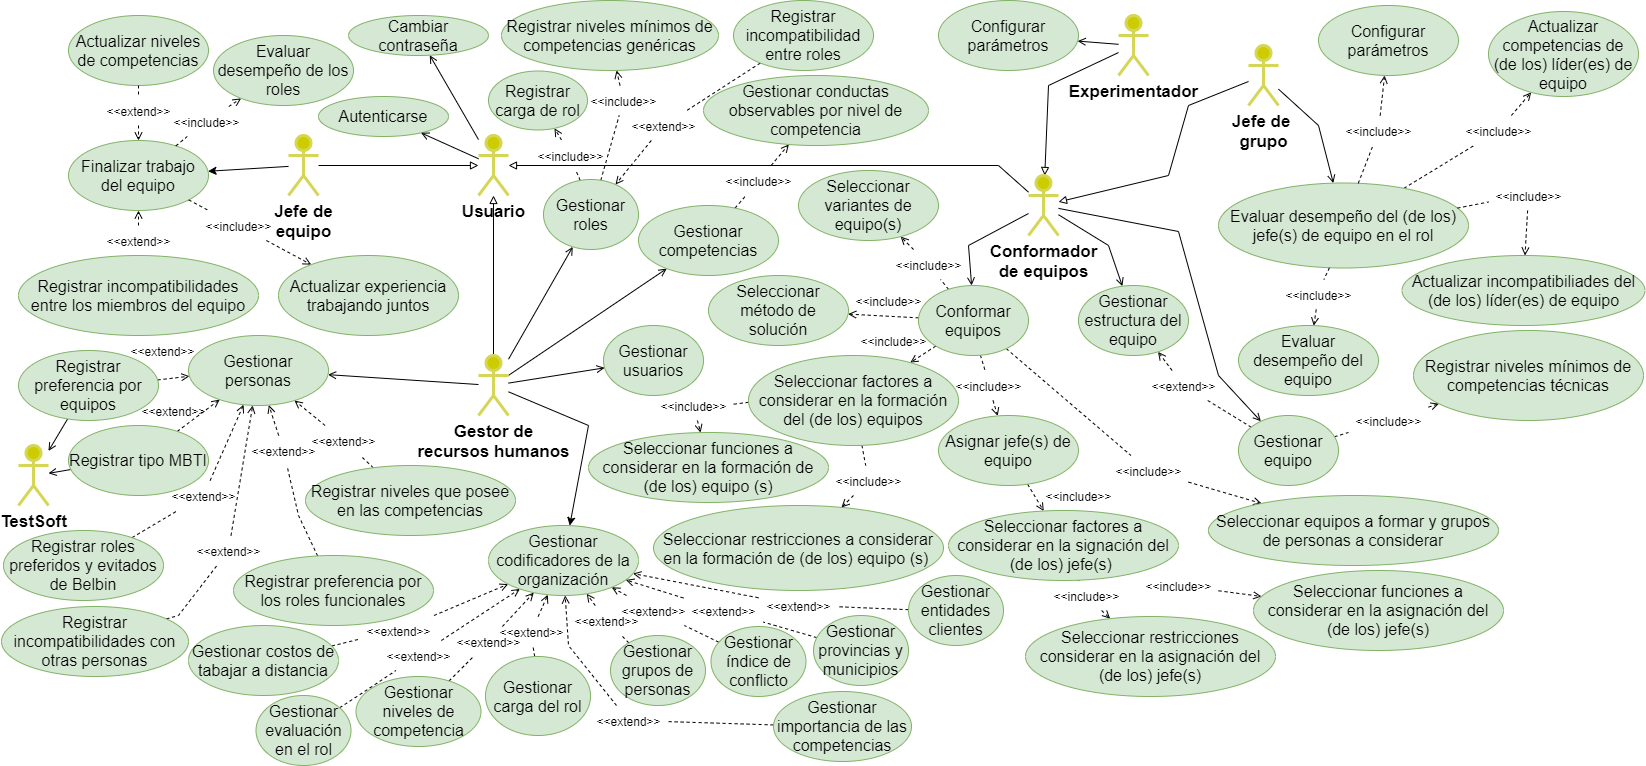
\includegraphics[width=1.2\textwidth]{figuras/diagrama_CUTeamSoft.png} 
	\caption{Diagrama de Caso de Uso del Sistema de TEAMSOFT$^+$. Recreado a partir de \cite{Duran2019}}  \label{fig:cuteamsoft}
\end{figure}

En la Figura \ref{fig:opcines_teamsoft} se observan las opciones implementadas en la herramienta. En la etapa de \textbf{Configuración} se establece las escalas de valores en la que se miden el nivel de cumplimiento de las competencias y los roles. En la opción \textbf{Personal}, se gestionan las competencias, roles y personas. Por último, en \textbf{Proyectos}, se gestionan los proyectos y se conforma el equipo de proyecto.\\

\begin{figure}[H]
	\centering
	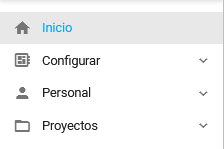
\includegraphics[width=0.5\textwidth]{figuras/opciones_team_soft.png} 
	\caption{Opciones de TEAMSOFT$^+$}\label{fig:opcines_teamsoft}
\end{figure}

El sistema realiza el proceso de asignación del personal en tres etapas. A continuación se explica en qué consiste cada una, y en la Figura \ref{fig:conf_equip_teamsoft} se observa el flujo entre ellas en TEAMSOFT$^+$:
\begin{description}
	\item[Primera etapa:] se configura la cantidad máxima de roles, se elijen los proyectos a conformar y además los grupos de personas que se van a tener en cuenta para el proceso de formación del equipo.
	\item[Segunda etapa:] se asigna el Jefe de Proyecto. En esta etapa se toman en cuenta los elementos definidos por el usuario para desempeñar este rol, por ejemplo: competencias técnicas y genéricas, tipos psicológicos, entre otros.
	\item[Tercera etapa:] se conforma el equipo. En la asignación del resto del equipo, se tienen en cuenta además, las incompatibilidades entre las personas y entre los roles del proyecto.
\end{description}

%El sistema realiza el proceso de asignación del personal en tres etapas (ver figura \ref{fig:conf_equip_teamsoft}), una primera de configuración, donde se establece la cantidad máxima de roles, se elijen los proyectos a conformar y además los grupos de personas que se van a tener en cuenta para el proceso de asignación. Las etapas restantes, como propone \cite{Institute2020}, asignan primero al Jefe de Proyecto (segunda etapa) y después, se conforma el equipo (tercera etapa). Al  asignar jefe del proyecto se tienen en cuenta los elementos definidos por el usuario para desempeñar este rol, por ejemplo: competencias técnicas y genéricas, tipos psicológicos, entre otros. En la asignación del resto del equipo, se tienen en cuenta además, las incompatibilidades entre las personas y roles en el proyecto.

\begin{figure}[H]
	\centering
	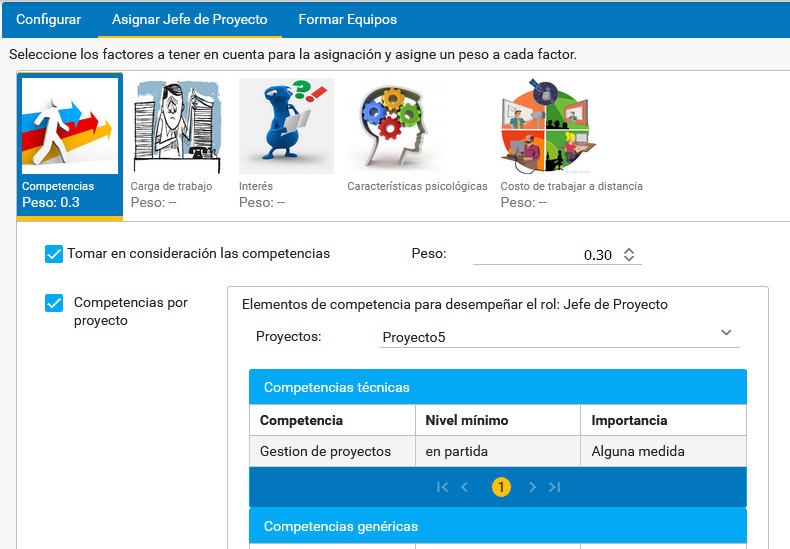
\includegraphics[width=1\textwidth]{figuras/conformacion_equipos_asignar_jefe.png}
	\caption{Flujo para conformar el equipo en TEAMSOFT$^+$}\label{fig:conf_equip_teamsoft}
\end{figure}


\section{Conformación de equipos de béisbol} \label{ej-pel}

El béisbol es un deporte con una amplia difusión en el continente americano y asiático, e incluso, en los últimos años se ha extendido al continente europeo. Se considera el deporte nacional en países como Cuba y Estados Unidos \cite{INEFI2020}. Dado el auge de este deporte, resulta de gran interés popular la conformación de un equipo de béisbol.\\

Un equipo de béisbol está compuesto por varios jugadores. Antes de cada juego, el director del equipo tiene que elegir 10 para la alineación inicial. Cada jugador, con excepción del pícher\footnote{anglicismo aceptado por la RAE para la voz inglés pitcher} y el bateador designado, tiene que desempeñar dos tipos de roles, uno a la defensiva y otro a la ofensiva. En el caso particular del pícher, solo está presente en la alineación defensiva, mientras que el bateador designado ocupa su puesto a la ofensiva. Resulta importante resaltar que un jugador no puede jugar más de un rol del mismo tipo en una alineación. Para cada tipo de rol, existen un conjunto de características o competencias a tener en cuenta para la asignación de un jugador. Por ejemplo, según \cite{Smith1995},  las competencias genéricas a tener en cuenta son:

\begin{itemize}
	\item Trabajo bajo presión (\textit{Peaking Under Pressure}): capacidad del jugador de sentirse desafiado en lugar de amenazado por la presión y su rendimiento bajo presión.
	
	\item Libre de preocupaciones (\textit{Freedom From Worry}): no se presiona a sí mismo, preocupándose por desempeñarse mal o cometer errores. No se ve afectado por las opiniones de los demás con respecto a su desempeño.
	
	\item Afrontar la adversidad (\textit{Coping With Adversity}): permanece positivo y entusiasta, incluso cuando las cosas van mal, permanece tranquilo y controlado; puede recuperarse rápidamente de errores y contratiempos.
	
	\item Concentración (\textit{Concentration}): No se distrae fácilmente; capaz de concentrarse en la tarea en cuestión en tanto en situaciones de práctica como de juego, incluso cuando ocurren situaciones adversas o inesperadas.
	
	\item Preparación mental (\textit{Mental Preparation}): planea y se prepara mentalmente para los juegos y claramente tiene un “plan de juego" para lanzar, batear, correr bases, etc.
	
	\item Motivación para el logro (\textit{Achievement Motivation}): tiene confianza y está motivado positivamente; constantemente da el 100\% durante las prácticas y los juegos; trabaja duro para mejorar sus habilidades.
	
	\item Entrenabilidad (\textit{Coachability}): abierto y aprende de la instrucción; acepta la crítica constructiva sin tomárselo personalmente y enojarse.
\end{itemize}

En el caso de las competencias técnicas a cumplir por un jugador, en una alineación, según \cite{2020a, Silverman2011} son:
\begin{itemize}
	\item Promedio de bateo.
	\item Fuerza de bateo.
	\item Precisión de tiro. 
	\item Fildeo.
	\item Velocidad.
	\item Versatilidad.
\end{itemize}

En la literatura existen diversas investigaciones relacionadas con la conformación de equipos de béisbol. En \cite{Polyashuk2015, Sugrue2007} los autores se basan en las estadísticas de los jugadores almacenadas a lo largo de los años para construir un indicador. En base a este indicador es que se realiza el proceso de asignación de los jugadores a los roles. Las investigaciones planteadas anteriormente, solo se enfocan en la conformación de la alineación ofensiva (orden al bate), sin tener en cuenta la alineación defensiva. Además, no tienen en cuenta las competencias que necesitan los roles para ser ocupados, y tampoco hacen referencia a la preferencia de las personas por los roles.

\section{Conformación de equipos docentes} \label{ej-carga}

La planificación de la carga docente es un problema recurrente en cada inicio de semestre para los encargados en cada centro de educación. En el proceso de asignación de la carga docente intervienen dos aspectos fundamentales: el claustro de profesores disponibles y el conjunto de asignaturas a impartir.\\

En \cite{res2018} se define cómo organizar el proceso docente de cada asignatura, siendo imprescindible conocer, la cantidad de horas asociadas a cada forma de enseñanza, estas son:
\begin{itemize}
	\item Conferencia(C)
	\item Clase práctica(CP)
	\item Seminario(S)
	\item Laboratorio(L)
	\item Taller(T)
\end{itemize}

Cada forma de enseñanza se puede considerar como los roles a desempeñar por los profesores en el colectivo de asignatura. Cada uno de estos roles tiene asociado un conjunto de competencias que debe satisfacer el profesor para desempeñarlo correctamente. Por ejemplo \cite{res2016} recomienda que las conferencias sean impartidas por un profesor de experiencia, entre otros aspectos.\\

Del claustro de profesores se conocen sus competencias, preferencias y disponibilidad. Por ejemplo: la categoría docente y científica, los años de experiencia impartiendo las asignaturas, el fondo de tiempo disponible para la docencia y, el interés por las asignaturas, entre otras. Las categorías docentes que puede alcanzar un profesor están definidas en \cite{res2016}, estas son:
\begin{itemize}
	\item Profesor Titular
	\item Profesor Auxiliar
	\item Profesor Asistente
	\item Instructor
\end{itemize} 

El jefe de departamento es el encargado de elaborar el Plan de resultado de cada profesor y, al finalizar el año verificar su cumplimento. En función del cumplimiento del plan, se le otorga a cada profesor una evaluación general. La evaluación general se otorga a partir de un consenso entre las siguientes seis dimensiones \citep{Ansola2020}:
\begin{itemize}
	\item \textbf{Docente}. Clases impartidas (cantidad de grupos y asignaturas, tipos de clase) así como la calidad de ellas. Las tutorías de tesis y prácticas profesionales.
	\item \textbf{Metodológico}. Cumplimiento del Plan Metodológico de la Asignatura (planificación de las clases y otras actividades), cumplimiento del Plan de Controles a Clases del Departamento.
	\item \textbf{Superación}. Cambio o ratificación de categoría docente, cursos de superación o postgrado.
	\item \textbf{Investigación}. Publicaciones en revistas, libros, premios.
	\item \textbf{Extensión universitaria}. Participación en: donaciones de sangre, juegos 13/3 para trabajadores, cuidado de Pruebas de Ingreso a la Educación Superior, entre otras actividades que se puedan realizar en la Universidad.
	\item \textbf{Política}. Actitud ante los estudiantes y resto de los compañeros, cumplimiento de la Guardia Obrera, participación en actividades políticas y de masa organizadas por la Universidad o el país. Pertenencia a organizaciones políticas (UJC-PCC).
\end{itemize}

Muchas universidades del mundo tienen que enfrentar el proceso de asignar profesores a los tipos de clases que le corresponden a las asignaturas, al menos una vez al año. En la literatura existen múltiples investigaciones que se enfocan en la asignación de los profesores a las asignaturas. Por ejemplo, en \cite{Domenech2014} se presenta un modelo donde se realiza el proceso de conformación del equipo asignando los profesores a las asignaturas. Este trabajo tiene en cuenta el balance de la carga de los profesores y sus preferencias hacia las asignaturas. En \cite{Bosquez2020} se propone otro modelo para la asignación de asignaturas a profesores, basándose en la preferencia de los mismos hacia las asignaturas (si le interesaba darla o no). En ninguno de los trabajos revisados los autores tienen en cuenta para realizar la asignación, las competencias de los profesores, ni las competencias necesarias para cada cumplir cada rol. Tampoco hacen referencia a las incompatibilidades que pueden existir entre los miembros del colectivo de una asignatura.

\section{Conclusiones parciales}
Una vez terminado el capítulo se arriban a las siguientes conclusiones:
\begin{enumerate}
	\item Existe un modelo definido para el problema de conformación de equipos de software que tiene propiedades generales, debido a que incluye personas, roles, competencias.
	\item Existe una herramienta que le da soporte al modelo de conformación de equipos de software denominada TEAMSOFT$^+$.
	\item Para los problemas de conformación de equipos docentes y de béisbol no existen modelos definidos que tengan en cuenta las competencias de las personas para ocupar los roles, las incompatibilidades entre las personas y las preferencias por los roles.
	\item Tanto el modelo como la herramienta TEAMSOFT$^+$ podrían se aplicados para formar equipos docentes y de béisbol, ya que toman en cuenta los factores a considerar en cada caso.
\end{enumerate}
\pagebreak
%\subsection{Requisitos funcionales}
%\begin{itemize}
%	 \item Realizar la modelación de los datos correspondientes a lo descrito en la sección \ref{chap:descripcion}, incluyendo un nombre para cada entidad descrita.
%	\item Desarrollar la base de datos que se corresponde con el modelo identificado.
%	\item Implementar la carga de datos a partir de un fichero de entrada, para otorgar valores a los conjuntos descritos en la sección \ref{entidades}.
%	\item Importar y exportar la base de datos.
%\end{itemize}
%\subsection{Requisitos no funcionales}
%\begin{itemize}
%	\item La interfaz deben mantener un mismo patrón de diseño que resulte comprensible al usuario. 
%	\item Utilizar un método para el control de versiones.
%\end{itemize}
%
%%\section{Conclusiones parciales}
%%Al terminar de leer el capítulo se puede concluir que:
%%\begin{itemize}
%%	\item Con el trabajo rela.
%%\end{itemize}
	\chapter[Factibilidad de aplicar TEAMSOFT$^+$ en equipos docentes y de béisbol]{Análisis de la factibilidad de aplicar la herramienta TEAMSOFT$^+$ y el modelo al cual le brinda soporte en la formación de equipos de docencia y de béisbol}\label{chap:2}

En el presente capítulo se describe cómo pueden definirse los problema de formación de equipos de béisbol y docentes empleando como base el modelo para la formación de equipos de proyectos de software soportado por la herramienta \hyperref[sec:modelo-teamsoft]{TEAMSOFT$^+.$} Esto implica que para cada problema se utilizarán o no, algunas de las relaciones propuestas en este modelo. También se describe una propuesta para obtener los valores de las competencias de las personas a partir de información que hoy se gestiona sobre ellas.

\section{Ejemplo simple para el problema de formación de equipos de béisbol}\label{ejemplo-pel}

Partiendo del modelo de formación de equipos de software, descrito en la Sección \ref{sec:modelo-teamsoft}, se ejemplificará con una instancia, una aproximación del problema de formación de equipos de béisbol. Se recomienda el análisis futuro de otros roles como el emergente o los roles asociados al picheo como abridores o relevistas que tienen otra complejidad.

\subsection{Conjuntos que intervienen en la modelación}\label{sec:conjuntos}
{\color{red}
Un equipo está compuesto por una nómina de jugadores, generalmente más de 20, entre los cuales se escoge la alineación regular. Esta alineación se compone de 9  jugadores (excluyendo al pícher) que tienen que jugar 18 roles. Además, los mismos jugadores asignados a roles defensivos tienen que estar asignados a roles ofensivos. Estos roles están divididos en dos categorías o tipos (ver Tabla \ref{tipo-roles}).
}
\begin{table}[H]
	\centering
	\caption{Tipos de roles}\label{tipo-roles}
	\scalebox{0.95}{
	\begin{tabular}{l	 c}
		\toprule[1.7pt]
		\textbf{Roles defensivos} & \textbf{Roles ofensivos} \\ \midrule
		      receptor (C)        & 1$^{er}$ bate (B1)       \\
		      1ra base (1B)       & 2$^{do}$ bate (B2)       \\
		      2da base (2B)       & 3$^{er}$ bate (B3)       \\
		    campo corto (SS)      & 4$^{to}$ bate (B4)       \\
		      3ra base (3B)       & 5$^{to}$ bate (B5)       \\
		jardinero izquierdo (LF)  & 6$^{to}$ bate (B6)       \\
		 jardinero central (CF)   & 7$^{mo}$ bate (B7)       \\
		 jardinero derecho (RF)   & 8$^{vo}$ bate (B9)       \\
		 bateador designado (BD)  & 9$^{no}$ bate (B9)       \\ \bottomrule[1pt]
	\end{tabular}
}
\end{table}

\begin{itemize}	
	\item $P=\{p_1, p_2\ldots\}$: Conjunto de jugadores, $p = 1...|25|$.
	
	\item $T=\{t_1=batear\;con\;hombres\;en\;base, t_2=fuerza\;de\;bateo, t_3=precisi\acute{o}n\;de\;tiro, t_4=velocidad, t_5=versatilidad, t_6=capacidad\;de\;embase\}$: Conjunto de competencias técnicas, $t= 1\ldots|T|$, $|T|=6$. \label{compt-pel}
	
	\item $G=\{g_1=trabajo\;bajo\;presi\acute{o}n
	, g_2=libre\;de\;preocupaciones, g_3=concentraci\acute{o}n,$ $g_4=afrontar\;la\;adversidad, g_5=preparaci\acute{o}n\;mental, g_6=entrenabilidad,$ $g_7=motivaci\acute{o}n\;para\;el\;logro\}$: Conjunto de competencias genéricas, $g= 1\ldots |G|$, $|G|=7$.
	
	\item $R=\{r_1=C,r_2=1B,r_3=2B,r_4=SS,r_5=3B,r_6=LF,r_7=CF,r_8=RF,r_{9}=BD,r_{10}=B1,r_{11}=B2,r_{12}=B3,r_{13}=B4,r_{14}=B5,r_{15}=B6, r_{16}=B7,r_{17}=B8,r_{18}=B9\}$: Conjunto de roles, $r = 1\ldots |R|$, $|R|=18$. \label{def-roles-pel} 
	
	\item $Y={y_1}$: Un solo equipo a formar.
	
\end{itemize}


Las relaciones se van a dividir en dos secciones. La primera sección trata los aspectos genéricos del problema, que no cambian en función de los integrantes, o del equipo. La segunda sección va a un nivel más específico, que está en dependencia de las personas a asignar. Los valores asignados en la Sección \ref{asp-gen-pel} son todos a consideración del autor, y además configurables.

\subsection{Elementos generales} \label{asp-gen-pel}

En las Tablas \ref{mcgd-pel} y \ref{mcgo-pel} se muestran los valores mínimos necesarios que las personas deben tener en las competencias genéricas para desempeñar cada rol a la defensiva y a la ofensiva, respectivamente. Por ejemplo, para poder jugar el rol $C$ es necesario que la persona tenga como mínimo un valor en la competencia genérica $g_1$ de 0.8. 

 
\begin{table}[H]
	\caption{Valores mínimos de las competencias genéricas para cada rol defensivo}\label{mcgd-pel}
	\centering
	\begin{tabular}{|l|c|c|c|c|c|c|c|c|c|}
		\hline
		$Z(g,r)$ & $C$ & $1B$  & $2B$ & $SS$ & $3B$ & $LF$ & $CF$ & $RF$ & $BD$ \\ \hline
		$g_1=trabajo\;bajo\;presi\acute{o}n$ & 0.8 & 0.6 & 0.6 & 0.6 & 0.6 & 0.5 & 0.5 & 0.5 & 0.3
		\\ \hline
		$g_2=libre\;de\;preocupaciones$ & 0.7 & 0.6 & 0.7 & 0.7 & 0.6 & 0.7 & 0.7 & 0.7 & 0.3\\ \hline
		$g_3=concentraci\acute{o}n$ & 0.8 & 0.7 & 0.7 & 0.7 & 0.7 & 0.6 & 0.6 & 0.6 & 0.5 \\ \hline
		$g_4=afrontar\;la\;adversidad$ & 0.6 & 0.5 & 0.5 & 0.5 & 0.5 & 0.5 & 0.4 & 0.4 & 0.3 \\ \hline
		$g_5=preparaci\acute{o}n\;mental$ & 0.7 & 0.3 & 0.3 & 0.3 & 0.3 & 0.3 & 0.3 & 0.3 & 0.3 \\ \hline
		$g_6=entrenabilidad$ & 0.5 & 0.5 & 0.5 & 0.5 & 0.5 & 0.5 & 0.5 & 0.5 & 0.4\\ \hline
		$g_7=motivaci\acute{o}n\;para\;el\;logro$ & 0.5 & 0.5 & 0.5 & 0.5 & 0.5 & 0.5 & 0.5 & 0.5 & 0.4\\ \hline
	\end{tabular}
\end{table}

\begin{table}[H]
	\caption{Valores mínimos de las competencias genéricas para cada rol ofensivo}\label{mcgo-pel}
	\centering
	\begin{tabular}{|l|c|c|c|c|c|c|c|c|c|}
		\hline
		\thead{$Z(g,r)$} & $B1$ & $B2$  & $B3$ & $B4$ & $B5$ & $B6$ & $B7$ & $B8$ & $B9$ \\ \hline
		$g_1=trabajo\;bajo\;presi\acute{o}n$ 	 & 0.6 	&  0.6 	&  0.7 &  0.7 &  0.7 &  0.5 &  0.5 & 0.5  & 0.4 \\ \hline
		$g_2=libre\;de\;preocupaciones$ 	 & 0.5  &  0.5  &  0.5 &  0.5 &  0.4 &  0.4 &  0.4 & 0.4  & 0.3 \\ \hline
		$g_3=concentraci\acute{o}n$ 	 & 0.7  &  0.7  &  0.7 &  0.7 &  0.7 &  0.6 &  0.6 & 0.6  & 0.5 \\ \hline
		$g_4=afrontar\;la\;adversidad$ 	 & 0.6  &  0.5  &  0.5 &  0.5 &  0.5 &  0.5 &  0.4 & 0.4  & 0.3 \\ \hline
		$g_5=preparaci\acute{o}n\;mental$ 	 & 0.7  &  0.6  &  0.6 &  0.7 &  0.7 &  0.6 &  0.5 & 0.5  & 0.4 \\ \hline
		$g_6=entrenabilidad$ 	 & 0.5  &  0.5  &  0.5 &  0.5 &  0.5 &  0.5 &  0.5 & 0.5  & 0.5 \\ \hline
		$g_7=motivaci\acute{o}n\;para\;el\;logro$ 	 & 0.6  &  0.6  &  0.6 &  0.6 &  0.6 &  0.6 &  0.6 & 0.6  & 0.6 \\ \hline
	\end{tabular}
\end{table}


%--------inicio-y1-------------
 
En las Tablas \ref{mctd1-pel} y \ref{mcto1-pel} se muestran los valores mínimos necesarios que las personas deben tener en las competencias técnicas para desempeñar cada rol. Las posiciones defensivas no requieren de competencias relacionadas con la ofensiva ($t_1=$ \textit{batear con hombres en base}, $t_2=$ \textit{fuerza de bateo}, $t_6=$ \textit{capacidad de embase}), por lo tanto, a cada rol defensivo se le otorga el valor de 0.0 en las competencias relacionadas con la ofensiva. El bateador designado es un caso excepcional, aunque clasificado como un rol defensivo, no tiene competencias defensivas que lo definan como tal. Esto significa que, aunque realmente no juega a la defensiva, es necesario tenerlo en cuenta para ocupar un rol a la ofensiva. Por lo tanto, se asocian a este rol, las competencias que tienen tendencia ofensiva.
\begin{table}[H]
	\centering
	\caption{Valores mínimos de las competencias técnicas para cada rol defensivo en el equipo $y_1$}\label{mctd1-pel}
	\begin{tabular}{|l|c|c|c|c|c|c|c|c|c|}
		\hline
		\thead{$Q(t,r,y)$} & $C$ & $1B$  & $2B$ & $SS$ & $3B$ & $LF$ & $CF$ & $RF$ & $BD$  \\ \hline
		$t_3=precisi\acute{o}n\;de\;tiro$ 		 & 0.8 &  0.5  &  0.6 & 0.6  & 0.7  & 0.7  & 0.7  &  0.7 & 0.0 \\ \hline
		$t_4=velocidad$ 		 & 0.2 &  0.2  &  0.2 & 0.2  & 0.2  & 0.7  & 0.8  &  0.7 &  0.4 \\ \hline
		$t_5=versatilidad$   	 & 0.2 &  0.3  &  0.5 & 0.5  & 0.5  & 0.6  & 0.6  &  0.6 & 0.0 \\ \hline
	\end{tabular}
\end{table}

Los roles ofensivos no necesitan tener habilidades defensivas, como es el caso de la competencia técnica $t_3=precisi\acute{o}n\;de\;tiro$. Por este motivo no se muestra en la Tabla \ref{mcto1-pel}.

\begin{table}[H]
	\centering
	\caption{Valores mínimos de las competencias técnicas para cada rol ofensivo en el equipo $y_1$}\label{mcto1-pel}
	\begin{tabular}{|l|c|c|c|c|c|c|c|c|c|}
		\hline
		\thead{$Q(t,r,y)$} & $B1$ & $B2$ & $B3$ & $B4$ & $B5$ & $B6$ & $B7$ & $B8$ & $B9$  \\ \hline
		$t_1=batear\;con\;hombres\;en\;base$ 	     & 0.6  & 0.7  & 0.8  & 0.8  & 0.7  & 0.7  & 0.5  & 0.5  & 0.5 \\ \hline
		$t_2=fuerza\;de\;bateo$ 		 & 0.5  & 0.6  & 0.7  & 0.8  & 0.7  & 0.6  & 0.5  & 0.4  & 0.4 \\ \hline
		$t_4=velocidad$ 		 & 0.7  & 0.5  & 0.4  & 0.3  & 0.3  & 0.3  & 0.3  & 0.2  & 0.1 \\ \hline
		$t_5=versatilidad$   	 & 0.3  & 0.3  & 0.3  & 0.3  & 0.2  & 0.3  & 0.3  & 0.1  & 0.3 \\ \hline
		$t_6=capacidad\;de\;embase$ & 0.8 &  0.7  &  0.6 & 0.6  & 0.6  & 0.5  & 0.5  &  0.4 & 0.4 \\ \hline
	\end{tabular} 
\end{table}
%----------------fin--y1-----------------


%---------------inicio----------------------

%----------------nuevo----------------

Anteriormente se explicó que en un equipo de béisbol, cada jugador ocupa dos roles (excepto el pícher y el bateador designado), uno a la defensiva y otro a la ofensiva. La Tabla \ref{cmrpp-pel} muestra lo planteado.
\begin{table}[H]
	\centering
	\caption{Cantidad máxima de roles por persona a jugar en un equipo de béisbol }\label{cmrpp-pel}
	\begin{tabular}{|c|c|c|c|c|c|c|c|c|c|}
		\hline
		$K_{py}(p,y)$ & $p_1$ & $p_2$ & $p_3$  & $p_4$ & $p_5$ & $p_6$ & $p_7$  & $p_8$ & $p_9$ \\ \hline
		$y_1$ & 2 & 2 & 2 & 2 & 2 & 2 & 2 & 2 & 2 \\ \hline
	\end{tabular}
\end{table}

%-----------------------------------

Las incompatibilidades entre los roles como ya se mencionaba, está dada por el tipo de rol. Todos los roles ofensivos (por ejemplo, B1, B2, B3) tienen incompatibilidades entre ellos, y son compatibles con los defensivos (por ejemplo, C, 3B, CF). Sucede lo mismo con los roles defensivos: son incompatibles entre ellos y compatibles con los ofensivos. Debido a la número tan alto de incompatibilidades (144\footnote{Son 18 roles, 9 por cada tipo, cada uno es incompatible con los 8 del mismo, por tanto $8*18=144$}), en la Tabla \ref{ier1-pel} solo se pone un subconjunto de los roles.
\begin{table}[H]
	\centering
	\caption{Incompatibilidades entre roles}\label{ier1-pel}
	\begin{tabular}{|c|c|c|c|c|c|c|}
		\hline
		$I_r(r,u,y)$  & $B1$& $B2$& $B3$& $C$ & $3B$& $CF$  \\ \hline
		$B1$ 			&  0  &  1  &  1  &  0  &  0  &  0 \\ \hline
		$B2$ 			&  1  &  0  &  1  &  0  &  0  &  0 \\ \hline
		$B3$ 			&  1  &  1  &  0  &  0  &  0  &  0 \\ \hline
		$C$		    	&  0  &  0  &  0  &  0  &  1  &  1 \\ \hline
		$3B$			&  0  &  0  &  0  &  1  &  0  &  1 \\ \hline
		$CF$ 			&  0  &  0  &  0  &  1  &  1  &  0 \\ \hline
	\end{tabular}
 \end{table}


La cantidad de personas necesarias para jugar un rol en una alineación siempre será una sola, sin importar el tipo de rol, y el equipo.\\

\subsection{Elementos específicos} \label{asp-espec-pel}

Después de ver los aspectos generales del modelo, es necesario instanciar tanto las personas como el equipo en cuestión, para lograr un ejemplo completo. Todos los valores otorgados en esta sección son ficticios. Más adelante, en la Sección \ref{sec:tran_pel} se hace una propuesta para la obtención de estos datos a partir de fuentes externas.

\begin{itemize}
	\item $P=\{p_1=frank, p_2=rudy, p_3=carlos, p_4=alexander, p_5=juan, p_6=yurisbel, p_7=jos\acute{e},p_8=pedro,p_9=pepe, p_{10}=camilo, p_{11}=oscar, p_{12}=roberto, p_{13}=enrique, p_{14}=yasel, p_{15}=dayron\}$: Conjunto de personas, $p = 1...|P|$, $|P|=15$.
	
	\item $Y=Industriales$: Equipo a formar.
\end{itemize}

En la Tabla \ref{iep-pel} se muestra un posible ejemplo de las incompatibilidades entre los jugadores del equipo Industriales (generado de forma aleatoria sin ninguna base real). Es importante destacar que la relación de incompatibilidad no tiene que ser la misma en ambos sentidos, por ejemplo $p_1$  es totalmente incompatible con $p_2$, mientras que $p_2$ es compatible con $p_1$.
		
\begin{table}[H]
	\centering
	\caption{Incompatibilidades entre personas del equipo $Industriales$}\label{iep-pel}
	\begin{tabular}{|c|c|c|c|c|c|c|c|c|c|}
		\hline
		$I_p(p,q)$ & $p_1$ & $p_2$ & $p_3$  & $p_4$ & $p_5$ & $p_6$ & $p_7$ & $p_8$  & $p_9$ \\ \hline
		$p_1$ 	& 0.0 & 1.0 & 0.3 & 0.2 & 0.4 & 0.0 & 0.4 & 0.3 & 0.2 \\ \hline
		$p_2$  	& 0.3 & 0.0 & 0.9 & 0.0 & 0.1 & 0.8 & 0.0 & 0.9 & 0.0 \\ \hline
		$p_3$ 	& 0.5 & 0.2 & 0.0 & 0.3 & 0.2 & 0.5 & 0.2 & 0.0 & 0.3 \\ \hline
		$p_4$ 	& 0.6 & 0.3 & 0.5 & 0.0 & 0.3 & 0.3 & 0.5 & 0.0 & 0.3 \\ \hline
		$p_5$ 	& 0.1 & 0.7 & 0.1 & 0.8 & 0.0 & 0.1 & 0.7 & 0.1 & 0.8 \\ \hline
		$p_6$ 	& 0.0 & 1.0 & 0.3 & 0.2 & 0.4 & 0.0 & 0.9 & 0.3 & 0.2 \\ \hline
		$p_7$  	& 1.0 & 0.0 & 0.9 & 0.0 & 0.1 & 1.0 & 0.0 & 0.9 & 0.0 \\ \hline
		$p_8$ 	& 0.5 & 0.2 & 0.0 & 0.3 & 0.2 & 0.5 & 0.2 & 0.0 & 0.3 \\ \hline
		$p_9$ 	& 0.6 & 0.3 & 0.5 & 0.0 & 0.3 & 0.3 & 0.5 & 0.0 & 0.0 \\ \hline
	\end{tabular}
\end{table}


%---------------------inicio--------------

Las personas tienen un valor de preferencia por desempeñar cada rol. Por ejemplo, en la Tabla \ref{prd-pel} se puede decir que la persona $ p_3 $ tiene poca preferencia por el rol $ 3B $, mientras que en la Tabla \ref{pro-pel} un valor de preferencia alto por el rol $B1$.
\begin{table}[H]
	\centering
	\caption{Preferencias de las personas por los roles defensivos}\label{prd-pel}
	\begin{tabular}{|c|c|c|c|c|c|c|c|c|c|}
		\hline
		$F_r(p,r)$ & $C$ & $1B$ & $2B$ & $SS$ & $3B$ & $LF$ & $CF$ & $RF$  & $BD$   \\ \hline
		$p_1$   & 0.6 & 0.2 & 0.5 & 0.6 & 0.8 & 0.6 & 0.2 & 0.5 & 0.6 \\ \hline
		$p_2$   & 0.2 & 0.3 & 0.6 & 0.4 & 0.5 & 0.2 & 0.3 & 0.6 & 0.4 \\ \hline
		$p_3$  	& 0.9 & 0.2 & 0.3 & 0.2 & 0.1 & 0.9 & 0.2 & 0.3 & 0.2 \\ \hline
		$p_4$ 	& 0.7 & 0.1 & 0.1 & 0.3 & 0.2 & 0.7 & 0.1 & 0.1 & 0.3 \\ \hline
		$p_5$   & 0.1 & 1.0 & 0.2 & 0.1 & 0.6 & 0.8 & 1.0 & 0.5 & 0.1 \\ \hline
		$p_6$   & 0.6 & 0.2 & 0.5 & 0.6 & 0.7 & 0.6 & 0.2 & 0.5 & 0.6 \\ \hline
		$p_7$   & 0.2 & 0.3 & 0.6 & 0.4 & 0.5 & 0.2 & 0.3 & 0.6 & 0.4 \\ \hline
		$p_8$  	& 0.9 & 0.2 & 0.3 & 0.2 & 0.1 & 0.9 & 0.2 & 0.3 & 0.2 \\ \hline
		$p_9$ 	& 0.7 & 0.1 & 0.1 & 0.3 & 0.2 & 0.7 & 0.1 & 0.1 & 0.3 \\ \hline
	\end{tabular}
\end{table}

\begin{table}[H]
	\centering
	\caption{Preferencias de las personas por los roles ofensivos}\label{pro-pel}
	\scalebox{.9}{
	\begin{tabular}{|c|c|c|c|c|c|c|c|c|c|}
		\hline
		$F_r(p,r)$ & $B1$& $B2$ & $B3$ & $B4$ & $B5$ & $B6$ & $B7$ & $B8$  & $B9$   \\ \hline
		$p_1$   & 0.7 & 0.3 & 0.6 & 0.4 & 0.5 & 0.6 & 0.1 & 0.7 & 0.5 \\ \hline
		$p_2$   & 0.2 & 0.5 & 0.4 & 0.7 & 0.7 & 0.5 & 0.5 & 0.3 & 0.7 \\ \hline
		$p_3$  	& 0.9 & 0.2 & 0.3 & 0.2 & 0.1 & 0.9 & 0.2 & 0.3 & 0.4 \\ \hline
		$p_4$ 	& 0.7 & 0.1 & 0.1 & 0.3 & 0.2 & 0.7 & 0.1 & 0.1 & 0.3 \\ \hline
		$p_5$   & 0.1 & 1.0 & 0.2 & 0.1 & 0.6 & 0.8 & 1.0 & 0.5 & 0.1 \\ \hline
		$p_6$   & 0.6 & 0.2 & 0.5 & 0.6 & 0.7 & 0.6 & 0.2 & 0.5 & 0.3 \\ \hline
		$p_7$   & 0.9 & 0.3 & 0.6 & 0.4 & 0.5 & 0.2 & 0.3 & 0.6 & 0.4 \\ \hline
		$p_8$  	& 0.5 & 0.6 & 0.4 & 0.7 & 0.5 & 0.3 & 0.7 & 0.8 & 0.3 \\ \hline
		$p_9$ 	& 0.7 & 0.4 & 0.9 & 0.2 & 0.2 & 0.5 & 0.3 & 0.5 & 0.0 \\ \hline
	\end{tabular}
}
\end{table}

%-----------------------fin-------------------------

En las Tablas \ref{pcg-pel} y \ref{pct-pel} se muestra el nivel que poseen las personas en las competencias genéricas y técnicas. Por ejemplo en la Tabla \ref{pcg-pel}, la persona $ p_1 $ tiene un valor alto en la competencia $ g_1 $.

\begin{table}[H]
	\centering
	\caption{Nivel de las personas en las competencias genéricas}\label{pcg-pel}
	\begin{tabular}{|l|c|c|c|c|c|c|c|c|c|}
		\hline
		\thead{$F_g(g,p)$} & $p_1$ & $p_2$ & $p_3$ & $p_4$ & $p_5$ & $p_6$ & $p_7$ & $p_8$ & $p_9$ \\ \hline  
		$g_1=trabajo\;bajo\;presi\acute{o}n$ 	& 0.7 & 0.5 & 0.3 & 0.6 & 0.8 & 0.4 & 0.3 & 0.7 & 0.1 \\ \hline
		$g_2=libre\;de\;preocupaciones$  	& 0.6 & 0.4 & 0.2 & 0.7 & 0.3 & 0.6 & 0.5 & 0.2 & 0.6 \\ \hline
		$g_3=concentraci\acute{o}n$ 	& 0.7 & 0.5 & 0.3 & 0.6 & 0.8 & 0.4 & 0.3 & 0.7 & 0.1 \\ \hline
		$g_4=afrontar\;la\;adversidad$  	& 0.6 & 0.4 & 0.2 & 0.7 & 0.3 & 0.6 & 0.9 & 0.2 & 0.6 \\ \hline
		$g_5=preparaci\acute{o}n\;mental$ 	& 0.7 & 0.5 & 0.3 & 0.6 & 0.8 & 0.9 & 0.3 & 0.7 & 0.1 \\ \hline
		$g_6=entrenabilidad$ 	& 0.5 & 0.6 & 0.4 & 0.3 & 0.5 & 0.7 & 0.5 & 0.6 & 0.2 \\ \hline
		$g_7=motivaci\acute{o}n\;para\;el\;logro$  	& 0.8 & 0.7 & 0.3 & 0.5 & 0.8 & 0.5 & 0.8 & 0.6 & 0.2 \\ \hline
		
	\end{tabular}
\end{table}

\begin{table}[H]
	\centering
	\caption{Nivel de las personas en las competencias técnicas}\label{pct-pel}
	\begin{tabular}{|l|c|c|c|c|c|c|c|c|c|}
		\hline
		\thead{$F_g(t,p)$}                   & $p_1$ & $p_2$ & $p_3$ & $p_4$ & $p_5$ & $p_6$ & $p_7$ & $p_8$ & $p_9$ \\ \hline
		$t_1=batear\;con\;hombres\;en\;base$ &  0.6  &  0.7  &  0.8  &  0.7  &  0.5  &  0.9  &  0.6  &  0.7  &  0.8  \\ \hline
		$t_2=fuerza\;de\;bateo$              &  0.7  &  0.8  &  0.6  &  0.7  &  0.1  &  0.5  &  0.2  &  0.3  &  0.3  \\ \hline
		$t_3=precisi\acute{o}n\;de\;tiro$    &  0.5  &  0.3  &  0.4  &  0.2  &  0.6  &  0.7  &  0.3  &  0.8  &  0.8  \\ \hline
		$t_4=velocidad$                      &  0.4  &  0.5  &  0.3  &  0.3  &  0.5  &  0.6  &  0.2  &  0.7  &  0.7  \\ \hline
		$t_5=versatilidad$                   &  0.5  &  0.7  &  0.6  &  0.7  &  0.6  &  0.3  &  0.8  &  0.6  &  0.1  \\ \hline
		$t_6=capacidad\;de\;embase$          &  0.7  &  0.4  &  0.7  &  0.5  &  0.8  &  0.9  &  0.5  &  0.5  &  0.6  \\ \hline
	\end{tabular}
\end{table}

La carga de trabajo empleada en el modelo de TEAMSOFT$^+$ no se utiliza, debido a que los jugadores de béisbol no pueden estar en varios equipos de béisbol al mismo tiempo.

%\begin{minipage}{12cm}
%\begin{landscape}

\subsection{Transformación de los datos}\label{sec:tran_pel}
{\color{red}
Para llevar a la práctica el modelo descrito en la Sección \ref{ejemplo-pel}, es necesario instanciar los conjuntos y relaciones con datos reales del problema. En el béisbol como en otros deportes existen indicadores para medir el desempeño de los jugadores. En Cuba, el \href{www.beisbolcubano.cu}{sitio web} de la Serie Nacional registra los indicadores más utilizados en este deporte para cuantificar el desempeño de los jugadores cubanos. Los datos utilizados en este trabajo fueron descargados de este sitio. Los indicadores son utilizados para determinar el nivel de un jugador en las competencias técnicas definidas por cada posición en este deporte. A continuación se describe brevemente cada indicador agrupado en dos categorías: bateo y fildeo.\\
}

\large{\textbf{Bateo}:}
\normalsize
\begin{itemize}
		\setlength\itemsep{0em}
	\item \textbf{CB}: comparecencias al bate. Todas las veces que el bateador se dispone a batear.
	\item \textbf{VB}: veces al bate ($ CB - (SF + SH + DB + BB)$).
	\item \textbf{C}: carreras anotadas por el jugador.
	\item \textbf{H}: \textit{Hits} conectados por el jugador.
	\item \textbf{AVE}: promedio de bateo ($ H/VB $).
	\item \textbf{OBP}: porcentaje de embasado ($(H + BB + DB) / (VB + BB + DB + SF)$).
	\item \textbf{2B}: dobles. \textit{Hits} que llevan al bateador a segunda base.
	\item \textbf{3B}: triples. \textit{Hits} que llevan al bateador a tercera base.
	\item \textbf{HR}: \textit{home runs}. Pelotas que el bateador las saca del terreno de juego en territorio válido.
	\item \textbf{TB}: total de bases alcanzadas ($H+2B+(3B*2)+(HR*3)$).
	\item \textbf{SLU}: porcentaje de \textit{slugging} ($ TB / H $).
	\item \textbf{OPS}: porcentaje de embasado más \textit{slugging} ($ OBP + SLU $).
	\item \textbf{BR}: bases robadas con éxito.
	\item \textbf{CR}: bases robadas fallidas.
	\item \textbf{CI}: carreras impulsadas.
	\item \textbf{SH}: \textit{hit} de sacrificio. Cuando un bateador, con el objetivo de que avancen los jugadores de base, hace contacto con la pelota y sale un \textit{rolling}. El jugador puede: no embasarse porque fue puesto \textit{out}, embasarse por error de la defensa o porque el jugador a la defensa decide tirar a otra base.
	\item \textbf{SF}: \textit{fly} de sacrificio. Cuando un bateador, con el objetivo de que avancen los jugadores de base, hace contacto con la pelota y sale un \textit{fly}.
	\item \textbf{DB}: pelotazo. Cuando un pícher golpea a un bateador.
	\item \textbf{BB}: bases por bolas. Cuando un bateador se embasa en primera, debido a que recibió cuatro bolas en su turno al bate.
	\item \textbf{SO}: ponche. Cuando un bateador recibe tres \textit{strikes}.
	\item \textbf{BD}: bateo para doble \textit{play}. Veces que debido al contacto que un bateador hizo con la pelota, el equipo contrario sacó dos \textit{outs}.
	\item \textbf{CPA}: cantidad de jugadores en posición anotadora cuando batea el jugador.
	\item \textbf{CIPA}: cantidad de veces que impulsa corredores en posiciones anotadoras (2$^{da}$ base y 3$^{ra}$ base).
	\item \textbf{JJ}: juegos jugados.
	\item \textbf{INN}: entradas jugadas.
\end{itemize}
\large{\textbf{Fildeo}:}
\normalsize
\begin{itemize}
		\setlength\itemsep{0em}
	\item \textbf{E}: errores cometidos.
	\item \textbf{TL}: total de lances. Cuando un jugador a la defensa lanza la pelota de una base a otra. 
	\item \textbf{AVE}: promedio de lances ($E/TL$).
	\item \textbf{DP}: doble $ plays $ realizados.
	\item \textbf{PB}: error que comete el receptor al controlar la pelota lanzada legalmente por el pitcher.
	\item \textbf{BR}: intentos de robo de base al receptor
	\item \textbf{CR}: robos de bases impedidos por el receptor.
	\item \textbf{POS}: posiciones jugadas por el pelotero.
\end{itemize}

En la Figura \ref{info-pelota} se muestran los datos de estos indicadores descargados del sitio web para los peloteros del equipo de Industriales.

%\newgeometry{left=1.5cm,right=1.5cm,top=2cm,bottom=.5cm} 

\newpage
\KOMAoptions{paper=landscape, pagesize}
\recalctypearea
\null\vfill
\pagestyle{plain}

\begin{figure} [H]
	\hspace{-2.6cm}  
%		\centering
	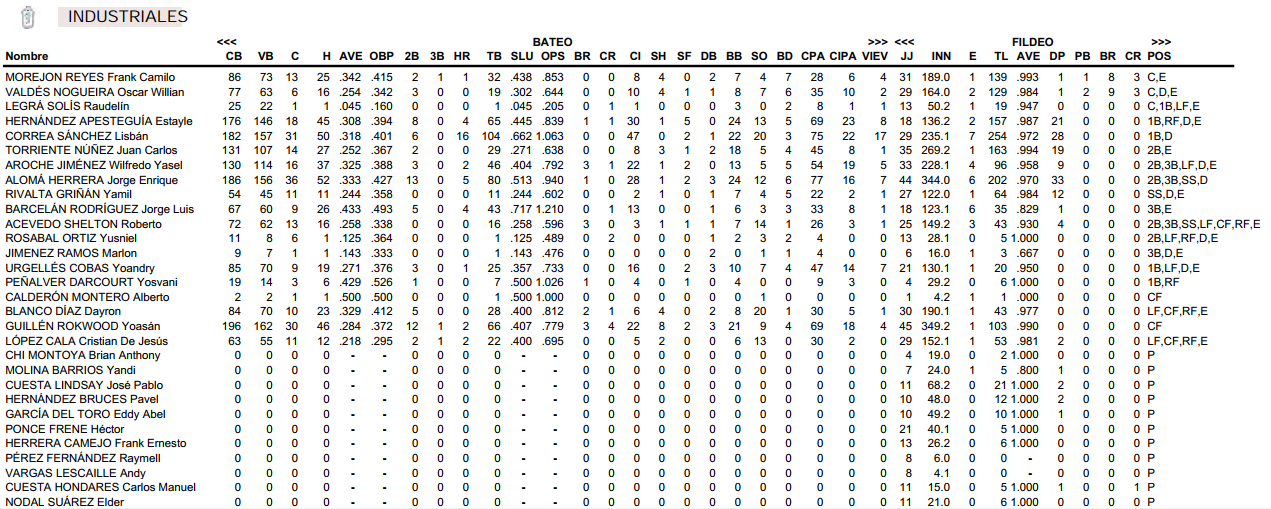
\includegraphics[width=1.25\textwidth]{figuras/informacionPelota.png}
	\caption[Información almacenada de los peloteros en el sitio web beisbolcubano.]{Información almacenada de los peloteros en el sitio web beisbolcubano \cite{INDER2020}}\label{info-pelota}
\end{figure}
\vfill\null
\newpage
\KOMAoptions{paper=portrait, pagesize}
\recalctypearea
\pagestyle{fancy} 


En la Tabla \ref{correspondencia-pel} se presenta la correspondencia entre los indicadores y las competencias técnicas definidas en la Sección \ref{compt-pel}. Además de estos indicadores, también existen otros que se pudiesen tener en cuenta, por ejemplo en la \textit{Major Ligue Baseball} (MLB) se maneja la velocidad de \textit{sprint} (SV) expresada en pies/segundos.

\begin{table} [H]
	\centering
	\caption{Correspondencia entre indicadores y competencias técnicas} \label{correspondencia-pel}
	\begin{tabular}{|l|c|}
		\hline
		\textbf{Competencias Técnicas}                                          & \textbf{Indicadores} \\ \hline
		\multirow{4}{6.3cm}{$\boldsymbol{t_1}=batear\;con\;hombres\;en\;base $} &          CI          \\
		                                                                        &          SH          \\
		                                                                        &          SF          \\
		                                                                        &       CIPA/CPA       \\ \hline
		\multirow{4}{6.3cm}{$\boldsymbol{t_2}=fuerza\;de\;bateo $}              &          2B          \\
		                                                                        &          3B          \\
		                                                                        &          HR          \\
		                                                                        &         SLU          \\ \hline
		$\boldsymbol{t_3}= precisi\acute{o}n\;de\;tiro $                        &     AVG (fildeo)     \\ \hline
		\multirow{4}{6.3cm}{$\boldsymbol{t_4}= velocidad $}                     &          BR          \\
		                                                                        &          CR          \\
		                                                                        &          2B          \\
		                                                                        &          3B          \\ \hline
		$\boldsymbol{t_5}= versatilidad $                                       &         POS          \\ \hline
		\multirow{4}{6.3cm}{$\boldsymbol{t_6}=capacidad\;de\;embase$}           &         OBP          \\
		                                                                        &          BR          \\
		                                                                        &          SH          \\
		                                                                        &     AVG (ataque)     \\ \hline
	\end{tabular}
\end{table}

En el caso particular de $t_5=velocidad$ se le asocia el indicador \textbf{POS}, este significa la cantidad de posiciones que puede emplear el jugador. A partir de lo planteado en la Tabla \ref{correspondencia-pel} se propone calcular los valores de las competencias técnicas a partir de las siguientes formulaciones:

\begin{flalign}\label{ec:compt}
t_i = \sum_{j=1}^{n_i} c_{ij}*\dfrac{I_j}{R_j} i \neq 4, 5 &&
\end{flalign}

\begin{flalign}
\forall t_{i} \in T \mbox{  se cumple que  } \sum_{j=1}^{n_i} c_{ij} = 1 &&
\end{flalign}

%\vspace{0.5cm}
Donde:
\begin{itemize}
	\item $ c_j $ coeficiente que indica el peso asignado al indicador $I_j$.
	\item $I_j$ indicador que influye en la competencia técnica $t_i$ .
	\item $ R_j $ máximo valor registrado en el equipo para el indicador $ I_j $.
	\item $n_i$ es el número de indicadores que influyen en la competencia técnica $t_i$.
	\item $T$ conjunto de competencias técnicas.
\end{itemize} 

%\vspace{0.5cm}

Todos los coeficientes son configurables y la suma de ellos tiene que ser 1. Para los casos específicos de $ t_4 $ y $t_5$, se proponen utilizar las siguientes fórmulas:

\begin{flalign}\label{ec:embase}
t_4 = \frac{BR}{(BR+CR)} &&
\end{flalign}

\begin{flalign}\label{ec:pos}
t_5 = \frac{C}{9} &&
\end{flalign}

Donde:
\begin{itemize}
	\item $ C $ cantidad de posiciones que juega el jugador. \\
\end{itemize}

Además, el grado de preferencia de los jugadores por los roles se puede obtener a partir de la siguiente formulación:

\begin{flalign}
P_i = \frac{A_i}{E}&&
\end{flalign}

Donde:
\begin{itemize}
	\item $P_i$ preferencia del jugador por el rol $i$.
	\item $A_i$ años de experiencia en el rol $i$.
	\item $E$ años de experiencia como jugador de béisbol.\\
\end{itemize}

Utilizando las formulaciones planteadas, en las Tablas \ref{estadistica-of} y \ref{estadistica-def}  se puede ver un ejemplo de la información necesaria de los peloteros, obtenida del sitio beisbolcubano \cite{INDER2020} para la temporada clasificatoria de la 60 Serie Nacional. La última fila de las Tablas \ref{estadistica-of} y \ref{estadistica-def} se corresponde con el mayor registro del equipo para cada estadístico. Esta hace referencia al indicador \hyperref[r-sub-j]{$R_j$}, necesario para obtener el valor del jugador en las competencias técnicas. A partir de una revisión de la información histórica manejada en el sitio, se obtuvieron los años de experiencia totales de cada jugador. 

%-------------------------ESTADISTICAS
\begin{table}[H]
	\centering
	\caption{Estadísticas ofensivas de la 60 Serie Nacional}\label{estadistica-of}
%	\hspace{-2.2cm}
	\begin{tabular}{l c c c c c c c c c }
		\toprule[1.7pt]
		\textbf{Jugador}          & \textbf{CI} & \textbf{SH} & \textbf{SF} & \textbf{CIPA} & \textbf{2B} & \textbf{3B} & \textbf{HR} & \textbf{SLU}  & \textbf{OBP}                    \\ \midrule
		Frank Camilo    & 8  & 4  & 0  & 6    & 2  & 1  & 1  & .438 & .415 \\
		Roberto Acevedo & 3  & 1  & 1  & 3    & 0  & 0  & 0  & .258 & .338  \\
		\rowcolor{gray!30} Lisbán Correa   & 47 & 0  & 2  & 22   & 6  & 0  & 16 & .662 & .401  \\ \midrule
		
		\multicolumn{1}{p{4cm}}{Mayor registro equipo} & 47 & 8& 5& 23&15&1&16&.662& .545\\ \bottomrule[1pt]
	\end{tabular}
\end{table}


\begin{table}[H]
		\centering
	\caption{Estadísticas defensivas de la 60 Serie Nacional}\label{estadistica-def}
%	\hspace{-2.2cm}
		\begin{tabular}{l c c c c}
			\toprule[1.7pt]
			Jugador      &     AVG(fildeo) & BR & CR & POS                    \\ \midrule
			Frank Camilo  &   .993        & 0  & 0  & C                      \\
			Roberto Acevedo&  .930        & 3  & 0  & 2B, 3B, SS, LF, CF, RF \\
			\rowcolor{gray!30} Lisbán Correa   & .972        & 0  & 0  & 1B, BD \\ \midrule
			
			\multicolumn{1}{p{4cm}}{Mayor registro equipo}& 1.000 & 3&4 & 6 posiciones\\ 
			\bottomrule[1pt]
		\end{tabular}
	
\end{table}

A continuación se explica, cómo se pueden calcular los valores de los jugadores para cada competencia técnica utilizando las Fórmulas \ref{ec:compt}, \ref{ec:embase}, \ref{ec:pos} y los datos de los jugadores presentados en las Tablas \ref{estadistica-of} y \ref{estadistica-def}. Utilizando al jugador Lisbán Correa (resaltado sus datos en dichas tablas) como ejemplo, se realizan las siguientes operaciones:

\begin{tabular}{l}
	\\
	$t_1 = 0.4 * \dfrac{47}{47} + 0.2 * \dfrac{0}{8} + 0.2 * \dfrac{2}{5} + 0.4 * \dfrac{22}{23} = 0.9$ \\ 
	\\
	$t_2 = 0.1 * \dfrac{6}{15} + 0.2 * \dfrac{0}{1} + 0.35 * \dfrac{16}{16} + 0.35 * \dfrac{662}{662} = 0.68$ \\
	\\
	$t_3 = 1 * \dfrac{972}{1000} = 0.98$ \\
	\\
	$t_4 = \dfrac{0}{0+0} = 0.0$ \\
	\\
	$t_5 = \dfrac{2}{9} = 0.23$ \\
	\\
	$t_6 = 0.7 * \dfrac{401}{545} + 0.15 * \dfrac{0}{8} + 0.15 * \dfrac{0}{8} = 0.58$\\\\
\end{tabular}

%\begin{center}
%	\begin{tabular}{lll}
%		$t_1$ = 1.0          &         CP = 1.0    &   T = $\dfrac{2}{10} = 0.2$   \\
%		&&\\
%		S = 1.0          &          L = 1.0     &  JA =$\dfrac{5}{10} = 0.5$  
%	\end{tabular}
%\end{center}

%----------------------------RESULTADOS

La Tabla \ref{transf-pel} muestra cómo queda la normalización a partir de la información de las Tablas \ref{estadistica-of} y \ref{estadistica-def}. 

\begin{table} [H]
	\centering
	\caption{Nivel de las competencias técnicas de los jugadores calculado a partir de los indicadores} \label{transf-pel}
	\scalebox{.95}{
	\begin{tabular}{l | c c >{\columncolor{gray!30}}c }
		\toprule[1.7pt]
		\textbf{Competencias técnicas}                & Frank Camilo & Roberto Acevedo & Lisbán Correa \\ \midrule
		$t_1=batear\;con\;hombres\;en\;base$ & 0.28         & 0.16            & 0.9           \\
		$t_2=fuerza\;de\;bateo$              & 0.55         & 0.12            & 0.68          \\
		$t_3= precisi\acute{o}n\;de\;tiro$   & 1.0          & 0.94            & 0.98          \\
		$t_4=velocidad$                      & 0.0          & 1.0             & 0.0           \\
		$t_5=versatilidad$                   & 0.12         & 0.67            & 0.23          \\
		$t_6=capacidad\;de\;embase$          & 0.23         & 0.37            & 0.58          \\ \bottomrule[1pt]
	\end{tabular}
	}
\end{table}


%------------------------PREFERENCIA
La información utilizada en las Tablas \ref{exp-of} y \ref{exp-def} es ficticia, debido a que no se posee la base de datos, y sin esta, no es posible obtener esa información. Como resultado de la normalización de los años de experiencia jugando cada rol, se construyen las Tablas \ref{pref-rol-of-pel} y \ref{pref-rol-def-pel}, que expresan el grado de preferencia de los jugadores por los roles.

\begin{table}[H]
		\centering
	\caption{Años de experiencia de los jugadores en los roles ofensivos}\label{exp-of}
%	\hspace{-2.2cm}
\scalebox{.95}{
		\begin{tabular}{l | c c c c c c c c c c}
			\toprule[1.7pt]
			\multicolumn{1}{l}{\textbf{Personas}}   &    \multicolumn{9}{c}{\textbf{Roles ofensivos}}    &  \\ \cline{1-10}
			                                                              & B1 & B2 & B3 & B4 & B5 & B6 & B7 & B8 & B9 &  \\ \cline{2-10}
			Frank Camilo                                                 & 0  & 0  & 0  & 0  & 2  & 6  & 10 & 4  & 16 &  \\
			Roberto Acevedo                                              & 1  & 0  & 0  & 0  & 0  & 1  & 2  & 3  & 5  &  \\
			Lisbán Correa                                                & 0  & 6  & 10 & 8  & 3  & 2  & 0  & 0  & 15 &  \\
			\bottomrule[1pt]                              
		\end{tabular}
	}
\end{table}


\begin{table}[H]
	\centering
	\caption{Años de experiencia de los jugadores en los roles defensivos}\label{exp-def}

	\begin{tabular}{l | c c c c c c c c c }
		\toprule[1.7pt]
		\multicolumn{1}{l}{\textbf{Personas}} &    \multicolumn{9}{c}{\textbf{Roles defensivos}}  \\ \cline{1-10}
		                                                           & C  & 1B & 2B & SS & 3B & LF & CF & RF & BD \\ \cline{2-10}
		Frank Camilo                                               & 16 & 0  & 0  & 0  & 0  & 0  & 0  & 0  & 0                           \\
		Roberto Acevedo                                            & 2  & 0  & 2  & 2  & 1  & 4  & 4  & 4  & 0                            \\
		Lisbán Correa                                              & 0  & 12 & 0  & 0  & 0  & 0  & 0  & 0  & 9\\
		\bottomrule[1pt]                             
	\end{tabular}

\end{table}


%----------------------------RESULTADO
\begin{table}[H]
		\centering
	\caption{Preferencia de las personas por los roles ofensivos}\label{pref-rol-of-pel}
%	\hspace{-2.1cm}
	\begin{tabular}{l | c c c c c c c c c}
		\toprule[1.7pt]
		\multicolumn{1}{l}{\textbf{Personas}} &         \multicolumn{9}{c}{\textbf{Roles ofensivos}}         \\ \midrule
		                                                           & B1  & B2  & B3  & B4  & B5  & B6  & B7  & B8  & B9  \\ \cline{2-10}
		Frank Camilo                                               & 0.0 & 0.0 & 0.0 & 0.0 & 0.0 & 0.1 & 0.4 & 0.6 & 0.2 \\
		Roberto Acevedo                                            & 0.2 & 0.2 & 0.0 & 0.0 & 0.0 & 0.0 & 0.2 & 0.4 & 0.6 \\
		Lisbán Correa                                              & 0.0 & 0.0 & 0.4 & 0.6 & 0.5 & 0.2 & 0.1 & 0.0 & 0.0 \\
		\bottomrule[1.2pt]                          
	\end{tabular}
\end{table}

\begin{table}[H]
		\centering
	\caption{Preferencia de las personas por los roles defensivos}\label{pref-rol-def-pel}
		\begin{tabular}{l | c c c c c c c c c }
			\toprule[1.7pt]
			\multicolumn{1}{l}{\textbf{Personas}} &        \multicolumn{9}{c}{\textbf{Roles defensivos}}            \\ \midrule
			& C   & 1B  & 2B  & SS  & 3B  & LF  & CF  & RF  & BD    \\ \cline{2-10}
			Frank Camilo                                               & 1.0 & 0.0 & 0.0 & 0.0 & 0.0 & 0.0 & 0.0 & 0.0 & 0.0  \\
			Roberto Acevedo                                            & 0.0 & 0.0 & 0.4 & 0.4 & 0.2 & 0.8 & 0.8 & 0.8 & 0.0  \\
			Lisbán Correa                                              & 0.0 & 0.8 & 0.0 & 0.0 & 0.0 & 0.0 & 0.0 & 0.0 & 0.6  \\
			\bottomrule[1pt]                              
		\end{tabular}
	
\end{table}
%--------------------------RESULTADOS


\section{Ejemplo simple para el problema de formación de equipos docentes} \label{sec:ejemplo-doc}

Con el objetivo de adaptar el problema de formación de equipos docentes al modelo descrito en la Sección \ref{sec:modelo-teamsoft}, se muestra mediante un ejemplo, una instancia específica de este problema. A los roles definidos en la Sección \ref{ej-carga} se le incorpora el jefe de asignatura (JA), debido a que es un rol importante a tener en cuenta en los equipos docentes. Las asignaturas utilizadas en el ejemplo forman parte del plan de estudio $E$ de la carrera de Ingeniería Informática en la Universidad Tecnológica de La Habana ``José Antonio Echeverría" (CUJAE), correspondientes a la disciplina Inteligencia Computacional, estas son: Razonamiento Aproximado (RA) e Inteligencia Artificial (IA).

\subsection{Conjuntos que intervienen en la modelación} \label{conjuntos-docente}
\begin{itemize}
	\item $P=\{p_1, p_2\ldots\}$: Conjunto de personas, $p = 1\ldots |P|$.
	
	\item $T=\{t_1=categor\acute{\i}a\;docente, t_2=grado\;cient\acute{\i}fico, t_3=a\tilde{n}os\;experiencia, t_4=trabajo\;docente, t_5=trabajo\;metodol\acute{o}gico, t_6= trabajo\;investigativo\}$: Conjunto de competencias técnicas, $t= 1.. |T|$, $|T|=6$.
	
	\item $G=\{g_1=liderazgo
	, g_2=habilidades\;comunicativas,$ $g_3=pensamiento\;conceptual \footnote{Según \cite{Mayi09} es la habilidad para explicar situaciones o resolver problemas. Desarrollar conceptos nuevos que no resultan obvios para los demás. Hacer que las situaciones o ideas complejas estén claras, sean simples y comprensibles.}, \\ g_4=responsabilidad\}$: Conjunto de competencias genéricas, $g = 1\ldots|G|,\;|G|=4$.
	
	\item $R=\{r_1=C,r_2=CP,r_3=S,r_4=L,r_5=T, r_6=JA\}$: Conjunto de roles, $r,u= 1\ldots|R|$, $|R|=6$.
	
	\item $Y=\{y_1, y_2\}$: Conjunto de asignaturas, $y = 1\ldots |Y|$, $|Y|=2$.
\end{itemize}

En este caso, al igual que en el de béisbol, para una mejor comprensión del problema las relaciones se agrupan en dos secciones: una donde se describen los aspectos generales del proceso docente, y otra específica, donde se tienen en cuenta las características de los profesores con que se cuentan para realizar la planificación de la carga decente. Los valores asignados son todos a consideración del autor y además, son configurables.

\subsection{Elementos generales} \label{asp-gen-doc}

En la Tabla \ref{mcg-carga} se observan los valores necesarios para que una persona pueda jugar un rol según sus competencias genéricas. Por ejemplo, una persona para poder ocupar el rol de profesor de Conferencia (C), es necesario que tenga como valor en la competencia $ g_1  >= 0.5 $. Así sucede con cada competencia asociada a cada rol. 

\begin{table}[H]
	\centering
	\caption{Nivel mínimo requerido de las competencias genéricas para los roles}\label{mcg-carga}
	\begin{tabular}{|l|c|c|c|c|c|c|}
		\hline
		\thead{$Z(g,r)$}                 & $C$ & $CP$ & $S$ & $L$ & $T$ & $JA$ \\ \hline
		$g_1=liderazgo$                  & 0.5 & 0.6  & 0.6 & 0.6 & 0.6 & 0.8  \\ \hline
		$g_2=habilidades\;comunicativas$ & 0.8 & 0.7  & 0.6 & 0.7 & 0.7 & 0.7  \\ \hline
		$g_3=pensamiento\;conceptual$    & 0.8 & 0.8  & 0.7 & 0.7 & 0.7 & 0.8  \\ \hline
		$g_4=responsabilidad$            & 0.8 & 0.8  & 0.7 & 0.7 & 0.7 & 0.8  \\ \hline
	\end{tabular}
\end{table}

En las Tablas \ref{mct1-carga} y \ref{mct2-carga} se muestra el valor mínimo que debe tener cada persona en cada una de las competencias requeridas para desempeñar los diferentes roles en la asignatura $y_1$. Como se observa para desempeñar el rol de profesor de conferencia en la asignatura $y_1$, debe tener como mínimo en la competencia técnica $t_2$ 0.8, en cambio para desempeñar ese mismo rol en la asignatura $y_2$ solo debe tener 0.6. Esto se debe a que en dependencia de la asignatura, los valores necesarios en las competencias técnicas pueden variar.

\begin{table}[H]
	\centering
	\caption{Nivel mínimo requerido de las competencias técnicas para jugar roles en la asignatura $y_1$}\label{mct1-carga}
	\begin{tabular}{|l|c|c|c|c|c|c|}
		\hline
		\thead{$Q(t,r,y_1)$}                & $C$ & $CP$ & $S$ & $L$ & $T$ & $JA$ \\ \hline
		$t_1=categor\acute{\i}a\;docente$   & 0.8 & 0.2  & 0.2 & 0.2 & 0.2 & 0.6  \\ \hline
		$t_2=grado\;cient\acute{\i}fico$    & 0.8 & 0.2  & 0.2 & 0.2 & 0.2 & 0.6  \\ \hline
		$t_3=a\tilde{n}os\;experiencia$     & 0.7 & 0.5  & 0.5 & 0.4 & 0.4 & 0.8  \\ \hline
		$t_4=trabajo\;docente$              & 0.7 & 0.4  & 0.4 & 0.3 & 0.3 & 0.6  \\ \hline
		$t_5=trabajo\;metodol\acute{o}gico$ & 0.6 & 0.4  & 0.4 & 0.4 & 0.4 & 0.8  \\ \hline
		$t_6=trabajo\;investigativo$        & 0.4 & 0.3  & 0.3 & 0.2 & 0.2 & 0.6  \\ \hline
	\end{tabular}
\end{table}

\begin{table}[H]
	\centering
	\caption{Nivel mínimo requerido de las competencias técnicas para jugar roles en la asignatura $y_2$}\label{mct2-carga}
	\begin{tabular}{|l|c|c|c|c|c|c|}
		\hline
		\thead{$Q(t,r,y_2)$}                & $C$ & $CP$ & $S$ & $L$ & $T$ & $JA$ \\ \hline
		$t_1=categor\acute{\i}a\;docente$   & 0.8 & 0.4  & 0.4 & 0.4 & 0.4 & 0.5  \\ \hline
		$t_2=grado\;cient\acute{\i}fico$    & 0.6 & 0.2  & 0.2 & 0.2 & 0.2 & 0.5  \\ \hline
		$t_3=a\tilde{n}os\;experiencia$     & 0.6 & 0.2  & 0.2 & 0.2 & 0.2 & 0.6  \\ \hline
		$t_4=trabajo\;docente$              & 0.6 & 0.3  & 0.3 & 0.2 & 0.2 & 0.5  \\ \hline
		$t_5=trabajo\;metodol\acute{o}gico$ & 0.7 & 0.5  & 0.5 & 0.5 & 0.5 & 0.7  \\ \hline
		$t_6=trabajo\;investigativo$        & 0.5 & 0.4  & 0.4 & 0.3 & 0.3 & 0.6  \\ \hline
	\end{tabular}
\end{table}

%------------nuevo---------------------

Este problema de forma general, no presenta restricciones en cuanto a incompatibilidades entre los roles que puede ejercer un profesor en una asignatura.


\subsection{Elementos específicos}

Cada asignatura tiene sus propias características, al igual que los profesores. En esta sección se ejemplificará el modelo para un conjunto de asignaturas y personas específicos:
\begin{itemize}
	\item $P=\{p_1=lisandra, p_2=wenny, p_3=carlos, p_4=ana\}$: Conjunto de personas, $p, q= 1.. |P|$, $|P|=4$
	
	\item $Y=\{y_1=RA,y_2=IA\}$: Conjunto de asignaturas, $y = 1\ldots |Y|$, $|Y|=2$
\end{itemize}

Del conjunto de roles que puede ejercer un profesor dentro de un colectivo de asignatura, es necesario definir por cada una de ellas, cuáles roles serán planificados (ver Tabla \ref{cpr-carga}) y cuántos profesores se necesitan en cada uno de ellos (ver Tabla \ref{cpnr-carga}). Por ejemplo, en el caso de la asignatura $RA$, se necesitan los roles de profesor de conferencia, clase práctica, laboratorio y jefe de asignatura, y se requieren 1, 2, 2 y 1 profesor(es), respectivamente.
\begin{table}[H]
	\centering
	\caption{Roles necesarios por asignatura}\label{cpr-carga}
	\begin{tabular}{|c|c|c|c|c|c|c|}
		\hline
		$K(y,r)$ & $C$ & $CP$& $S$ & $L$ & $T$ & $JA$ \\ \hline
		$y_1=RA$  	 &  1  &  1  &  0  &  1  &  0 &  1\\ \hline
		$y_2=IA$ 	 &  1  &  1  &  1  &  0  &  0 &  1\\ \hline
	\end{tabular}
\end{table}

\begin{table}[H]
	\centering
	\caption{Cantidad de personas necesarias para el rol $r$ en cada asignatura}\label{cpnr-carga}
	\begin{tabular}{|c|c|c|c|c|c|c|}
		\hline
		$K_{p}(r, y)$ & $C$ & $CP$& $S$& $L$& $T$ & $JA$ \\ \hline
		$RA$       &  1  &  2  &  0 &  2 &  0 &  1  \\ \hline
		$IA$       &  2  &  2  &  2 &  0 &  0  & 1 \\ \hline
	\end{tabular}
\end{table}

Este modelo no presenta restricciones en cuanto a la incompatibilidad entre roles. Sin embargo, es posible definir incompatibilidades entre los roles. Esto se establece por el jefe de departamento, que es el encargado de realizar la planificación. Un ejemplo de esto se muestra en las Tablas \ref{ier1-carga} y \ref{ier2-carga}, donde se expresa que el profesor asignado a impartir conferencia no debe estar asignado para impartir clase práctica.

\begin{table}[H]
	\centering
	\caption{Incompatibilidades entre roles en la asignatura $RA$}\label{ier1-carga}
	\begin{tabular}{|c|c|c|c|c|c|c|}
		\hline
		$I_r(r,u,y_1)$  & $C$ & $CP$& $S$ & $L$ & $T$ & $T$  \\ \hline
		$C$  	   		&  0  &  1  &  0  &  0  & 0 & 0	\\ \hline
		$CP$ 	   		&  1  &  0  &  0  &  0  & 0 & 0	\\ \hline
		$S$  	   		&  0  &  0  &  0  &  0  & 0 & 0	\\ \hline
		$L$  	   		&  0  &  0  &  0  &  0  & 0 & 0	\\ \hline
		$T$  	   		&  0  &  0  &  0  &  0  & 0 & 0	\\ \hline
	\end{tabular}
\end{table}

\begin{table}[H]
	\centering
	\caption{Incompatibilidades entre roles en la asignatura $IA$}\label{ier2-carga}
	\begin{tabular}{|c|c|c|c|c|c|c|}
		\hline
		$I_r(r,u,y_2)$  & $C$ & $CP$& $S$ & $L$ & $T$ & $JA$   \\ \hline
		$C$  	   		&  0  &  1  &  1  &  0  & 0 & 0	\\ \hline
		$CP$ 	   		&  1  &  0  &  0  &  0  & 0 & 0	\\ \hline
		$S$  	   		&  1  &  0  &  0  &  0  & 0 & 0	\\ \hline
		$L$  	   		&  0  &  0  &  0  &  0  & 0 & 0	\\ \hline
		$T$  	   		&  0  &  0  &  0  &  0  & 0 & 0	\\ \hline
	\end{tabular}
\end{table}

En dependencia de la asignatura, la carga que conlleva desempeñar los roles varía. Por ejemplo, en la Tabla \ref{tr-carga} para que un profesor ocupe el rol de Conferencia en la asignatura, es necesario que tenga una carga menor o igual a 0.7.

\begin{table}[H]
	\centering
	\caption{Carga que implica desempeñar un rol en una asignatura}\label{tr-carga}
	\begin{tabular}{|c|c|c|c|c|c|c|}
		\hline
		$T(r,y)$ & $C$ & $CP$ & $S$ & $L$ & $T$ & $JA$   \\ \hline
		$RA$    & 0.3 &  0.2 & 0.0 & 0.1 & 0.0  & 0.4  \\ \hline
		$IA$     & 0.4 &  0.3 & 0.1 & 0.0 & 0.0  & 0.4  \\ \hline
	\end{tabular}
\end{table}

Un ejemplo ficticio de incompatibilidades entre las personas, se muestra en la Tabla \ref{iep-carga}. Es importante destacar que la relación de incompatibilidad no es la misma en los dos sentidos, por ejemplo, en la Tabla \ref{iep-carga}, $ p_1 $ es medianamente compatible con $ p_2 $, sin embargo, $ p_2 $ es casi incompatible por completo con $ p_1 $. 

\begin{table}[H]
	\centering
	\caption{Incompatibilidades entre personas}\label{iep-carga}
	\begin{tabular}{|c|c|c|c|c|}
		\hline
		$I_p(p,q)$ & $p_1$& $p_2$& $p_3$& $p_4$ \\ \hline
		$p_1$  	   & 0.0  &  0.4 & 0.2  &  0.3 \\ \hline
		$p_2$ 	   & 0.9  &  0.0 & 0.9  &  0.0 \\ \hline
		$p_3$      & 0.6  &  0.4 & 0.0  &  0.1 \\ \hline
		$p_4$ 	   & 0.7  &  0.3 & 0.1  &  0.0 \\ \hline
	\end{tabular}
\end{table}

En la Tabla \ref{tp-carga} se observa la carga de tiempo para cada profesor. Por ejemplo $ p_1 $ tiene ocupado el 20\% de su tiempo.

\begin{table}[H]
	\centering
	\caption{Carga de tiempo de las personas}\label{tp-carga}
	\begin{tabular}{|c|c|c|c|c|}
		\cline{2-5}
		\multicolumn{1}{c|}{}& $p_1$ & $p_2$ & $p_3$  & $p_4$ \\ \hline
		$D_d(p)$    & 0.2 & 0.3 & 0.1 & 0.2 \\ \hline
	\end{tabular}
\end{table}

%%------------------------nuevo
%\begin{table}[H]
%	\centering
%	\caption{Carga de tiempo máxima por persona}\label{cmp-carga}
%	\begin{tabular}{|c|c|c|c|c|}
%		\cline{2-5}
%		\multicolumn{1}{c|}{}& $p_1$ & $p_2$ & $p_3$  & $p_4$ \\ \hline
%		$D_m(p)$   &  0.8  &  1.0  &   0.8  &   0.7 \\ \hline
%	\end{tabular}
%\end{table}
%
%%------------------------fin nuevo
La Tabla \ref{pr-carga} refleja el valor de preferencia de las personas por cada rol. Por ejemplo, $p_2$  tiene un nivel muy alto de preferencia sobre el rol  $C$. Mientras que las Tablas \ref{pcg-carga} y \ref{pct-carga} muestran el valor de adecuación de las personas hacia las competencias genéricas y técnicas.

\begin{table}[H]
	\centering
	\caption{Preferencias de las personas por los roles}\label{pr-carga}
	\begin{tabular}{|c|c|c|c|c|c|c|}
		\hline
		$F_r(p,r)$  & $C$ & $CP$ & $S$ & $L$ & $T$  & $JA$ \\ \hline
		$p_1$   	& 0.7 &  0.5 & 0.1 & 0.3 &  0.1 &  0.7 \\ \hline
		$p_2$   	& 1.0 &  0.6 & 0.8 & 0.4 &  0.3 &  0.6  \\ \hline
		$p_3$  	 	& 0.3 &  0.9 & 0.5 & 0.7 &  0.5 &  0.3  \\ \hline
		$p_4$    	& 0.4 &  0.6 & 0.3 & 0.4 &  0.2 &  0.4  \\ \hline
	\end{tabular}
\end{table}

\begin{table}[H]
	\centering
	\caption{Nivel que poseen las personas en las competencias genéricas}\label{pcg-carga}
	\begin{tabular}{|l|c|c|c|c|}
		\hline
		\thead{$F_g(p,g)$} & $p_1$ & $p_2$ & $p_3$ & $p_4$ \\ \hline
		$g_1=liderazgo$  	   &  1.0  &  0.4  &  0.7 & 0.6 \\ \hline
		$g_2=habilidades\;comunicativas$      &  0.8  &  0.8  &  0.4 & 0.8 \\ \hline
		$g_3=pensamiento\;conceptual$  	   &  1.0  &  0.6  &  0.8 & 0.6 \\ \hline
		$g_4=responsabilidad$  	   &  0.5  &  0.7  &  0.8 & 0.9 \\ \hline
	\end{tabular}
\end{table}
	
\begin{table}[H]
	\centering
	\caption{Nivel que poseen las personas en las competencias técnicas}\label{pct-carga}
	\begin{tabular}{|l|c|c|c|c|}
		\hline
		\thead{$F_t(p,t)$} & $p_1$ & $p_2$ & $p_3$ & $p_4$ \\ \hline
		$t_1=categor\acute{\i}a\;docente$  	   &  0.6  &  0.2  &  0.8 &  0.4 \\ \hline
		$t_2=grado\;cient\acute{\i}fico$      &  0.8  &  0.8  &  0.4 &  0.4 \\ \hline
		$t_3=a\tilde{n}os\;experiencia$  	   &  1.0  &  0.4  &  0.4 &  0.6 \\ \hline
		$t_4=trabajo\;docente$     & 0.6 & 0.6 & 0.4 & 0.3 \\ \hline
		$t_5=trabajo\;metodol\acute{o}gico$     & 0.6 & 0.8 & 0.3 & 0.8 \\ \hline
		$t_6=trabajo\;investigativo$     & 0.8 & 0.7 & 0.5 & 0.6 \\ \hline
	\end{tabular}
\end{table}

\subsection{Transformación de los datos}\label{sec:tran_docencia}

 En esta sección se propone un método para a partir de los datos almacenados en el sistema de gestión PANDORA identificar cuáles tributan al modelo descrito en la Sección \ref{sec:ejemplo-doc}. Las Figuras \ref{info-gen-prof} y \ref{horas-prof} son algunas capturas de pantalla del sitio funcionando, y de la información que en él se gestiona. En la Figura \ref{info-gen-prof} se hace referencia a los datos generales de los profesores, como el departamento al que pertenecen, la categoría docente, científica, entre otros. En la Figura \ref{horas-prof} se observa la carga docente acumulada de los profesores, en un año, específicamente en un semestre, expresadas en horas.

\begin{figure} [H]
	\centering
	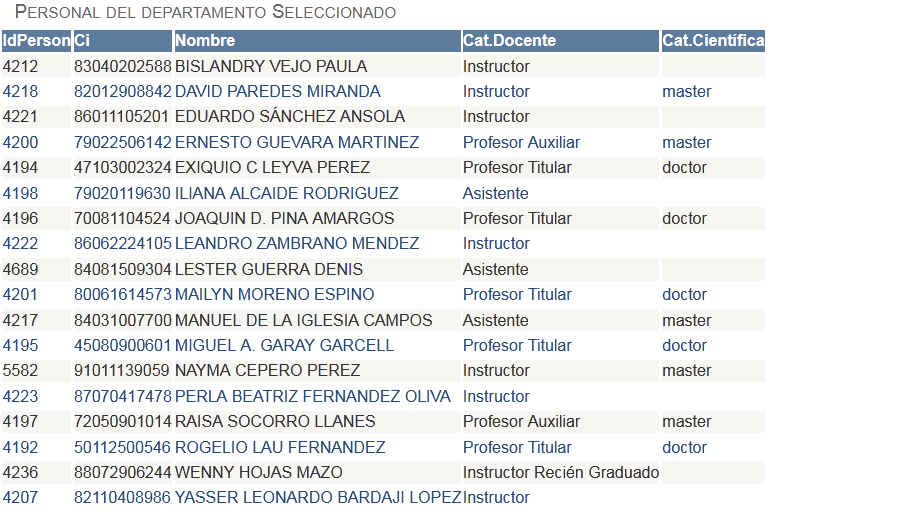
\includegraphics[width=0.9\textwidth]{figuras/catDocCient.png}
	\caption{Información general de los profesores ofrecida por el sistema PANDORA} \label{info-gen-prof}
\end{figure}

\begin{figure} [H]
	\centering
	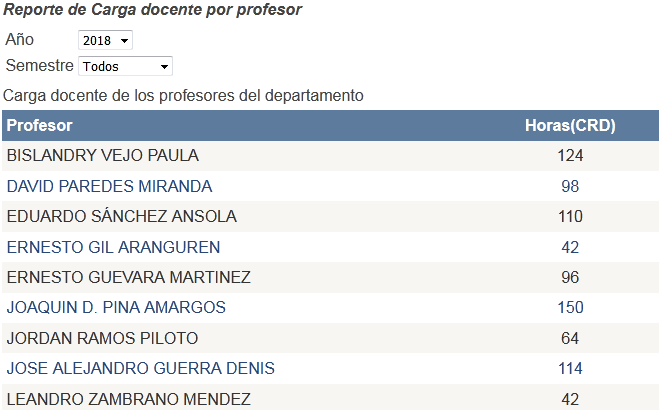
\includegraphics[width=0.7\textwidth]{figuras/HorasProfesor.png}
	\caption{Carga docente de los profesores ofrecida por el sistema PANDORA} \label{horas-prof}
\end{figure}

Además de los datos mostrados anteriormente, se almacenan los años de experiencia y la evaluación anual del profesor. Esta evaluación incluye seis dimensiones: docente, metodológico, investigación, superación, extensión universitaria y política. En dependencia de las evaluaciones en estas dimensiones se le otorga al profesor una evaluación general a criterio del jefe de departamento. Los resultados de las evaluaciones se expresan en cuatro categorías: Excelente, Bien, Regular, Mal y No Evaluar. \\

En la Tabla \ref{norm-datos-carga} se muestra el proceso de normalización de los datos. Para esto, es necesario otorgar valores numéricos a las categorías docentes, científicas y a las evaluaciones (tanto anual como general). 

\begin{table} [H]
	\centering
	\caption{Normalización de los datos} \label{norm-datos-carga}
	\begin{tabular}{|c|c|c|}
		\cline{2-3}
		             \multicolumn{1}{c|}{}               &    \textbf{Categorías}     & \textbf{Puntuación} \\ \hline
		 \multirow{5}{3cm}{\textbf{Categoría Docente}}   &      Profesor Titular      &         1.0         \\ \cline{2-3}
		                                                 &     Profesor Auxiliar      &         0.8         \\ \cline{2-3}
		                                                 &         Asistente          &         0.6         \\ \cline{2-3}
		                                                 &         Instructor         &         0.4         \\ \cline{2-3}
		                                                 & Instructor recién graduado &         0.2         \\ \hline\hline
		\multirow{3}{3cm}{\textbf{Categoría Científica}} &  Doctor en Ciencia (Dr. C.)  &         1.0         \\ \cline{2-3}
		                                                 & Máster en Ciencia (MSc.)  &         0.5         \\ \cline{2-3}
		                                                 &          Ninguna           &         0.0         \\ \hline\hline
		     \multirow{5}{3cm}{\textbf{Evaluación}}      &         Excelente          &         1.0         \\ \cline{2-3}
		                                                 &            Bien            &         0.8         \\ \cline{2-3}
		                                                 &          Regular           &         0.6         \\ \cline{2-3}
		                                                 &            Mal             &         0.4         \\ \cline{2-3}
		                                                 &       No Evaluado        &         0.0         \\ \hline
	\end{tabular}
\end{table}

Se propone entonces, a partir de lo planteado en la la Tabla \ref{norm-datos-carga}, las siguientes formulaciones para el cálculo de las competencias técnicas establecidas en las Sección \ref{conjuntos-docente}:

\begin{flalign}
t_1 = c_d&& \label{ec:cat-doc}\\
t_2 = c_c&&\label{ec:cat-cient}\\
%t_3 = \dfrac{A_i}{T}&&\label{ec:exp-prof}\\
t_4 = e_d&&\label{ec:eval-doc}\\
t_5 = e_m&&\label{ec:eval-met}\\
t_6 = e_i&&\label{ec:eval-inv}
\end{flalign}

\vspace{3cm}
Donde:
\begin{description}
	\setlength\itemsep{0em}
	\item[(\ref{ec:cat-doc})] $c_d$ corresponde al valor de la categoría docente normalizado.
	\item[(\ref{ec:cat-cient})] $c_c$ corresponde al valor de la categoría  científica normalizado.
%	\item[(\ref{ec:exp-prof})] $A_i$ años de experiencia del profesor y $T$ es una constante que sería en máximo número de años de experiencia que puede tener una persona.
	\item[(\ref{ec:eval-doc})] $ e_d $ es el valor normalizado de la evaluación docente.
	\item[(\ref{ec:eval-met})] $ e_m $ es el valor normalizado de la evaluación metodológica.
	\item[(\ref{ec:eval-inv})] $ e_i $ es el valor normalizado de la evaluación investigativa.
\end{description}

%(\ref{ec:cat-cient}) $c_c$ corresponde al valor de la categoría  científica normalizada.\\ \vspace{0.3cm}
%(\ref{ec:exp-prof}) $A$ años de experiencia del profesor y $T$ es una constante que sería en máximo número de años de experiencia que puede tener una persona.\\
%(\ref{ec:eval-doc}) $ e_d $ es el valor normalizado de la evaluación docente.\\
%(\ref{ec:eval-met})$ e_m $ es el valor normalizado de la evaluación metodológica.\\
%(\ref{ec:eval-inv}) $ e_i $ es el valor normalizado de la evaluación investigativa.\\

\vspace{0.3cm}
{\color{red}Además, se propone para calcular la experiencia de los profesores en los roles la Fórmula \ref{ec:exp-pers}, mientras que para calcular la preferencia de los profesores por los roles la Fórmula \ref{ec:pref-pers}. Es importante resaltar que  el valor de $X$ en la Fórmula \ref{ec:pref-pers} es un valor configurable por el usuario, al cual se le llamará punto de corte.}
\begin{flalign}\label{ec:exp-pers}
C_i= \left\{ 
\begin{array}{lcl}
\displaystyle{\frac{E_i}{T_i}} & \mbox{ si } & E_i < T_i \\
&             &  \\
1.0 & \mbox{ si } & E_i >=10
\end{array}
\right.&&
\end{flalign}

\begin{flalign}\label{ec:pref-pers}
P_i= \left\{ 
\begin{array}{lcl}
1 & \mbox{ si } & \displaystyle{\frac{E_i}{T_i}} >= X \\
&             &  \\
0 & \mbox{ si } & \displaystyle{\frac{E_i}{T_i}} < X
\end{array}
\right.&&
\end{flalign}

\vspace{0.3cm}
Donde:
\begin{itemize}
	\setlength\itemsep{0em}
	\item $C_i$ el valor de experiencia del profesor en el rol  $i$.
	\item $P_i$ el valor de preferencia del profesor por el rol $i$.
	\item $E_i$ años de experiencia del profesor en el rol $i$.
	\item $T$ años de experiencia del profesor.
	\item $X$ valor definido por el usuario.
\end{itemize}

\vspace{0.5cm}

Para probar las formulaciones planteadas anteriormente, se utilizarán datos ficticios. En las Tablas \ref{datos-prof1} y  \ref{datos-prof2} se muestra la información necesaria de los profesores. Utilizando el modelo planteado, se obtienen los resultados de la Tabla \ref{result-prof} para las competencias técnicas. La Tabla \ref{exp-prof}  visualiza los años de experiencia de cada profesor impartiendo cada tipo de clases, mientras que la Tabla \ref{trans-prof} refleja la preferencia de los profesores por cada tipo de clases.

\begin{table}[H]
	\centering
	\caption{Datos de los profesores}\label{datos-prof1}
%	\{-2cm}
\scalebox{.9}{
		\begin{tabular}{l c c c }
			\toprule[1.7pt]
		Profesor(a) & Categoría Docente  & Categoría Científica & Años experiencia \\ \midrule
			Raisa Socorro                             & Profesora Auxiliar & Doctor               & 24               \\
		\rowcolor{gray!30}	Joaquín Pina                              & Profesor Titular   & Doctor               & 25               \\
			Alejandro Rosete                          & Profesor Titular   & Doctor               & 25               \\
			\bottomrule[1pt]            
		\end{tabular}
	}
\end{table}

\begin{table}[H]
	\caption{Evaluación de los profesores}\label{datos-prof2}
	\centering
%	\hspace{-2cm}
\scalebox{.9}{
	\begin{tabular}{l c c c}
		\toprule[1.7pt]
		Profesor(a) & Trabajo docente & Trabajo metodológico & Trabajo investigativo \\ \midrule
		Raisa Socorro                             & Excelente       & Excelente            & Bien                  \\
		\rowcolor{gray!30} Joaquín Pina                              & Excelente       & Bien                 & Bien                  \\
		Alejandro Rosete                          & Excelente       & Excelente            & Excelente             \\
	\bottomrule[1pt]        
	\end{tabular}
		}
\end{table}




\begin{table}[H]
	\centering
	\caption{Resultado de la transformación de las competencias técnicas de los profesores}\label{result-prof}
%	\hspace{-2cm}
\scalebox{.9}{
	\begin{tabular}{l c c c}
		\toprule[1.7pt]
		Competencias técnicas & Raisa Socorro & Joaquín Pina & Alejandro Rosete \\ \midrule
		$t_1=categor\acute{\i}a\;docente$                   & 0.8           & 1.0          & 1.0              \\
		$t_2=grado\;cient\acute{\i}fico$                    & 1.0           & 1.0          & 1.0              \\
		$t_4=trabajo\;docente$                              & 1.0           & 1.0          & 1.0              \\
		$t_5=trabajo\;metodol\acute{o}gico$                 & 1.0           & 0.8          & 1.0              \\
		$t_6=trabajo\;investigativo$                        & 0.8           & 0.8          & 1.0              \\
		\bottomrule[1pt]                     
	\end{tabular}
}
\end{table}

\begin{table}[H]
	\centering
	\caption{Años de experiencia de los profesores}\label{exp-prof}
	\scalebox{.9}{
	\begin{tabular}{l c c c c c c}
		\toprule[1.7pt]
		Profesor(a) & C  & CP & S  & L  & T & JA \\ \midrule
		Raisa Socorro                             & 20 & 10 & 2  & 0  & 2 & 4  \\
		\rowcolor{gray!30} Joaquín Pina                              & 20 & 15 & 12 & 10 & 2 & 5  \\
		Alejandro Rosete                          & 19 & 14 & 7  & 0  & 1 & 10 \\
		\bottomrule[1pt]            
	\end{tabular}
}
\end{table}

A continuación se explica, cómo se pueden calcular las preferencias de las profesores por los roles utilizando la Fórmula \ref{ec:pref-pers} y los datos de los profesores presentados en las Tablas \ref{datos-prof1} y \ref{exp-prof}. Por ejemplo, en el caso del profesor Joaquín Pina (cuyos datos están resaltados en gris en las tablas), al tener diez años de experiencia o más en los roles: C, CP, S, y L, el grado de preferencia por cada uno de ellos es el mismo: 1.0. Sin embargo, su experiencia en los roles T y JA es menor de diez años, por lo que al normalizarlos, se obtienen los valores para el grado de preferencia para estos roles de $0.2$ y $0.5$. En la Tabla \ref{trans-prof} se muestran los resultados para todos los profesores cuyos datos están disponibles en las Tablas \ref{datos-prof1} y \ref{exp-prof}.


\begin{table}[H]
	\centering
	\caption{Transformación de los años de experiencia a la preferencia de los profesores por los roles}\label{trans-prof}
	\scalebox{.9}{
	\begin{tabular}{l c c c c c c}
		\toprule[1.7pt]
		Profesor(a) & C   & CP  & S   & L   & T   & JA  \\ \midrule
		Raisa Socorro                             & 1.0 & 1.0 & 0.2 & 0.2 & 0.2 & 0.4 \\
		\rowcolor{gray!30} Joaquín Pina                              & 1.0 & 1.0 & 1.0 & 1.0 & 0.2 & 0.5 \\
		Alejandro Rosete                          & 1.0 & 1.0 & 0.7 & 0.0 & 0.1 & 1.0 \\
		\bottomrule[1pt]          
	\end{tabular}
}
\end{table}

\section{Diseño de la solución propuesta} \label{sec:diseno-solucion}

Esta sección tiene como objetivo, describir la propuesta para la importación de los datos provenientes de un fichero, en datos que gestiona la herramienta TEAMSOFT$^+$. Para lograr esto, se muestran los artefactos de ingeniería de software necesarios para entender su funcionamiento, como son: diagrama de casos de uso del sistema y diagrama de paquetes.


\subsection{Proceso propuesto para importar datos desde la herramienta TEAMSOFT$^+$}
Esta sección se comprueba el correcto funcionamiento de las nuevas funcionalidades incorporadas a la herramienta TEAMSOFT$^+$ vinculadas con el proceso de importación de personas. En la Figura \ref{fig:diagrama-flujo-importar} se presenta el diagrama de flujo asociado a este proceso. 

\begin{figure}[H]
	\centering
	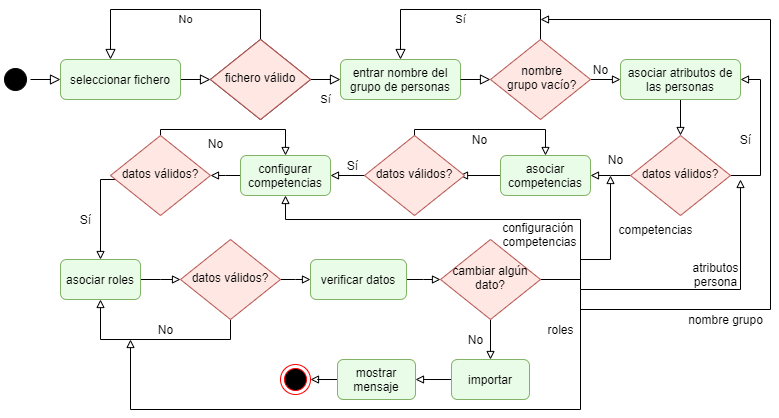
\includegraphics[width=.85\textwidth]{figuras/diagramas-teamsoft-Flujo-Importar.png}
	\caption{Diagrama de flujo para representar la importación de datos	} \label{fig:diagrama-flujo-importar}
\end{figure}

El proceso comienza cuando el usuario \textbf{selecciona un fichero} a importar. Este fichero tiene que cumplir las características que se listan en la Tabla \ref{table:especificaciones-fichero}. Este formato permite que la información almacenada en el fichero se adapte a diferentes tipos de problemas.

\begin{table}[H]
	\centering
	\caption{Especificaciones del fichero a importar}\label{table:especificaciones-fichero}
	\begin{tabular} {l | p{10cm}}
		\toprule
		Formato & Valores separados por comas o \textit{CSV}, por sus siglas en inglés (\textit{.csv}) \\ \midrule
		Composición & Cada columna representa un atributo de las personas. Mientras que cada fila representa los valores de las personas en cada atributo. \\ \hline
		Campos obligatorios & La experiencia y el nombre de las personas \\ \hline
		Campos adicionales & Todos los atributos relacionados con el problema en cuestión \\ \hline 
		Restricciones & El tipo de dato de cada columna tiene que ser homogéneo \\ \bottomrule
	\end{tabular}
\end{table}

En el paso entrar nombre del grupo de personas, el usuario selecciona de los grupos disponibles, a cuál de ellos incorporar las personas a importar. En caso de no existir el grupo deseado, este se crea al finalizar el proceso, justo antes de insertar a las personas. A continuación es necesario asociar las características de las personas disponibles en el fichero de entrada a los atributos de las personas definidos, para esto deben coincidir los tipos de datos. De forma similar, se definen los atributos del fichero a partir de los cuáles se calculan los valores de las competencias utilizando las ecuaciones definidas en las secciones \ref{sec:tran_pel} y \ref{sec:tran_docencia}. En el siguiente paso es necesario establecer los pesos asociados a cada una de las categorías de las competencias. Existen diferentes criterios para determinar estos pesos, en función del tipo de dato de los atributos en el fichero de entrada que influyen en las competencias definidas en el paso anterior. Antes de finalizar el proceso, se mapean los atributos del fichero con los roles correspondientes. En este momento es posible comprobar las configuraciones realizadas, y decidir entonces finalizar el proceso de importación o modificar alguno de los pasos anteriores. \\

Durante todo el proceso es posible además, establecer una configuración que se tiene en cuenta a la hora de importar. En esta, se le permite al usuario decidir qué acción realizar ante la existencia en el sistema de personas que ya fueron importadas. Para esta opción, el usuario debe decidir si desea ignorar las personas existentes (no las inserta) o actualizar sus valores (dígase niveles en las competencias y preferencias por los roles). En adición, si se marca la opción de actualización de los datos, aparece una nueva opción. Esta nueva opción permite decidir entre mantener los valores viejos que no se actualizan y añadir los nuevos o, simplemente, borrar los viejos y añadir los nuevos. Otros parámetros configurables son: el número de años de experiencia de una persona para considerar que tiene el máximo y, el punto de corte para determinar la preferencia de la persona por un rol. \\

En función de las configuraciones establecidas, durante el proceso de importación se realizan las operaciones de inserción, eliminación o actualización de los datos. Estas operaciones se realizan en las siguientes tablas de la base de datos:
\begin{description}
	\item[worker:] se almacenan los datos de las personas como el nombre, la experiencia y el grupo al que pertenecen.
	\item[person\_group:] guarda la información relativa a los grupos que pertenecen las personas.
	\item[competence\_value:] almacena los niveles de las personas en las competencias. 
	\item[personal\_interest] guarda la información relacionada con los intereses de las personas por los roles 
	\item[role\_experience:] almacena la experiencia de la persona en los roles.
\end{description}

\subsection{Descripción del diseño de la solución propuesta}

En esta sección se muestran los artefactos de ingeniería de software necesarios para entender y explicar el funcionamiento de la funcionalidad de importar el fichero.

\subsubsection{Diagrama de casos de uso}

La funcionalidad a implementar se relaciona con la incorporación de personas, roles y competencias. Es por este motivo que se decide que el responsable de llevarlas a cabo sea el rol \textbf{Gestor de recursos humanos}. Debido a la gran número de CU que posee el sistema, se decide mostrar solamente aquellos que fueron modificados o creados por el autor. En la Figura \ref{fig:CU_nuevo} se muestra el diagrama el diagrama de CU correspondiente. El color verde corresponde a los CU no modificados, el amarillo a los modificados y el color rojo corresponde a los CU incorporados.

\begin{figure}[H]
	\centering
	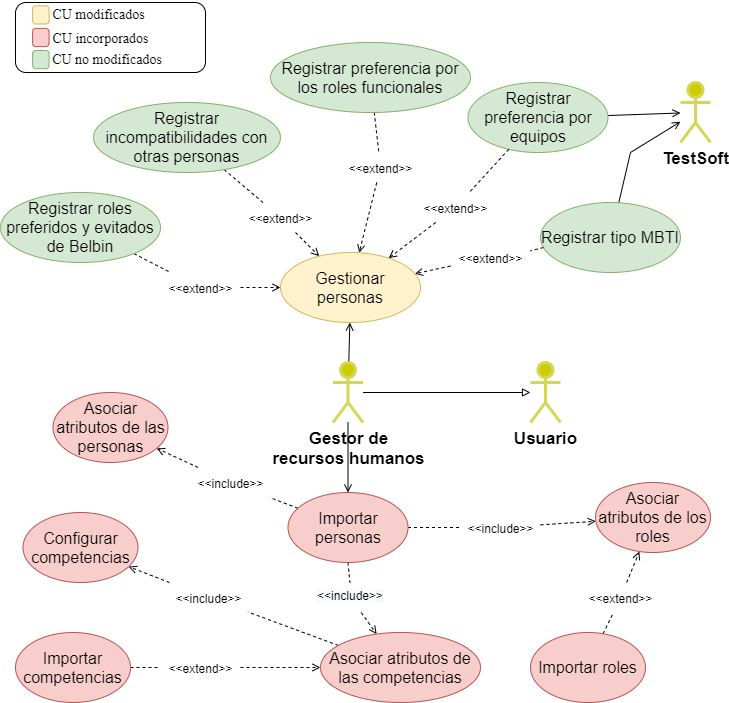
\includegraphics[width=.81\textwidth]{figuras/diagrama_CUTeamSoftImportar.png}
	\caption{Ampliación de diagrama de CU} \label{fig:CU_nuevo}
\end{figure}

\subsubsection{Descripción de alto nivel de los casos de uso}
En esta sección se describen cada uno de los casos de uso relacionadas con la funcionalidad a implementar. En cada uno se explican elementos tales como: el nombre, la descripción y los casos de uso relacionados.\\

La Tabla \ref{table:descripcion-alto-nivel-importar} muestra la descripción de alto nivel del CU Importar Personas.

\begin{table}[H]
	\centering
	\caption{Descripción de alto nivel del CU Importar Persona} \label{table:descripcion-alto-nivel-importar}
	\begin{tabular}{ | l | p{10cm} |}
		\toprule
		Nombre & Importar Personas \\ \midrule
		Descripción & Este es el CU principal de la funcionalidad propuesta. Para importar las personas el usuario debe seleccionar la opción de importar, luego el sistema le muestra una ventana donde debe localizar el archivo que desea importar. Si el fichero posee las características correctas se procede a leer el fichero. Además debe seleccionar (o crear) un grupo al cual asociar las personas a importar.\\ \hline
		CU relacionados & Asociar atributos de las personas, Asociar atributos de las competencias, Asociar atributos de los roles.\\ \bottomrule
	\end{tabular}
\end{table}

La Tabla \ref{table:descripcion-alto-nivel-atr-pers} muestra la descripción de alto nivel del CU Asociar atributos de las personas.

\begin{table}[H]
	\centering
	\caption{Descripción de alto nivel del CU Asociar atributos de las personas} \label{table:descripcion-alto-nivel-atr-pers}
	\begin{tabular}{ | l | p{10cm} |}
		\toprule
		Nombre          & Asociar atributos de las personas                                                                                                                                                \\ \midrule
		Descripción     & En este CU el usuario debe asociar de los atributos del fichero seleccionado, qué elementos corresponden con la experiencia y el nombre de las personas. \\ \hline
		CU relacionados &  \\ \bottomrule
	\end{tabular}
\end{table}

La Tabla \ref{table:descripcion-alto-nivel-atr-comp} muestra la descripción de alto nivel del CU Asociar atributos de las competencias.

\begin{table}[H]
	\centering
	\caption{Descripción de alto nivel del CU Asociar atributos de las competencias} \label{table:descripcion-alto-nivel-atr-comp}
	\scalebox{0.97}{
		\begin{tabular}{ | l | p{10cm} |}
			\toprule
			Nombre          & Asociar atributos de las competencias                                                                                                                                                \\ \midrule
			Descripción     & En este CU el usuario debe asociar a los atributos del fichero que tengan relación con las competencias. Debe especificar todas las competencias que se pueden calcular utilizando este atributo. \\ \hline
			CU relacionados &   Configurar competencias, Importar competencias \\ \bottomrule
		\end{tabular}
	}
\end{table}


La Tabla \ref{table:descripcion-alto-nivel-conf-comp} muestra la descripción de alto nivel del CU Configurar competencias.

\begin{table}[H]
	\centering
	\caption{Descripción de alto nivel del CU Configurar competencias} \label{table:descripcion-alto-nivel-conf-comp}
	\scalebox{0.97}{
		\begin{tabular}{ | l | p{10cm} |}
			\toprule
			Nombre          & Configurar competencias                                                                                                                               \\ \midrule
			Descripción     & En este CU el usuario debe configurar los valores de los atributos relacionados con las competencias. Para esto el usuario debe establecerle a aquellos atributos que contienen campos de texto un valor entre 0 y 1. Un proceso similar debe realizar con aquellos atributos que tienen relación con las mismas competencias. Mientras que para aquellos atributos que almacenan valores numéricos, debe seleccionar el mayor valor presente en el fichero. \\ \hline
			CU relacionados &  \\ \bottomrule
		\end{tabular}
	}
\end{table}

La Tabla \ref{table:descripcion-alto-nivel-imp-comp} muestra la descripción de alto nivel del CU Importar competencias.

\begin{table}[H]
	\centering
	\caption{Descripción de alto nivel del CU Configurar competencias} \label{table:descripcion-alto-nivel-imp-comp}
	\scalebox{0.97}{
		\begin{tabular}{ | l | p{10cm} |}
			\toprule
			Nombre          & Importar competencias                                                                                                                          \\ \midrule
			Descripción     &  Para importar las competencias el usuario debe seleccionar la opción de importar, luego el sistema le muestra una ventana donde debe localizar el archivo que desea importar. Si el fichero posee las características correctas, se procede a leer el fichero.\\ \hline
			CU relacionados &  \\ \bottomrule
		\end{tabular}
	}
\end{table}

La Tabla \ref{table:descripcion-alto-nivel-atr-role} muestra la descripción de alto nivel del CU Asociar atributos de los roles.

\begin{table}[H]
	\centering
	\caption{Descripción de alto nivel del CU Asociar atributos de los roles} \label{table:descripcion-alto-nivel-atr-role}
	\scalebox{0.97}{
		\begin{tabular}{ | l | p{10cm} |}
			\toprule
			Nombre          & Asociar atributos de los roles                                                                                                                              \\ \midrule
			Descripción     & En este CU el usuario debe asociar aquellos atributos del fichero que tengan relación con los roles. Debe especificar para cada atributo seleccionado, el rol que le corresponde. \\ \hline
			CU relacionados & Importar roles \\ \bottomrule
		\end{tabular}
	}
\end{table}


La Tabla \ref{table:descripcion-alto-nivel-imp-role} muestra la descripción de alto nivel del CU Importar roles.

\begin{table}[H]
	\centering
	\caption{Descripción de alto nivel del CU Importar roles} \label{table:descripcion-alto-nivel-imp-role}
	\scalebox{0.97}{
		\begin{tabular}{ | l | p{10cm} |}
			\toprule
			Nombre          & Importar competencias                                                                                                                          \\ \midrule
			Descripción     &  Para importar los roles el usuario debe seleccionar la opción de importar, luego el sistema le muestra una ventana donde debe localizar el archivo que desea importar. Si el fichero posee las características correctas se procede a leer el fichero.\\ \hline
			CU relacionados &  \\ \bottomrule
		\end{tabular}
	}
\end{table}

La Tabla \ref{table:descripcion-alto-nivel-gestion-personas} muestra la descripción de alto nivel del CU Gestionar personas. Este CU como muestra la Figura \ref{fig:CU_nuevo} fue modificado por el autor. La modificación viene dada a partir de una de las limitaciones detectadas en el modelo para el problema de la docencia. El autor añade un nuevo campo a las personas. Este campo consiste en la experiencia profesional de los trabajadores.

\begin{table}[H]
	\centering
	\caption{Descripción de alto nivel del CU Gestionar personas} \label{table:descripcion-alto-nivel-gestion-personas}
	\scalebox{0.97}{
		\begin{tabular}{ | l | p{10cm} |}
			\toprule
			Nombre          & Gestionar personas \\ \midrule
			Descripción     & En este CU el usuario se encarga de crear, modificar, eliminar personas           \\ \hline
			CU relacionados &  \\ \bottomrule
		\end{tabular}
	}
\end{table}

La Tabla \ref{table:descripcion-alto-nivel-restricciones} muestra la descripción de alto nivel del CU Seleccionar restricciones a considerar en la formación de (de los) equipo (s). Este CU fue modificado por el autor. El autor añade nuevas restricciones al problema, y su configuración desde la interfaz de la herramienta.

\begin{table}[H]
	\centering
	\caption{Descripción de alto nivel del CU  Seleccionar restricciones a considerar en la formación de (de los) equipo (s).} \label{table:descripcion-alto-nivel-restricciones}
%	\scalebox{0.97}{
		\begin{tabular}{ | l | p{10cm} |}
			\toprule
			Nombre          &  Seleccionar restricciones a considerar en la formación de (de los) equipo (s).                                                                                                                      \\ \midrule
			Descripción     & El usuario selecciona en función de las características del problema el conjunto de restricciones asociadas. \\ \hline
			CU relacionados & Seleccionar factores a considerar en la formación del (de los) equipos \\ \bottomrule
		\end{tabular}
%	}
\end{table}


En la Figura \ref{fig:diagrama-paquetes-modificado} se muestra una ampliación del diagrama de estructuración en capas de TEAMSOFT$^+$, mostrando solamente los paquetes que  fueron modificados por el autor.

\begin{figure}[H]
	\centering
	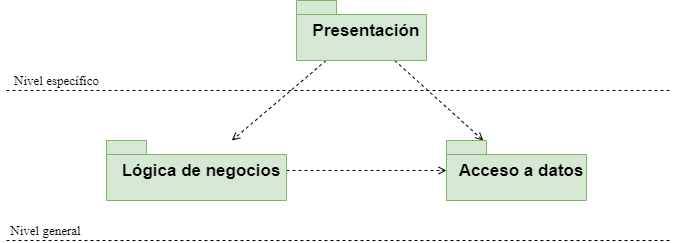
\includegraphics[width=.7\textwidth]{figuras/diagrama-paquetes-modificado.png}
	\caption{Diagrama de estructuración en capas basado en reutilización} \label{fig:diagrama-paquetes-modificado}
\end{figure}

En el paquete de \textbf{Presentación} se incorporan todos las páginas \textit{XHTML (Facelets)} insertadas para la incorporación de la funcionalidad. Además, en el paquete \textbf{Lógica de negocio} se añaden las clases controladoras, útiles y, las clases relacionadas con la solución al modelo de formación de múltiples equipos con la biblioteca BiCIAM. Mientras que en el paquete \textbf{Acceso a datos} se insertaron algunas clases y métodos relacionadas con el acceso a los datos (creación/modificación/eliminación) relacionados con el proceso de importación.\\

Las modificaciones realizadas al CU descrito en la Tabla \ref{table:descripcion-alto-nivel-restricciones}, implicó añadir nuevas restricciones al modelo de formación de equipos múltiples. Estas modificaciones se relacionan con las características propias de cada problema y las limitaciones detectadas cuando se trataba de adapatar cada uno de ellos. Se añadieron dos clases: \textit{BossNeedToBeAssignedToAnotherRole} y \textit{MinimumRoles}. La Figura \ref{fig:diagrama-clases-modificado} muestra un fragmento del diagrama de clases de TEAMSOFT$^+$ al cual se le incorporan dos nuevas clases. La clase \textit{BossNeedToBeAssignedToAnotherRole} modela que la persona que ocupa el rol de Líder tiene que desempeñar al menos otro rol. Mientras que \textit{MinimumRoles} se encarga de que todos los miembros del equipo juegue una cantidad mínima obligatoria de roles. 

\begin{figure}[H]
	\centering
	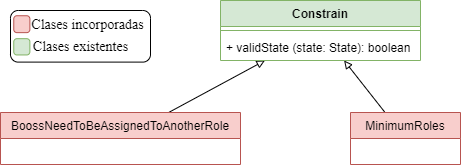
\includegraphics[width=.7\textwidth]{figuras/diagramas-clases-a-incorporar.png}
	\caption{Fragmento del Diagrama de clase de TEAMSOFT$^+$ para incorporar nuevas restricciones} \label{fig:diagrama-clases-modificado}
\end{figure}

{\color{red}
Se plantea añadir la restricción \textit{MinimumRoles} ya que en el béisbol, los jugadores tienen obligatoriamente un rol a la ofensiva y otro a la defensiva. El Algoritmo \ref{alg:rest-min-roles} muestra el pseudocódigo utilizado para la construcción de esta restricción. En cada equipo se verifica que una persona asignada a un rol, también esté asignada a otro rol compatible con este. Se exceptúa de esta restricción al Capitán del equipo (Líder) ya que este puede no formar parte de la alineación inicial. \\

En los equipos docentes es común que el Jefe de asignatura (Líder) forme parte del claustro que la imparte. La restricción \textit{BossNeedToBeAssignedToAnotherRole} verifica que se cumpla esta condición. El Algoritmo \ref{alg:restr-lider-rol} muestra el pseudocódigo utilizado para implementar esta restricción. En este caso para cada equipo se verifica que el Líder esté presente en al menos otro rol. } \vspace{1cm}

\begin{algorithm}[H]
	\caption{Restricción que verifica que una persona no pueda desempeñar menos roles que los definidos}
	%	\SetKwProg{Sol}{Restricci}{}{}
	\label{alg:rest-min-roles}
	%\Sol{($projects$)}{
	\KwIn {$state$ \tcp*[l]{estado que contiene los proyectos a verificar}
		\hspace{1.7cm}        $minRoles$ \tcp*[l]{Número obligatorio de roles a desempeñar} }
	\KwOut {$isRight$ \tcp*[l]{si todos los proyectos cumplen con la restricción}}
	%\LinesNumbered
	$projects = state$.getCode()\;
	$isRight = true$\;
	
	\ForEach{$project \in projects$}
	{$projectRoles = project$.getRoles() \tcp*[l]{roles del proyecto}
		projectRoles.remove(projectRoles.getBoss()) \tcp*[l]{se elimina al jefe}
		\ForEach{$rol \in projectRoles$}
		{
			$roleWorkers = rol$.getWorkers() \tcp*[l]{personas asociadas al rol}
			\ForEach{$worker \in roleWorkers$}
			{
				\If{$project$.getCantOccurenceWorker($worker$) $< minRoles$}{
					$isRight = false$ \tcp*[l]{no cumple con la restricción}
					\Break
				}
			}
			\If{$!isRight$} \Break
		}
		\If{$!isRight$} \Break
	}
	\Return $isRight$
	%}
\end{algorithm} \vspace{1cm}

En la Sección \ref{sec:teamsoft} se mencionó que TEAMSOFT$^+$ utiliza los algoritmos metaheurísticos implementados en la biblioteca de  BiCIAM para dar solución al problema de formación de equipos. Para que estos algoritmos trabajen, deben partir de una solución inicial del problema. La construcción de la solución inicial es la forma en que la herramienta accede al espacio de búsqueda y selecciona las personas para asignarlas a los equipos. Es importante recordar que se parte de la solución inicial creada, lo que implica formar los equipos requeridos, para después buscar mejorarlos aplicando operadores. Así, la calidad de la solución de un problema heurístico depende en gran parte de la construcción de la solución inicial y de qué tan buenos sean los operadores empleados.\\


\begin{algorithm}[H]
	\caption{Restricción que verifica que el Líder del equipo ocupa otro rol como mínimo en el mismo equipo}
	\label{alg:restr-lider-rol}
	\KwIn {$state$ \tcp*[l]{estado que contiene los proyectos a verificar}}
	\KwOut {$isRight$ \tcp*[l]{si todos los proyectos cumplen con la restricción}}
	%\LinesNumbered
	$projects = state$.getCode()\;
	$isBossAssignedMoreThanOnce = false$\;
	\ForEach{$project \in projects$}
	{
		$isBossAssignedMoreThanOnce = false$\;
		$projectRoles = project$.getRols() \tcp*[l]{roles del proyecto}
		$roleBoss = project$.getProjectBoss()\;
		$projectRoles$.remove($roleBoss$)\;
		\ForEach{$rol \in projectRoles$}
		{
			$roleWorkers = rol$.getWorkers() \tcp*[l]{personas asociadas al rol}
			\ForEach{$worker \in roleWorkers$}
			{
				\If{$worker$.equals($roleBoss$.getWorkers().get(0))}{ \tcp*[l]{si el worker actual es igual al líder}
					$isBossAssignedMoreThanOnce = true$ \tcp*[l]{si cumple la restricción}
					\Break
				}
			}
			\If{$isBossAssignedMoreThanOnce$} \Break
		}
		\If{$!isBossAssignedMoreThanOnce$} \Break
	}
	\Return $isBossAssignedMoreThanOnce$
	%}
\end{algorithm} \vspace{1cm}

{\color{red}En sus inicios, la herramienta construía la solución inicial de forma aleatoria y utilizaba la estrategia de rechazo para dar tratamiento a las restricciones. Teniendo en cuenta que la formación de equipos puede incluir muchas restricciones, una gran cantidad de soluciones se rechazaban porque resultaban no factibles (incumplir al menos una restricción). Esto implicaba pérdida de tiempo en la construcción de una solución inicial. En \cite{Duran2019} se incorporan a la herramienta dos formas de construcción de la solución inicial tomando en cuenta las restricciones más incumplidas hasta ese momento: las competencias y los roles de Belbin.}\\

{\color{red}En la formación de equipos docentes, al utilizar las construcciones iniciales incorporadas, se generan una gran cantidad de soluciones no factibles si se tienen en cuenta la restricción de que el jefe de la asignatura debe formar parte del claustro. Ante esta situación, se agrega una nueva construcción inicial que tenga en cuenta esta restricción. El Algoritmo \ref{alg:const-lider-rol} se presenta el pseudocódigo propuesto, donde después de realizada la asignación de las personas a los roles de forma aleatoria, se selecciona una persona entre las ya asignadas para ocupar el rol de Líder.} \\

\scalebox{.88}{
	\begin{algorithm}[H]
		\caption{Asignar personas de forma aleatoria a los roles, estableciendo que el líder juega más de un rol en los equipos}
		\label{alg:const-lider-rol}
		%\Sol{($projects$)}{
		\KwIn {$projects$ \tcp*[l]{Lista de proyectos sin asignación inicial}
			\hspace{1.7cm}        $limitPersonTries$ \tcp*[l]{Número de intentos de poner una persona en un rol} }
		\KwOut {$projects$ \tcp*[l]{Lista de proyectos con asignación inicial}}
		%\LinesNumbered
		\ForEach{$project \in projects$}
		{$rols = project$.getRoles() \tcp*[l]{roles del proyecto}
			$rols$.remove($boss = project$.getProjectBoss()\;
			\ForEach{$rol \in rols$}
			{$needs=rol$.getNeedWorked()\tcp*[l]{trabajadores necesarios en el rol}
				$count = 0$\;
				\While{$(needs > 0) \And (count < limitPersonTries)$}
				{
					$chosenPerson=$randomPersons()\tcp*[l]{seleccionar aleatoriamente una persona}
					\If{checkIndividualRestrictions($chosePerson,rol$)}
					{$rol=$.getWorkers().add(chosenPerson)\tcp*[l]{se añade si cumple las restricciones}
						$needs--$\;}
					\Else
					{
						$count++$\;}
				}
			}
			$rol$ = getRandomRol($rols$)\tcp*[l]{selecciona un Rol aleatoriamente}
			$worker$=getRandomWorker($rol$.getWorkers())\tcp*[l]{selecciona aleatoriamente un trabajador asignado a ese Rol}
			$boss$.getWorkers().add($worker$)\tcp*[l]{A ese trabajador se asigna el rol de Líder}
			$rols$.add($boss$)\;
		}
	\end{algorithm} \vspace{1cm}
}

En el caso del béisbol las soluciones iniciales generadas aún utilizando las soluciones iniciales incorporadas por \cite{Duran2019} generan un gran número de soluciones no factibles, ya que no tienen en cuenta las incompatibilidades entre los roles ni la restricción \textit{MinimumRoles}. En este trabajo se propone la construcción de una solución inicial como la descrita en el Algoritmo \ref{alg:2}. En este algoritmo se asignan todas las personas hasta satisfacer las demandas de los roles teniendo en cuenta las incompatibilidades entre estos. Una vez cubiertos los roles, se elige una personas aleatoria y se establece como Líder. \\

En TEAMSOFT$^+$, con vistas a mejorar las soluciones generadas se utilizan dos operadores de mutación: \textit{performMutation} y \textit{performPermutation}. En el primer caso se realiza un intercambio entre una persona asignada a un rol seleccionado de forma aleatoria y otra persona no asignada. Mientras que en \textit{performPermutation} se realiza la permutación entre dos personas asignadas a dos roles diferentes dentro del equipo, estos roles son seleccionados de forma aleatoria. \\

En los problemas de formación de equipos docentes y de béisbol, el uso de ambos operadores de mutación generan muchas soluciones no factibles. Esto sucede porque no tienen en cuenta las restricciones \textit{MinimumRoles} y \textit{BossNeedToBeAssignedToAnotherRole}. Se incorpora un nuevo operador de mutación \textit{performExternalSubtitution} en el cual se selecciona un rol de forma aleatoria, del cual se sustituye aleatoriamente una persona A por otra B que aún no ha sido asignada. Esta sustitución se realiza además en todos los roles en que ha sido asignada la persona A. En el Algoritmo \ref{alg:operador-sustitucion} se muestra el pseudocódigo para este operador.

\newgeometry{left=1.5cm,right=1.5cm,top=2cm,bottom=.5cm} 
\scalebox{.9}{
	\begin{algorithm}[H]
		\caption{Asignar personas aleatoriamente a roles con la restricción de 2 roles mínimos.}
		%  \SetKwProg{Sol}{SolucionInicial2}{}{}
		\label{alg:2}
		%  %\Sol{($projects$)}{
		\KwIn {$projects$ \tcp*[l]{Lista de proyectos sin asignación inicial}
			\hspace{1.7cm}$limitPersonTries$ \tcp*[l]{Intentos de poner una persona en un rol} 
			%\hspace{1.7cm} $minRolePerson$  \tcp*[l]{Número mínimo de roles que desempeña una persona en un proyecto}
		}
		\KwOut {$projects$ \tcp*[l]{Lista de proyectos con asignación inicial}}
		%\LinesNumbered
		$allWorkers=$getWorkerAvailable()\tcp*[l]{Obtener trabajadores disponibles} 
		\ForEach{$project \in projects$}
		{$rols = project$.GetRols() \tcp*[l]{roles del proyecto}
			$assignedWorkers = {}$\tcp*[l]{ workers asignados con el número mínimo de roles}
			$assignedRoleWorkers= {}$\tcp*[l]{ roles con todos los trabajadores asignados}
			$existWorkers = true$ \tcp*[l]{existen trabajadores disponibles}
			$existCompatibleRole = true$ \tcp*[l]{existen roles compatibles disponibles}
			\tcc{mientras existan disponibilides}		
			\While{$\mbox{\rm existAvailableRoles}(allProjectRoles,assignedRoleWorkers) \And existWorkers$} {
				\tcc{selecciona aleatoriamente un trabajador disponible}
				$workerToAssign =$ getRandomNotAssignedWorker($allWorkers$, $assignedWorkers$)\;
				\If{ $workerToAssign \neq null$} 
				{\tcc{existe un trabajador disponible}
					$roleToAssign = $getRandomAvailableRole($allProjectRoles$, $assignedRoleWorkers$\tcp*[l]{rol con trabajadores por asignar}
					$compatibleRole =$ getRandomCompatibleRole($rols$, $roleToAssign$, $assignedRoleWorkers$)\tcp*[l]{roles compatibles con $roleToAssign$ no asignados}
					\If{$compatibleRole \neq null$} { 
						\tcc{si hay rol compatible asigna el worker a los roles}
						$roleToAssign.$getWorkers().add($workerToAssign$)\;
						$compatibleRole.$getWorkers().add($workerToAssign$)\;
						$assignedWorkers.$add($workerToAssign$)\tcp*[l]{worker asignado}
						\tcc*{los roles satisfacen su demanda de trabajadores})
						\If {$roleToAssign.$getWorkers().size() =$roleToAssign.$getNeededWorkers()}{ 
							$assignedRoleWorkers.$add(roleToAssign)\;}
						\If{$compatibleRole.$getWorkers().size() == $compatibleRole.$getNeededWorkers()} {
							$assignedRoleWorkers.$add($compatibleRole$)\;
						}
					} 
					\Else{$existCompatibleRole = false$\;
					}
				} 
				\Else{$existWorkers = false$\;}
			}
			
			\If{$existWorkers \And existCompatibleRole$} {
				$projectBoss=rol$.getProjectBoss()\;
				
				$boss=$getRandomPerson($allWorkers$)\;
				$projectBoss$.getWorkers().add($boss$);
			}
		}
	\end{algorithm}
}
\restoregeometry 




\begin{algorithm}[H]
	\caption{Operador de sustitución}
	\label{alg:operador-sustitucion}
	\KwIn {$projects$ \tcp*[l]{listado de equipos} \hspace{1.7cm} $codificacion$ \tcp*[l]{configuración del problema}
	}
	\KwOut {lista de proyectos actualizada}
	$randomProject = getRandomProject(projects)$  \tcp*[l]{obtener equipo aleatorio}
	$allProjectRoles = randomProject$.getRoleWorkers()  \tcp*[l]{escoger un rol aleatorio}
	$allWorkers = codification$.getSearchArea()  \tcp*[l]{workers disponibles}
	
	\If{$!allProjectRoles.isEmpty()$}{ 
		$randomRole = getRandomRole(allProjectRoles)$ \;
		$randomWorkerOfSelectedRole = getRandomWorkerByRole(randomRole)$\;
		$workerToSwap=getRandomWorker(allWorkers)$ \;
		\ForEach{$roleWorker \in allProjectRoles$}
		{
			\ForEach{$worker \in roleWorker.getWorkers()$}
			{
				\If{$worker$.equals($randomWorkerOfSelectedRole$)}{
					$roleWorker$.getWorkers().replace(worker, randomWorkerOfSelectedRole)			\;			
				}			
			}	
		}
	}
\end{algorithm}
 

\section{Conclusiones parciales}
Asignar personas de forma aleatoria a los roles, estableciendo que el líder juega más de un rol en los equipos

Asignar personas aleatoriamente a roles con la restricción de 2 roles mínimos


Con la culminación de este capítulo, se arribaron a las siguientes conclusiones:
\begin{enumerate}
	\item Al incorporar a la herramienta la funcionalidad de importación de datos facilita incorporar de forma rápida los datos almacenados en ficheros externos para dar solución al problemas de formación de equipos.
	\item La herramienta TEAMSOFT$^+$ presenta algunas limitaciones para adaptar los problemas de béisbol y docencia. En el caso del béisbol no se tiene en cuenta que un jugador tiene que jugar dos posiciones compatibles entre sí (una ofensiva y otra defensiva). Mientras que para el caso de la docencia no se tiene en cuenta que en algunas ocasiones el Líder debe formar parte del claustro de la asignatura.
	\item Al incorporar la restricción \textit{BossNeedToBeAssignedToAnotherRole} y la construcción de la solución inicial que asegura que el Líder del equipo ocupe otro rol, es posible aplicar el modelo de formación de  equipos múltiples para formar equipos docentes.
	\item Al incorporar la restricción \textit{MinimumRoles} y la construcción de la solución inicial que asegura que todos los jugadores (excepto el Líder) jueguen dos roles dentro del equipo, es posible aplicar el modelo de formación de  equipos múltiples para formar equipos de béisbol.
\end{enumerate}

	\chapter{Herramienta para la transformación de los datos} \label{chap:3}

Este capítulo tiene como objetivo, describir la propuesta de software para la transformación de los datos existentes en bases de datos conocidas, a los datos que se gestionan en TEAMSOFT$^+$. Para lograr esto, se muestran los artefactos de ingeniería de software necesarios, para entender su funcionamiento, como son: diagrama de casos de uso del sistema, requisitos funcionales y no funcionales. Para finalizar el capítulo se describe la validación de la herramienta presentada. Para esto, se realiza un mapeo entre las tablas de la base de datos utilizadas en dicho sistema, y las tablas que utiliza TEAMSOFT$^+$.

\vspace{0.5cm}

\section{Características de la herramienta}


\paragraph{Requisitos funcionales}
\begin{itemize}
	\item La aplicación debe permitir importar la información de los problemas de béisbol y docentes, almacenada en ficheros externos.
	\item La aplicación debe exportar la información gestionada de manera que TEAMSOFT$^+$ lo pueda incorporar para darle solución al problema.
	\item Editar y visualizar la información importada de los ficheros externos que contienen la información almacenada de los profesores/peloteros.
	\item Insertar los valores necesarios a cumplir por las personas en los roles, competencias.
	\item Establecer las incompatibilidades entre los roles y entre las personas.
\end{itemize}

\paragraph{Requisitos no funcionales}
\begin{itemize}
	\item Los permisos de acceso al sistema podrán ser cambiados solamente por el administrador.
	\item El sistema debe tomar el cuenta las categorías docentes y los tipos de actividades estipuladas en el reglamento docente.
	\item El sistema debe tomar en cuenta las posiciones del juego establecida en el reglamento del béisbol.
	\item El sistema debe proporcionar mensajes de error que sean informativos y orientados al usuario.
	\item El sistema debe poseer una interfaz gráfica amigable.
\end{itemize}

En el sistema interactúan tres tipos de usuarios principales. En la Figura \ref{fig:cu-sistema} se observan estos usuarios, junto con sus respectivos casos de uso.

\begin{figure}[H]
	%	\centering
	\hspace{-0.5cm}
	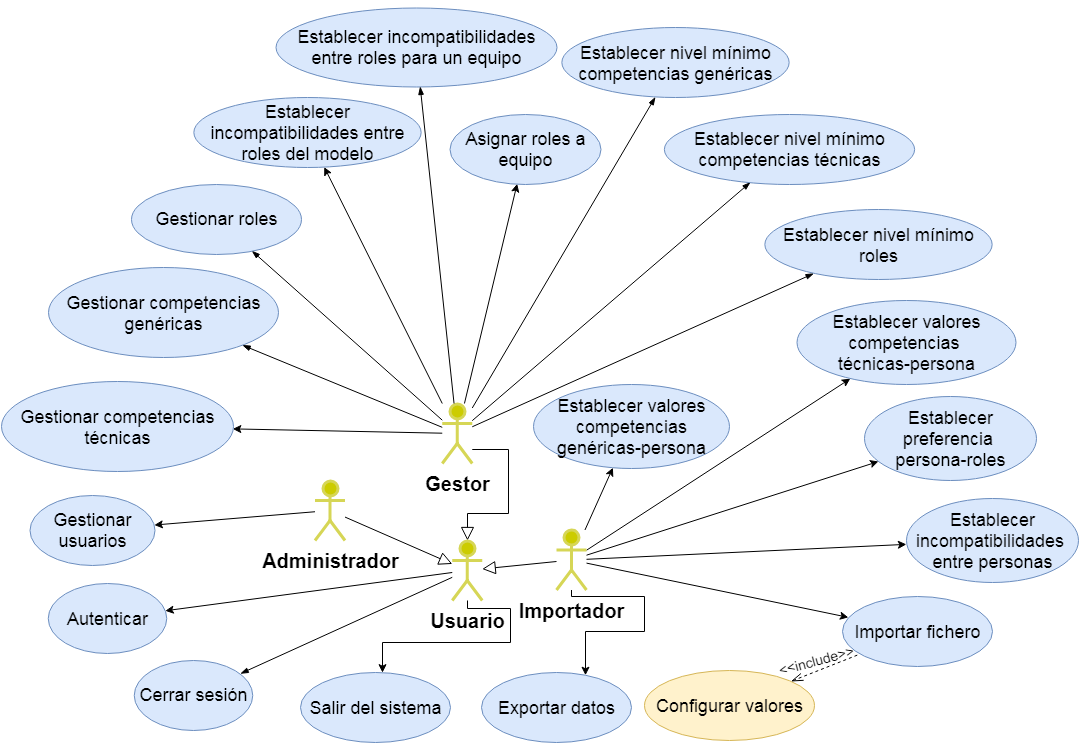
\includegraphics[width=1.1\textwidth]{figuras/DiagramaCUPP3.png}
	\caption{Diagrama de caso de uso del sistema}\label{fig:cu-sistema}
\end{figure}

%\begin{table}[H]
%	\centering
En la Tabla \ref{desc-cu} se muestra para cada caso de uso presente en la Figura \ref{fig:cu-sistema}, la descripción detallada correspondiente.

\begin{longtable}{| c | p{3cm} | p{9cm} |}
	\caption{Descripción de los Casos de Uso}\label{desc-cu}\\
	\toprule[1.7pt]
	\textbf{No.} & \textbf{Caso de Uso} & \textbf{Descripción}\\ \hline
	\endfirsthead
	\multicolumn{3}{c}{\tablename - \thetable\ -- \textit{Continuación de la página anterior} }\\ \toprule[1.2pt]
	\textbf{No.} & \textbf{Caso de Uso} & \textbf{Descripción}\\ \hline
	\endhead
	\multicolumn{3}{r}{\tablename - \thetable\ -- \textit{Continúa en la página siguiente} }\\
	\endfoot
	\endlastfoot
	
	
	CU1&Autenticar & Para poder interactuar con el sistema todos los usuarios deben de autenticarse. Para esto, el usuario en cuestión debe introducir su nombre y contraseña. En función de la existencia del usuario y la correspondencia de la contraseña introducida con la almacenada, se permite que el usuario entre al sistema o, se le muestra un mensaje de error informando lo sucedido.\\ \hline
	
	CU2&Cerrar sesión & Una vez que el usuario se autentica puede cerrar la sesión de trabajo actual. El sistema lanza un mensaje de confirmación, y si el usuario reafirma su decisión entonces es redireccionado a la pantalla de inicio, donde debe de introducir sus credenciales.\\ \hline
	
	CU3&Salir del sistema & Una vez que el usuario se autentica tiene la opción de salir de la aplicación. El sistema lanza un mensaje de confirmación, y en caso de que el usuario reafirme su decisión, se cierra el sistema.\\ \hline
	
	CU4&Gestionar usuarios & Este caso de uso lo desencadena cualquier usuario que esté registrado como \textit{administrador}. En función de la decisión del administrador, puede añadir, editar y eliminar usuarios. En el caso de la adición de usuarios, el decisor deberá de elegir el tipo de problema al cuál pertenecerá el nuevo usuario, así como los roles de este.\\ \hline
	
	CU5&Gestionar competencias genéricas & El caso de uso inicia cuando un usuario registrado como \textit{gestor} requiere añadir o eliminar competencias genéricas. Si desea añadir alguna competencia, es necesario que rellene los datos correspondientes.\\ \hline
	
	CU6&Gestionar competencias técnicas & El caso de uso lo inicia cualquier usuario registrado con el rol de \textit{gestor} que requiera añadir o eliminar competencias técnicas. Si desea añadir alguna competencia, es necesario que rellene los datos correspondientes\\ \hline
	
	CU7&Gestionar roles & Cualquier usuario registrado en el sistema bajo el rol de \textit{gestor}, puede añadir, editar o borrar los roles vinculados al problema al que pertenece el usuario.\\ \hline
	
	CU8&Establecer incompatibilidades entre roles del modelo & En este caso de uso el usuario con el rol de \textbf{gestor}, define las incompatibilidades entre los roles para todos los equipos pertenecientes a un problema (si estas existen). \\ \hline
	
	CU9&Establecer incompatibilidades entre roles para un equipo & Los usuarios registrados con el rol de \textbf{gestor} son los encargados de establecer para cada equipo, específicamente los roles que son incompatibles.\\ \hline
	
	CU10&Asignar roles a equipo & El caso de uso inicia cuando el \textbf{gestor} decide definir los roles que se deben cubrir en cada equipo. Primero se debe de seleccionar el equipo y después en función de los roles existentes, ir añadiendo los que considere necesario. Todos los roles que cuando se hayan añadido se marquen como necesarios, van a estar presentes en todos los equipos.\\ \hline
	
	CU11&Establecer nivel mínimo de competencia genérica & Los usuarios registrados en el sistema bajo el rol de \textbf{gestor} son los encargados de iniciar este caso de uso. Por defecto, el nivel mínimo a cumplir por una persona en una competencia genérica es 0. El usuario en cuestión, tiene la posibilidad de editar este valor para las todas las competencias genéricas.\\ \hline
	
	CU12&Establecer nivel mínimo de competencia técnica & Los usuarios registrados en el sistema bajo el rol de \textbf{gestor} son los encargados de iniciar este caso de uso. Por defecto, el nivel mínimo a cumplir por una persona en una competencia técnica es 0. El usuario en cuestión, tiene la posibilidad de editar este valor para las todas las competencias técnicas.\\ \hline
	
	CU13&Establecer nivel mínimo de preferencia de las personas por los roles & Los usuarios registrados en el sistema bajo el rol de \textbf{gestor} son los encargados de iniciar este caso de uso. Por defecto, el nivel mínimo a cumplir por una persona en un rol es 0. El usuario en cuestión, tiene la posibilidad de editar este valor para las todas los roles.\\ \hline
	
	CU14&Importar fichero & Se inicia cuando se desea cargar la información de nuevas personas. El \textbf{importador} debe elegir el lugar donde se encuentra el fichero que constituye la fuente de datos. Después de seleccionado el fichero, en función del tipo de problema, debe de configurar las constantes que se tienen en cuenta en las ecuaciones para la transformación de los datos.
	\\ \hline
	
	CU15&Exportar datos & Los usuarios que respondan al rol de \textbf{importador}, son los encargados de la exportación de los datos manejados en el sistema hasta el momento. Este usuario debe elegir los equipos y las personas que va a exportar. Estos datos, así como con los que se relacionan, se transforma e introducen en la base de datos de TEAMSOFT$^+$.\\ \hline
	
	CU16&Establecer valores de las competencias-genéricas & Este caso de uso se inicia después que se realizó el proceso de importación al menos una vez con éxito (existan personas importadas). Los usuarios registrados como \textbf{importador} son los encargados de establecer para cada persona, los valores de las competencias genéricas.\\ \hline
	
	CU17&Establecer valores de las competencias-técnicas & Este caso de uso se inicia después que se realizó el proceso de importación, al menos una vez con éxito (existan personas importadas). Los datos mostrados para cada persona son el resultado de las transformaciones pertinentes de los datos provenientes de los ficheros. Los usuarios registrados como \textbf{importador} son los encargados de editar, para cada persona, los valores de las competencias técnicas.\\ \hline
	
	CU18&Establecer preferencia persona-roles & Este caso de uso se inicia después que se realizó el proceso de importación, al menos una vez con éxito (existan personas importadas). Los datos mostrados para cada persona son el resultado de las transformaciones pertinentes de los datos provenientes de los ficheros. Los usuarios registrados como \textbf{importador} son los encargados de editar, para cada persona, los valores de preferencia por cada rol.\\ \hline
	
	CU19&Establecer incompatibilidades entre personas & Este caso de uso se inicia después que se realizó el proceso de importación, al menos una vez con éxito (existan personas importadas). Aquellos usuarios registrados bajo el rol de \textbf{importador} se encargan de asignar cuáles personas son incompatibles entre sí.\\
	\bottomrule[1pt]
\end{longtable}
%	\end{tabular}
%\end{table}

En la Figura \ref{fig:pantalla-principal} se observa el prototipo para la interfaz de la herramienta propuesta, la cual garantiza el cumplimiento de los requisitos funcionales y no funcionales. Por ejemplo, el menú \textit{Usuario}, abarca del CU1 al CU4. En el menú \textit{Configuración problema} se gestionan los casos de uso del CU5 al CU14, mientras que en \textit{E/S} se garantizan del CU15 al CU19.

\begin{figure}[H]
	\centering
	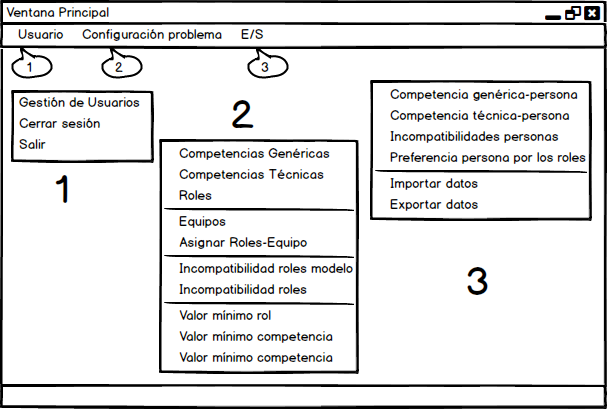
\includegraphics[width=1\textwidth]{figuras/VentanaPrincipal.png}
	\caption{Ventana principal de la aplicación}\label{fig:pantalla-principal}
\end{figure}


En la Figura \ref{fig:diag-clases} se muestra el diagrama de clases utilizado para darle soporte al problema. Para su diseño se tuvieron en cuenta los siguientes aspectos:
\begin{itemize}
	\item En el diagrama se ha creado una clase para cada entidad simple del problema.
	\item La relación de incompatibilidad entre las personas se modela mediante la relación de 0 a muchos entre la clase personas. El extremo 0 indica que una persona puede no tener incompatibilidad con otra persona.
	\item La preferencia de las personas por los roles se muestra en la agregación entre las clases Persona y Rol.
	\item La agregación entre Persona y Problema indica que una persona está disponible para ser asignado a un rol dentro de un equipo para un problema en particular.
	\item Las relaciones de multiplicidad de muchos a muchos, que en el modelo relacional se representan a través de una tabla auxiliar asociativa, en el diagrama de clases solamente se muestran a través de una simple relación de agregación especificando la multiplicidad.
\end{itemize}

\begin{figure}[H]
	\centering
	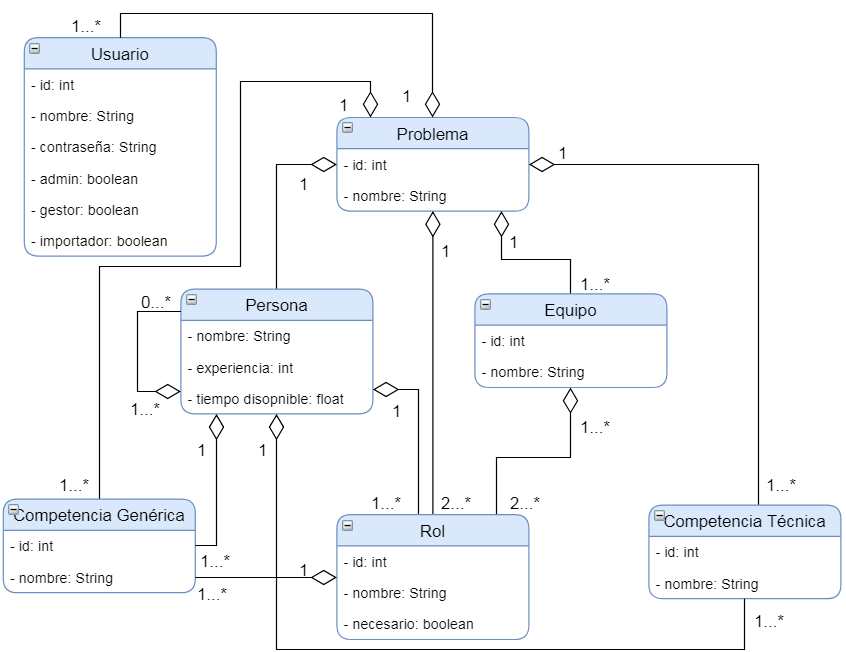
\includegraphics[width=1\textwidth]{figuras/diagramaClases.png}
	\caption{Diagrama de clases}\label{fig:diag-clases}
\end{figure}

En la Figura \ref{fig:estruct-fichero} se muestra la estructura que tienen los ficheros a importar por el sistema para cada tipo de problema. El formato del fichero utilizado fue \textit{csv}, debido que es fácil de editar desde cualquier editor de texto y ocupa poco espacio. Cada fila del fichero almacena la información de una persona. Para cada persona se guardan además de sus estadísticas, la experiencia acumulada en cada rol. Puede verse un ejemplo en la Figura \ref{fig:ejemplo-estruct-fichero} (son los mismos datos utilizados para poblar las Tablas \ref{estadistica-of}, \ref{estadistica-def}, \ref{exp-of} y \ref{exp-def}).

\begin{figure}[H]
	\centering
	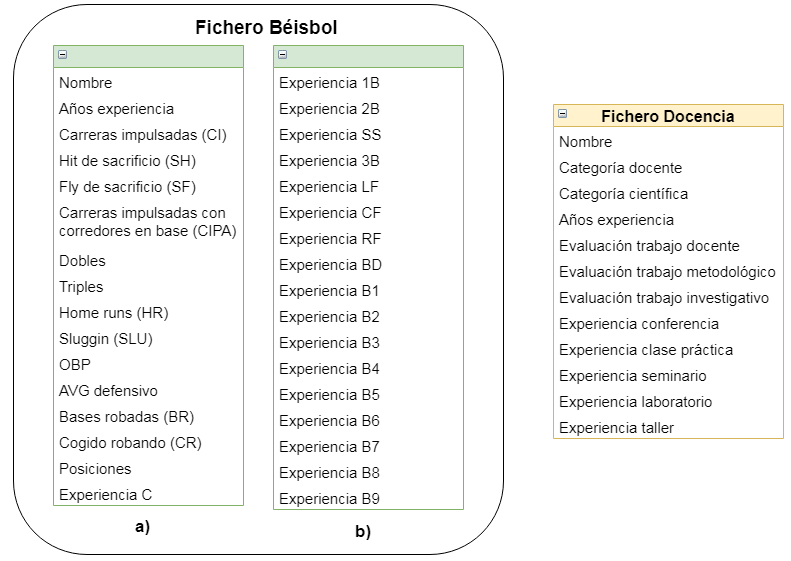
\includegraphics[width=1\textwidth]{figuras/estructuraFichero.png}
	\caption{Estructura de los ficheros}\label{fig:estruct-fichero}
\end{figure}

\begin{figure}[H]
	\centering
	\subfigure[Fichero de béisbol \label{fig:fichero-beisbol}]{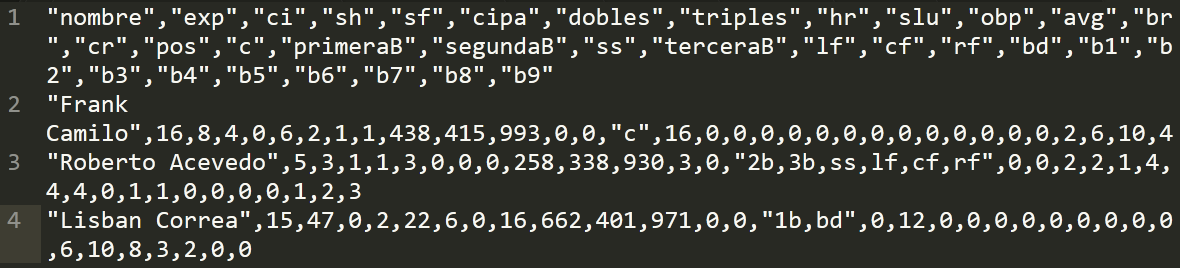
\includegraphics[width=1\textwidth]{figuras/ejemploFicheroPelota.png}}
	\subfigure[Fichero de docencia \label{fig:fichero-docencia}]{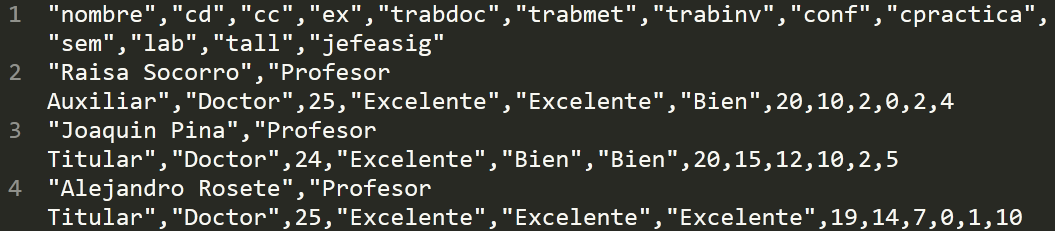
\includegraphics[width=1\textwidth]{figuras/ejemploFicheroDocente.png}}
	
	\caption{Estructura de los ficheros}\label{fig:ejemplo-estruct-fichero}
\end{figure}

\section{Validación de la herramienta}

La herramienta desarrollada en este trabajo gestiona la información pertinente a los problemas de conformación de equipos de béisbol y docencia. Además, el proceso de exportación crea un puente entre los datos, y la posibilidad de conformar equipos con TEAMSOFT$^+$. En esta sección se comprueba el correcto funcionamiento de la herramienta a través de los procesos de importación y exportación, casos de usos CU14 y CU15 descritos en la Tabla \ref{desc-cu}.

\subsection{Importación de los datos}

El usuario que responde al rol de importador debe elegir el lugar donde se encuentra el fichero que constituye la fuente de datos para el tipo de problema. Además, debe de configurar las constantes que se tienen en cuenta en las ecuaciones para la transformación de los datos. En la Figura \ref{fig:conf-constantes} se pueden ver los valores de las constantes utilizadas durante el proceso de importación. El resultado de este proceso, permite obtener de forma automática el grado de preferencia de las personas por los roles, y el valor que tienen las personas en cada una de las competencias técnicas asociadas al problema. \\

\begin{figure} [H]
	\centering
	\subfigure[\label{e}]{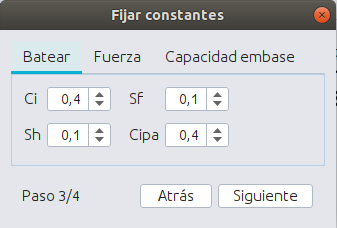
\includegraphics[width=0.45\textwidth]{figuras/fijarConstantes1.png}}
	\subfigure[\label{s}]{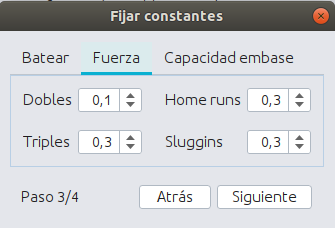
\includegraphics[width=0.45\textwidth]{figuras/fijarConstantes2.png}}
	\subfigure[\label{f}]{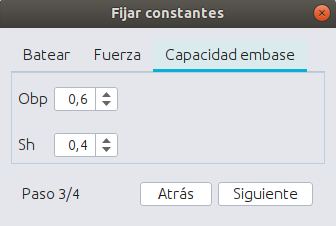
\includegraphics[width=0.45\textwidth]{figuras/fijarConstantes3.png}}
	
	\caption{Configuración de las constantes durante el proceso de importación} \label{fig:conf-constantes}
\end{figure}

Tomando como ejemplo los datos provenientes del fichero de béisbol, mostrados en la Figura \ref{fig:fichero-beisbol} y las constantes que se observan en la Figura \ref{fig:conf-constantes}, se obtienen como resultado los datos mostrados en la Figura \ref{fig:import-comp-tec}. Los datos resultantes y la información mostrada en las Tablas \ref{transf-pel}, \ref{pref-rol-of-pel} y \ref{pref-rol-def-pel} son calculados con las mismas constantes. A simple vista se pueden observar que son iguales. Se puede llegar a la conclusión entonces, que el proceso de importación funciona correctamente. 

\begin{figure} [H]
	\centering
	\subfigure[Experiencia de los jugadores]{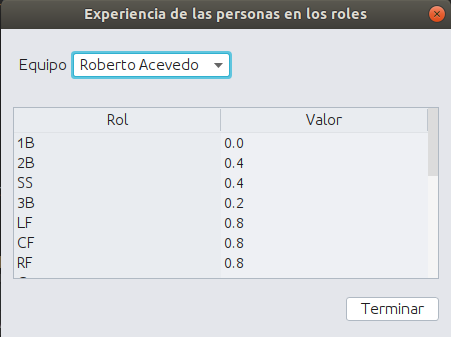
\includegraphics[width=0.6\textwidth]{figuras/importarExpEval.png}}
	\subfigure[Competencias técnicas de los jugadores]{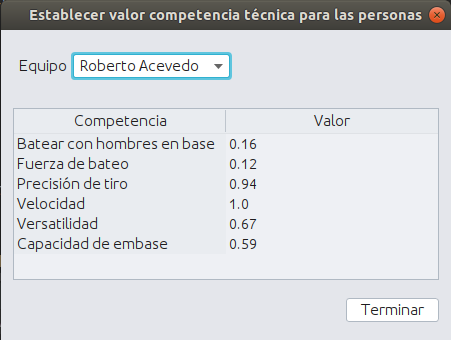
\includegraphics[width=0.6\textwidth]{figuras/importarCompTecEval.png}}
	
	\caption{Resultado de la importación para el problema de béisbol} \label{fig:import-comp-tec}
\end{figure}

\subsection{Exportación de los datos}

El proceso de exportación de los datos consta de cuatro grandes pasos (ver Figura \ref{fig:proceso-export}). El usuario que responde al rol importador es el encargado de cada uno de ellos. El primer paso es donde se eligen los equipos a solucionar (ver Figura \ref{fig:equipos-exportar}). El siguiente se encarga de elegir las personas de interés para formar parte de los equipos seleccionados (ver Figura \ref{fig:personas-exportar}).

\begin{figure}[H]
	\centering
	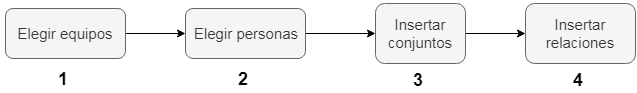
\includegraphics[width=1\textwidth]{figuras/flujoExport.png}
	\caption{Proceso de exportación de los datos}\label{fig:proceso-export}
\end{figure} 

\begin{figure}[H]
	\centering
	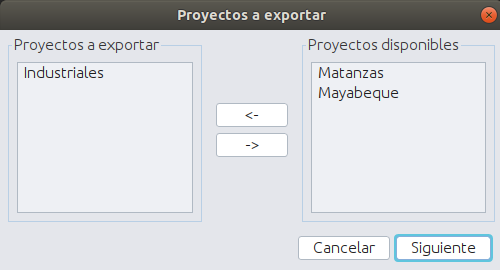
\includegraphics[width=0.6\textwidth]{figuras/exportarEquipo.png}
	\caption{Ventana para elegir los equipos a exportar}\label{fig:equipos-exportar}
\end{figure}   

\begin{figure}[H]
	\centering
	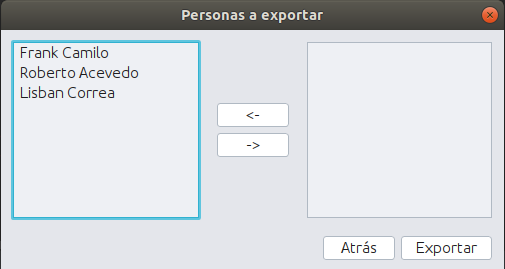
\includegraphics[width=0.6\textwidth]{figuras/exportarPersonas.png}
	\caption{Ventana para elegir las personas a exportar}\label{fig:personas-exportar}
\end{figure}   

Después que fuesen elegidos los equipos y las personas, se insertan todos los conjuntos que se relacionan con ellos, y a su vez, las relaciones que existen entre esos conjuntos. Este proceso se realiza de esta forma debido a la dependencia existente los datos.
 
\subsubsection{Descripción de las tablas de TEAMSOFT$^+$}
Como parte de este trabajo se desarrolla un sistema que permite la transformación de datos que almacenan información de las personas y se encuentran en ficheros externos, en datos entendibles por el sistema TEAMSOFT$^+$. Los valores de competencia y preferencia de las personas asignados a estas, resultan objetivo, partiendo que se obtienen de datos almacenados en sistemas, sitios o herramientas que constituyen la fuente de datos en cada uno de los problemas analizados en este trabajo. Una vez importada la información de las personas y realizadas las transformaciones pertinentes en cada caso, es necesario exportar la información hacia la base de datos con la que trabaja el sistema TEAMSOFT$^+$ para su solución posterior. En la Figura \ref{fig:tablas-teamsoft} se muestran todas las tablas de la base de datos utilizadas en la exportación por la herramienta desarrollada como parte de este trabajo. Marcadas en un rectángulo rojo, están aquellas en las que se realiza inserción de datos. A continuación se realiza una breve explicación de cada una de ellas:

\begin{description}
	\item[competence:] tabla donde se guardan todas las competencias, ya sean técnicas o genéricas. 
	
	\item[competence\_dimension:] esta tabla almacena una descripción para cada competencia, además de registrar el nivel en que se necesita.
	
	\item[competence\_importance:] tabla que almacena la importancia de cada competencia.
	
	\item[competence\_value:] almacena para cada persona, el nivel que posee en cada competencia.
	
	\item[conflict\_index:] tabla donde se registra el índice de conflicto entre las personas.
	
	\item[cycle:] almacena la estructura, fecha inicio y fecha fin de cada proyecto.
	
	\item[incompatible\_roles:]  guarda los roles incompatibles en todos los proyectos.
	
	\item[levels:] tabla donde se configura los niveles que tienen las competencias. 
	
	\item[person\_group:] almacena los grupos a los que pertenecen las personas. Existe una jerarquía de grupos, donde un grupo puede ser padre de otro, y por tanto, hereda sus personas.
	
	\item[personal\_interest:] almacena las preferencias de las personas por los roles.
	
	\item[project:] tabla donde se guardan todos los proyectos.
	
	\item[project\_role\_incomp:] registra todos los roles incompatibles por proyecto.
	
	\item[project\_roles:] tabla que almacena los roles necesarios en cada proyecto, así como la carga y el número de personas necesarias para desempeñarlos. 
	
	\item[project\_structure:] se registra la estructura de los proyectos.
	
	\item[project\_tech\_competence:] en cada proyecto, para cada rol, se registran las 
	competencias técnicas necesarias, así como el nivel en que se necesitan y la importancia que posee. 
	
	\item[role:] se almacenan todos los roles.
	
	\item[role\_competition:] para cada rol, se almacena la importancia y nivel en que se necesitan las competencias genéricas.
	
	\item[role\_experience:] experiencia de los trabajadores en los roles
	
	\item[role\_load:] carga qu representa ocupar un rol. Esta tabla no es utilizada por el problema de la pelota debido a que no influye el tiempo.
	
	\item[work:] tabla donde se almacenan las personas.
	
	\item[work\_conflict:] se registran las incompatibilidades entre las personas.
\end{description}

\begin{figure}[H]
	\centering
	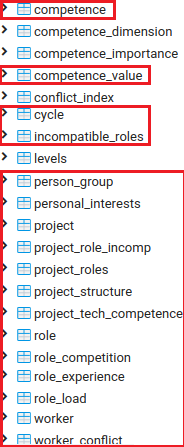
\includegraphics[width=0.23\textwidth]{figuras/tablasTeamSoft.png}
	\caption{Tablas utilizadas de la base de datos de TEAMSOFT$^+$}\label{fig:tablas-teamsoft}
\end{figure}

\subsubsection{Mapeo de los datos}
Para validar el correcto funcionamiento de la herramienta, resulta necesario conocer qué información de la gestionada, es necesario exportar a TEAMSOFT$^+$, y en qué tabla de la base de datos de este, se almacena. En caso de no existir un mapeo directo entre ambas bases de datos,  debe realizarse una transformación.\\

Como parte del tercer paso de la Figura \ref{fig:proceso-export} se procede a la inserción de los conjuntos en la base de datos de TEAMSOFT$^+$. Como primer paso dentro de este, se insertan todos los equipos elegidos en la tabla \textbf{project}. TEAMSOFT$^+$ organiza a las personas a través de grupos. A la hora de exportar las personas hacia TEAMSOFT$^+$, es necesario que siga este formato. Para lograr esto se crea un nuevo grupo en la tabla \textbf{person\_group}, y todas las personas elegidas se insertan en la tabla \textbf{worker} asociadas al nuevo grupo. Después se procede a la inserción de los roles pertenecientes a los proyectos seleccionados en la tabla \textbf{role}. Quedando este proceso como se observa en la Figura \ref{fig:insert-equipo-y-personas}.

\begin{figure}[H]
	\centering
	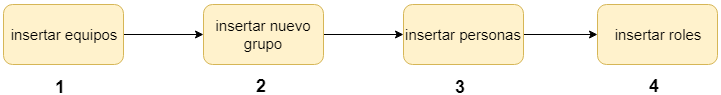
\includegraphics[width=0.8\textwidth]{figuras/insertEquipoPersonas.png}
	\caption{Insertar equipos y personas}\label{fig:insert-equipo-y-personas}
\end{figure}

El diseño de la base de datos implementado en la herramienta, mantiene por separado las competencias técnicas de las genéricas. Mientras que en la base de datos de TEAMSOFT$^+$ se gestionan en una sola tabla. Se garantiza la distinción entre ellas, utilizando el campo booleano \textit{technical}. Cuando se realiza la exportación, todas las competencias, tanto técnicas como genéricas, se insertan en la tabla \text{competence}. Para el caso de las competencias técnicas, el valor del campo booleano sería verdadero, y falso para las genéricas.

Una vez finalizado el tercer paso de la Figura \ref{fig:proceso-export}, se procede insertar todos los datos de las relaciones existentes entre los conjuntos exportados. Primeramente, se insertan todos los roles pertenecientes a los equipos en la tabla \textbf{project\_role}. Para esto es necesario realizar un cambio. En la herramienta la carga de trabajo se gestiona en una escala de cero a uno, mientras que en la base de datos de TEAMSOFT$^+$ se maneja en una escala del uno al cuatro (tabla \textbf{role\_load}). Para lograr la transformación, se separa la escala del cero al uno en cuatro conjuntos de igual tamaño, en función de dónde le corresponda el valor, es la escala que toma en la base de datos de TEAMSOFT$^+$. Por ejemplo, si la carga del rol $r_1$ en el equipo $e_1$ fuese de 0.34, su valor, una vez transformado le corresponde 3 (Media). La Tabla \ref{table:transformacion-carga} refleja estas transformaciones.

\begin{table}[H]
	\centering
	\caption{Transformación de los valores de la carga de los roles}\label{table:transformacion-carga}
	\begin{tabular}{c | c | c}
		\toprule[1.7pt]
		Valores de la Herramienta & Valores TEAMSOFT$^+$ & Descripción               \\ \midrule
		        0.0 - 0.25          & 4                    & Baja                      \\ 
		        0.26 - 0.50         & 3                    & Media                     \\ 
		        0.51 - 0.75         & 2                    & Alta                      \\ 
		        0.76 - 1.0          & 1                    & Muy alta \\ \bottomrule[1.1pt]
	\end{tabular}
\end{table}

Una vez insertado los roles a los equipos, se inserta entonces, las incompatibilidades entre los roles en los equipos. Esto se realiza en la tabla \textbf{project\_role\_incom}. El siguiente paso sería entonces, insertar el valor que se necesita para cada competencia técnica en los roles de los proyectos en la tabla \textbf{project\_tech\_competence}. En este paso hay que realizar algunas transformaciones. Esta tabla gestiona la importancia para cada competencia, además del nivel que se necesita en ese rol para poder desempeñarlas. Al no gestionarse la importancia de las competencias en la herramienta, se mantiene fijo el valor en el nivel más bajo (alguna medida). El nivel necesario de las competencias se expresa en una escala del uno al cuatro, mientras que en la herramienta se gestiona de cero a uno. En la Tabla \ref{table:transformacion-nivel-competencia} se realiza el proceso de conversión.

\begin{table}[H]
	\centering
	\caption{Transformación de los niveles de las competencias}\label{table:transformacion-nivel-competencia}
	\begin{tabular}{c | c | c}
		\toprule[1.7pt]
		Valores de la Herramienta & Valores TEAMSOFT$^+$ & Descripción               \\ \midrule
		0.0 - 0.25          & 1                    & en partida                      \\ 
		0.26 - 0.50         & 2                    & en desarrollo                     \\ 
		0.51 - 0.75         & 3                    & en avance               \\ 
		0.76 - 1.0          & 4                    & experto \\ \bottomrule[1pt]
	\end{tabular}
\end{table}

El siguiente paso sería insertar la relación entre las competencias genéricas y los roles en la tabla \textbf{role\_competition}. En esta tabla ocurre algo parecido a lo sucedido a la hora de exportar los datos de la tabla \textbf{project\_tech\_competence}, lo que esta vez no intervienen los equipos, solamente las competencias genéricas y los roles. La transformación sería la misma que se hizo en la Tabla \ref{table:transformacion-nivel-competencia}. También es necesario insertar las incompatibilidades entre los roles. Estas incompatibilidades son a nivel global, lo que significa en todos los equipos están presentes. Por ejemplo. El rol $r_1$ y el rol $r_2$ se definen como incompatibles en la tabla \textbf{incompatible\_roles}, estos roles serían incompatibles a su vez en todos los equipos.\\

Lo siguiente sería insertar las relaciones donde intervienen las personas. La primera relación a insertar sería, las incompatibilidades entre la personas en la tabla \textbf{worker\_conflict}. Una vez realizada esta operación se procede a insertar las preferencias de las personas por los roles y la experiencia de las personas en los roles en las tablas \textbf{personal\_interest} y \textbf{role\_experience}, respectivamente. La herramienta desarrollada permite la obtención de la experiencia de las personas por los roles, teniendo en cuenta tiempo que llevan ejerciéndolos y el tiempo total de experiencia. En el caso de las preferencias de las personas por los roles, en la base de datos de TEAMSOFT$^+$ se gestiona como un valor booleano, si lo prefiere o no. Mientras que en la herramienta se trata en valores en la escala de cero a uno. El autor decide entonces, realizar un punto de corte en la escala. Todo valor que esté por encima de 0.5 se considera como si la persona tuviese preferencia por el rol. El proceso de exportación de los datos culmina con la inserción el valor de las personas en las competencias en la tabla \textbf{competence\_value}. Como ya se mencionaba anteriormente, en la herramienta se tratan por separado las competencias técnicas y genéricas. También se mencionó con anterioridad que los valores que le otorga la herramienta a las competencias oscila en la escala de cero a uno. Por lo tanto las transformaciones son las mismas que las presentadas en la Tabla \ref{table:transformacion-nivel-competencia}. La Figura \ref{fig:flujo-completo} muestra el diagrama de flujo que explica todo el proceso.

\begin{figure}[H]
	\centering
	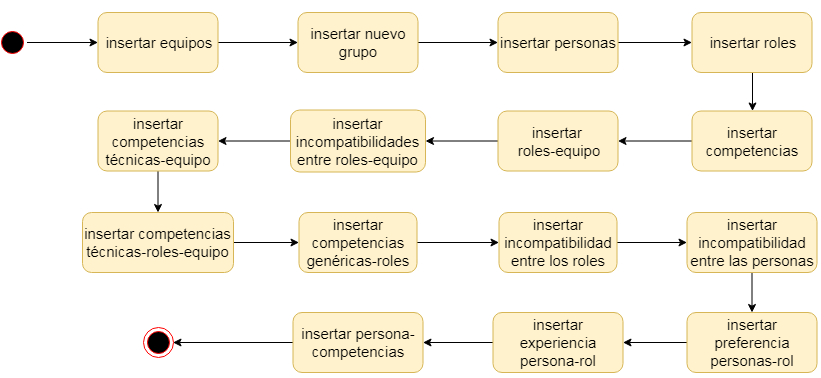
\includegraphics[width=0.9\textwidth]{figuras/flujoCompletoExport.png}
	\caption{Diagrama de flujo del proceso de exportación}\label{fig:flujo-completo}
\end{figure}

Se comprueba el correcto funcionamiento del proceso de exportación si TEAMSOFT$^+$ carga exitosamente los datos exportados por la herramienta. En las Figuras \ref{fig:exportar-competencias}, \ref{fig:exportar-roles} y \ref{fig:exportar-personas} se muestran algunas capturas de pantalla de TEAMSOFT$^+$, una vez culminado el proceso de exportación.

\begin{figure}[H]
	\centering
	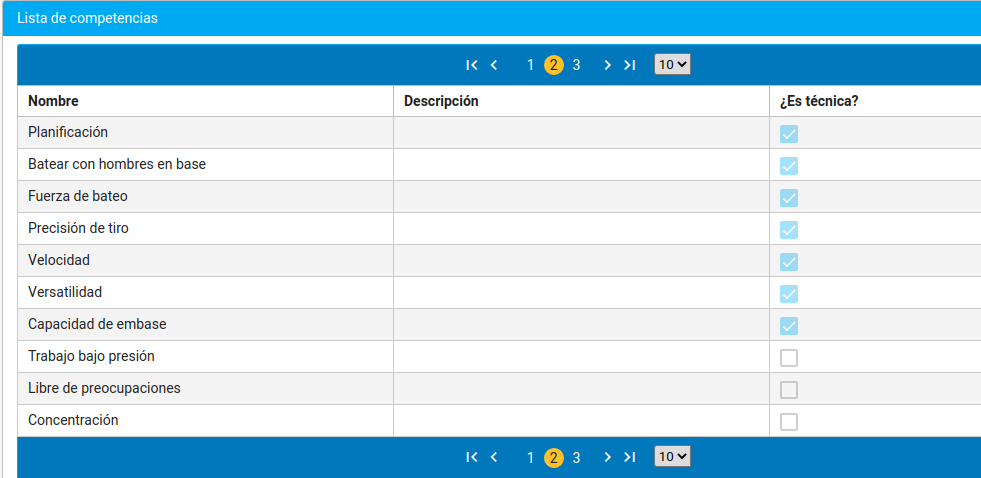
\includegraphics[width=0.9\textwidth]{figuras/exportarCompetencias.png}
	\caption{Ventana para gestionar las competencias en TEAMSOFT$^+$}\label{fig:exportar-competencias}
\end{figure}

\begin{figure}[H]
	\centering
	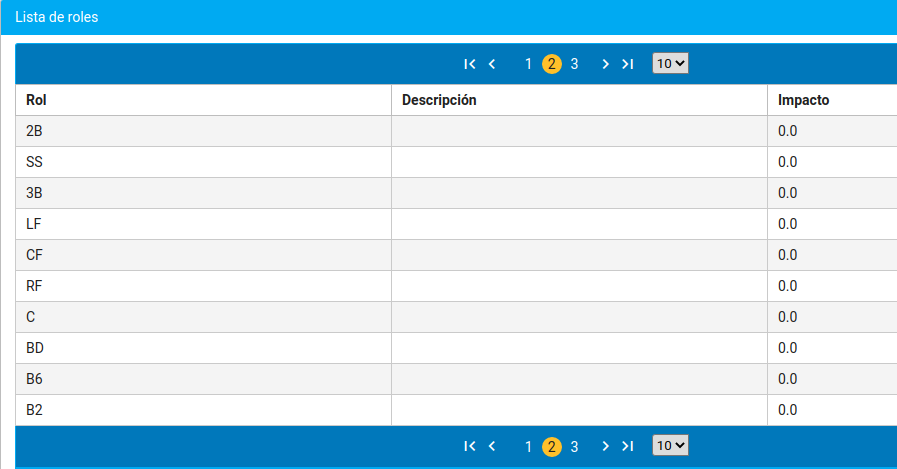
\includegraphics[width=0.9\textwidth]{figuras/exportarRoles.png}
	\caption{Ventana para gestionar los roles en TEAMSOFT$^+$}\label{fig:exportar-roles}
\end{figure}

\begin{figure}[H]
	\centering
	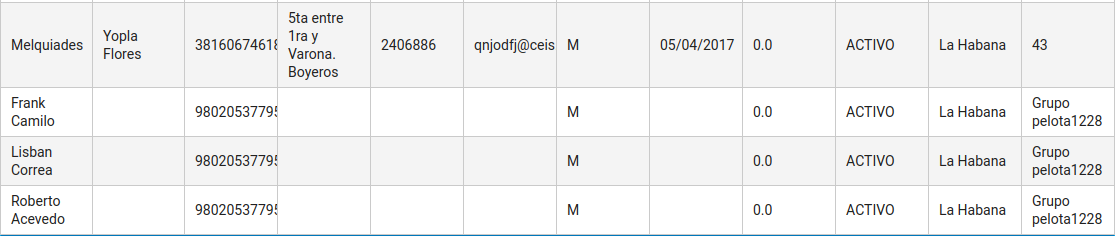
\includegraphics[width=1\textwidth]{figuras/exportarPersonasTeamsoft.png}
	\caption{Ventana para gestionar las personas en TEAMSOFT$^+$}\label{fig:exportar-personas}
\end{figure}

\section{Conclusiones parciales}
Con la terminación de este capítulo se llega a las siguientes conclusiones:
\begin{enumerate}
	\item Se implementó una herramienta para la obtención de las características de las personas para los problemas de conformación de equipos docentes y de béisbol, a partir de datos almacenados en sistemas, sitios o herramientas que constituyen la fuente de datos en cada uno de los problemas analizados en este trabajo.
	\item Se validó que los datos exportados por la herramienta son leídos satisfactoriamente por TEAMSOFT$^+$.
\end{enumerate}

	\chapter*{Conclusiones}
%Al finalizar este trabajo podemos afirmar que se cumplieron los objetivos trazados al inicio del mismo y se arribaron a las siguientes conclusiones:
Al finalizar este trabajo se arriban a las siguientes conclusiones:
\begin{enumerate}
	\item A través del análisis del estado del arte sobre la conformación de equipos se identificó que los modelos relacionados con los temas de béisbol y docencia no tienen en cuenta factores que contribuyan a la asignación de las personas a los roles del equipo. Por ejemplo las competencias necesarias para cumplir los roles, las preferencias de las personas por los roles, las incompatibilidades entre las personas, entre otros.
	\item Se identificaron los factores a tener en cuenta en la formación de equipos docentes y de béisbol.
	\item Se comprobó que es posible adaptar el modelo existente soportado en TEAMSOFT$^+$ a los problemas de béisbol y docencia.
	\item Se implementó una herramienta para la obtención de las características de los personas, a partir de las fuentes de datos correspondientes a estos problemas (sito oficial del béisbol cubano y sistema Pandora).
	\item Se validó que los datos exportados por la herramienta de sus fuentes de datos fueron almacenados correctamente en TEAMSOFT$^+$.
\end{enumerate}
	\chapter*{Recomendaciones}
Con vistas a darle continuidad a este trabajo se recomienda: 
\begin{enumerate}
	\item Realizar nuevamente los experimentos para el caso del problema de la docencia una vez implementada la funcionalidad de las preferencias de las personas por los equipos.
	\item Valorar la posibilidad de extender el modelo a otros problemas.
	\item Incorporar al pícher como un rol tener en cuenta en el problema de la pelota.
	\item Flexibilizar el cálculo de las competencias, permitiendo al usuario elegir distintos tipos de métodos.
\end{enumerate}
	\addcontentsline{toc}{chapter}{Conclusiones}
	\addcontentsline{toc}{chapter}{Recomendaciones}
	\addcontentsline{toc}{chapter}{Referencias bibliográficas}
	
	\bibliography{bib_tesis}
	\bibliographystyle{IEEEtran}
	
	\addcontentsline{toc}{chapter}{Anexo}
	\appendix
\clearpage{\renewcommand{\appendixname}{Anexos}

%===============================DOCENCIA==============================================

\chapter{Ejemplo de fichero para la importación de datos}
\begin{figure}[H]
	\centering
	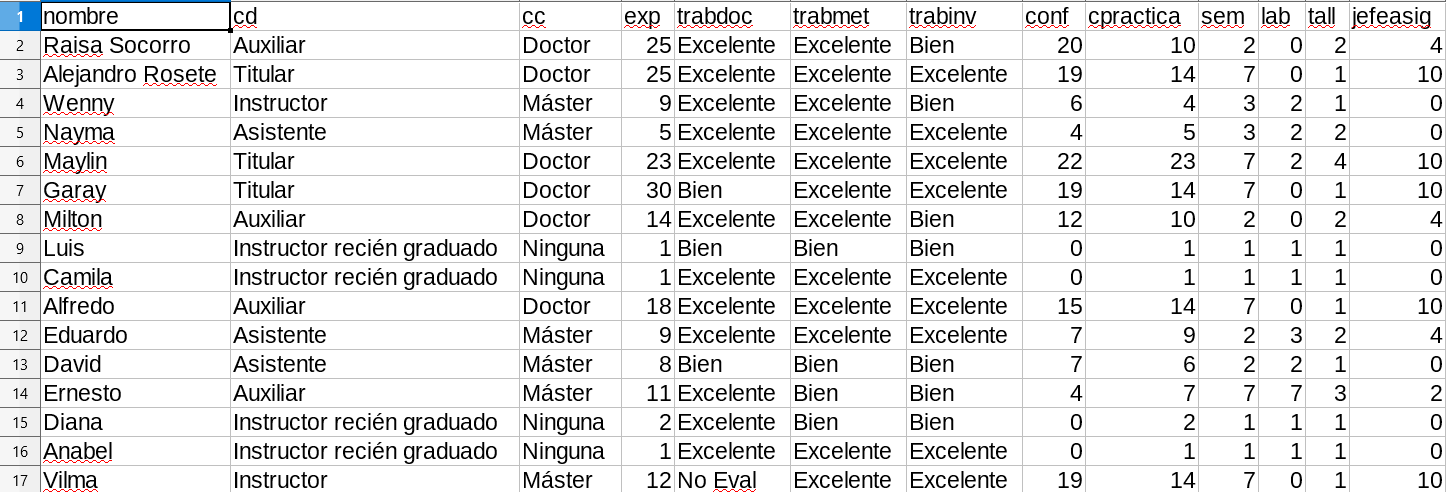
\includegraphics[width=.8\textwidth]{figuras/fichero-docencia.png}
	\caption{Fichero a importar para el contexto Formación de equipos de profesores para impartir docencia} \label{fig:fichero-docencia}
\end{figure}

\begin{figure}[H]

	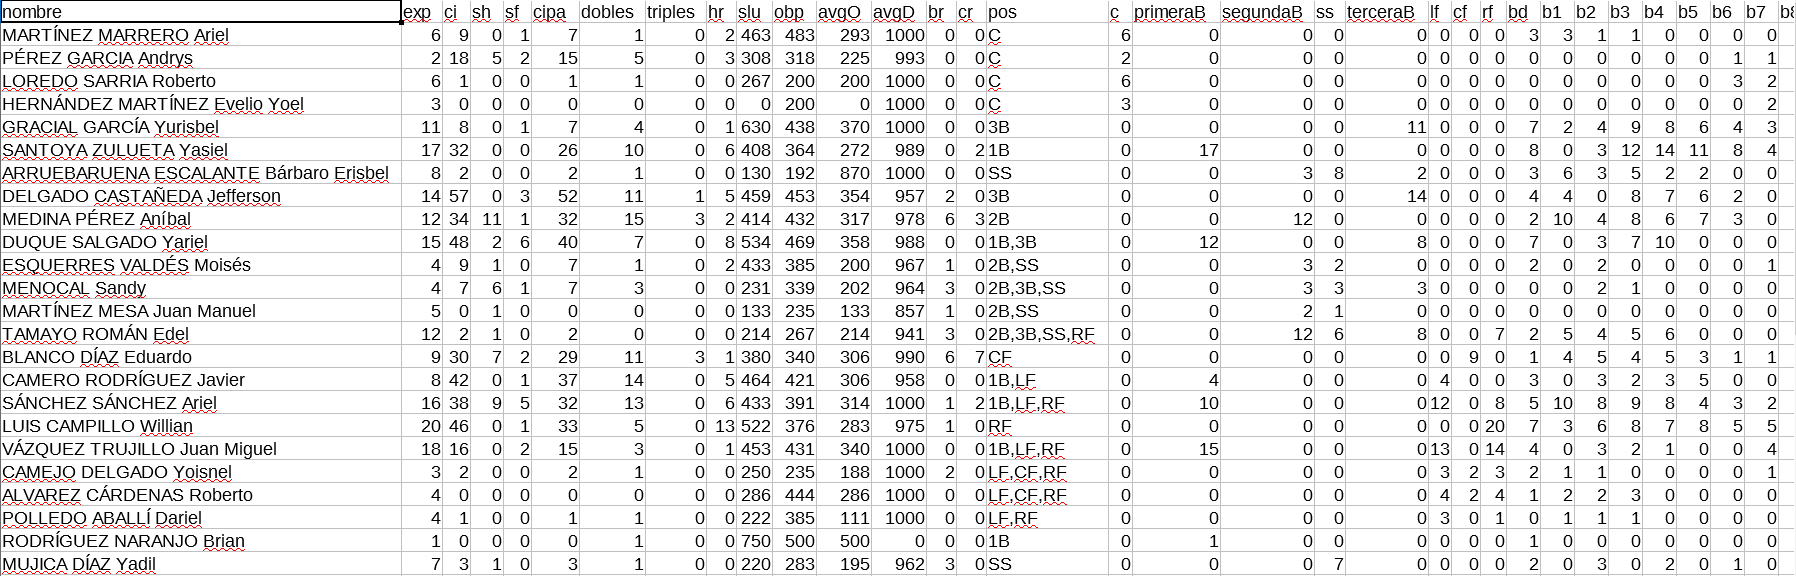
\includegraphics[width=\textwidth]{figuras/fichero-beisbol.png}
	\caption{Fichero a importar para el contexto Formación de un equipo de béisbol} \label{fig:fichero-beisbol}
\end{figure}



\chapter{Pantalla de seleccionar el fichero y establecer grupo}
\begin{figure}[H]
	\centering
	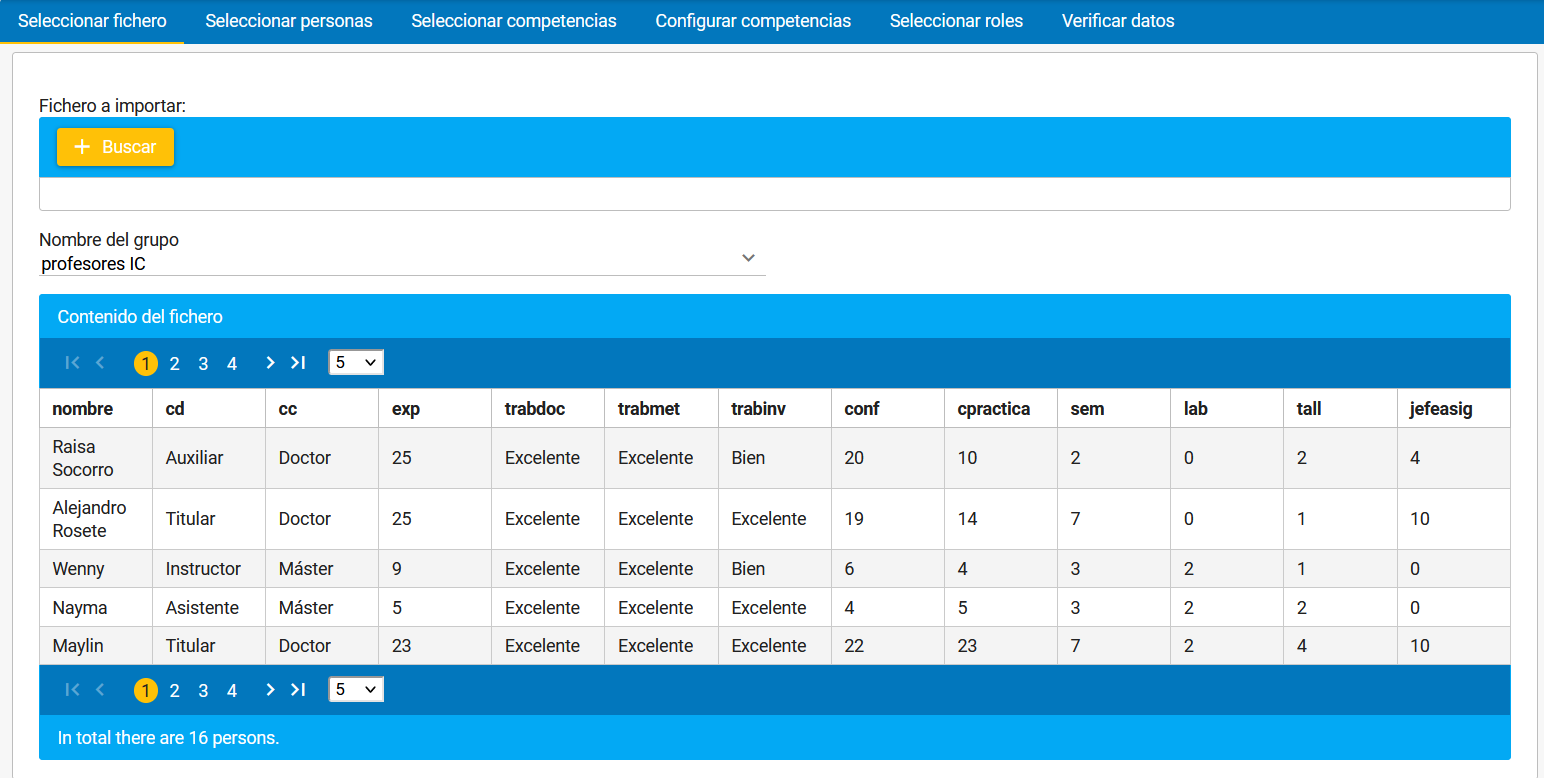
\includegraphics[width=\textwidth]{figuras/cargar_fichero_docencia.png}
	\caption{Pantalla cargar después de seleccionado el fichero y establecido el grupo (docencia)} \label{fig:cargar-fichero-docencia}
\end{figure}

\begin{figure}[H]
	\centering
	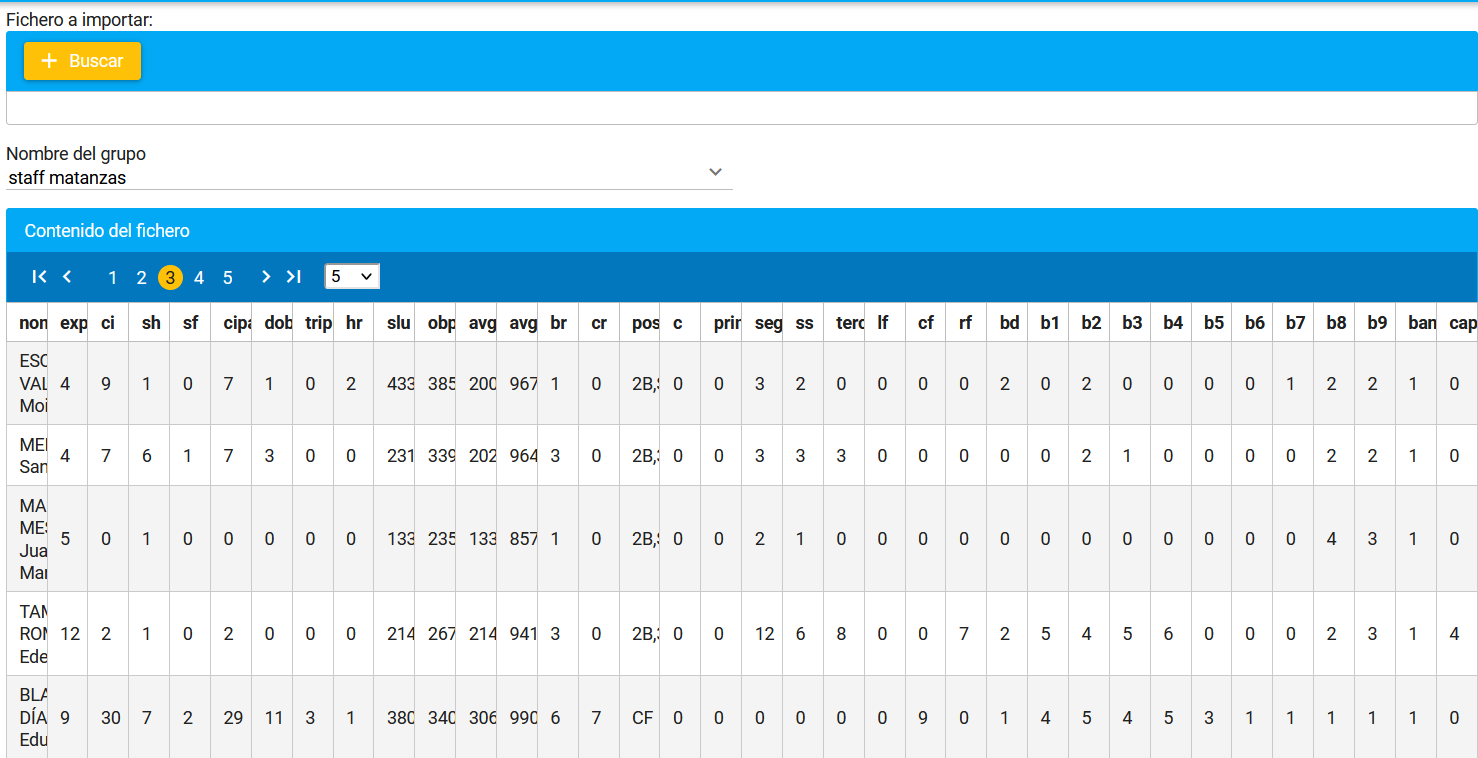
\includegraphics[width=\textwidth]{figuras/cargar_fichero_beisbol.png}
	\caption{Pantalla cargar después de seleccionado el fichero y establecido el grupo (béisbol)} \label{fig:cargar-fichero-beisbol}
\end{figure}


\chapter{Pantalla mapeo datos de las personas}
\begin{figure}[H]
	\centering
	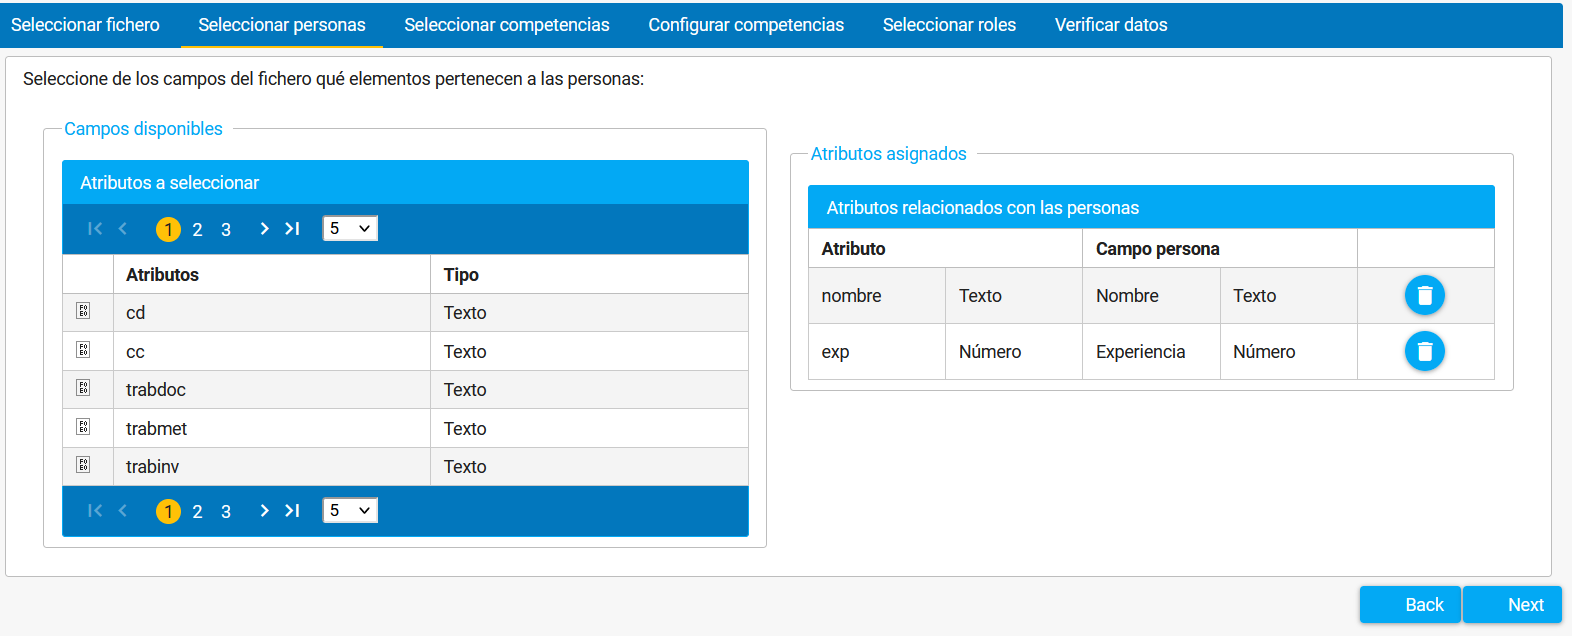
\includegraphics[width=\textwidth]{figuras/docencia_mapeo_atributos_personas.png}
	\caption{Asociar atributos del fichero a las personas (común para los dos problemas)} \label{fig:mapeo_atr_pers}
\end{figure}



%=======================Competencias=========================

%---------------------------DOCENCIA-----------------------------------------
\chapter{Pantalla configuración competencias}
\begin{figure}[H]
	\centering
	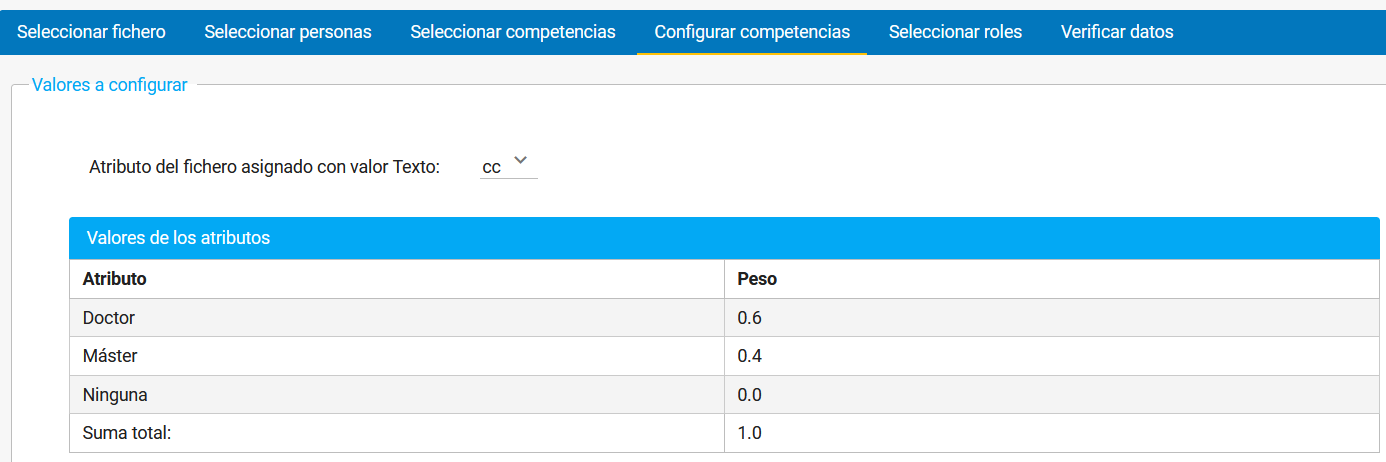
\includegraphics[width=\textwidth]{figuras/docencia_config_competencias_cc.png}
	\caption{Asociar peso a los valores del atributo cc (docencia)} \label{fig:conf_comp_cc_docencia}
\end{figure}

\begin{figure}[H]
	\centering
	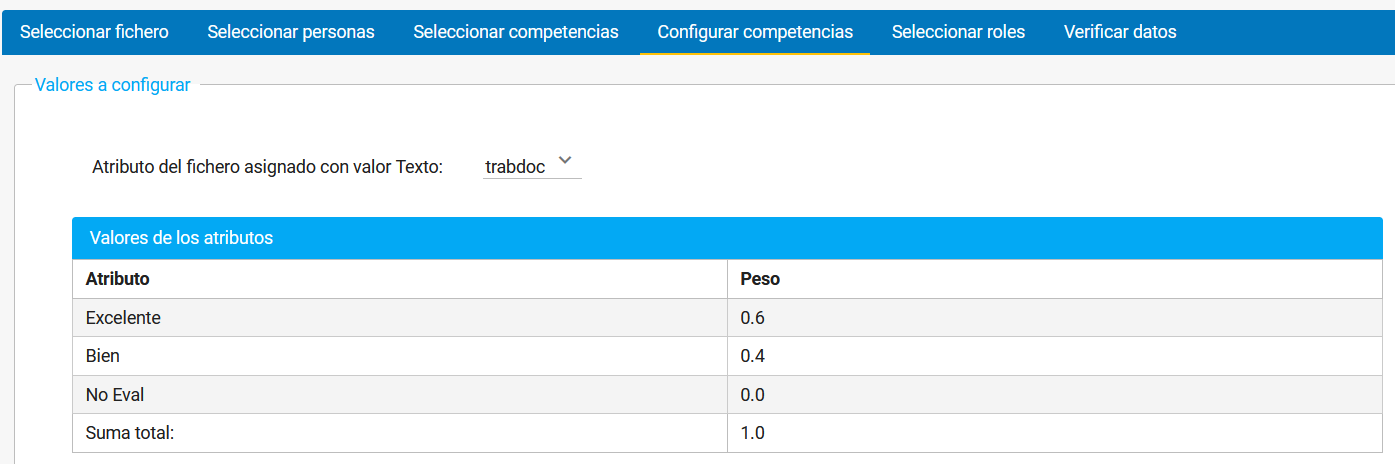
\includegraphics[width=\textwidth]{figuras/docencia_config_competencias_doc.png}
	\caption{Asociar peso a los valores del atributo trabdoc (docencia)} \label{fig:conf_comp_doc_docencia}
\end{figure}

\begin{figure}[H]
	\centering
	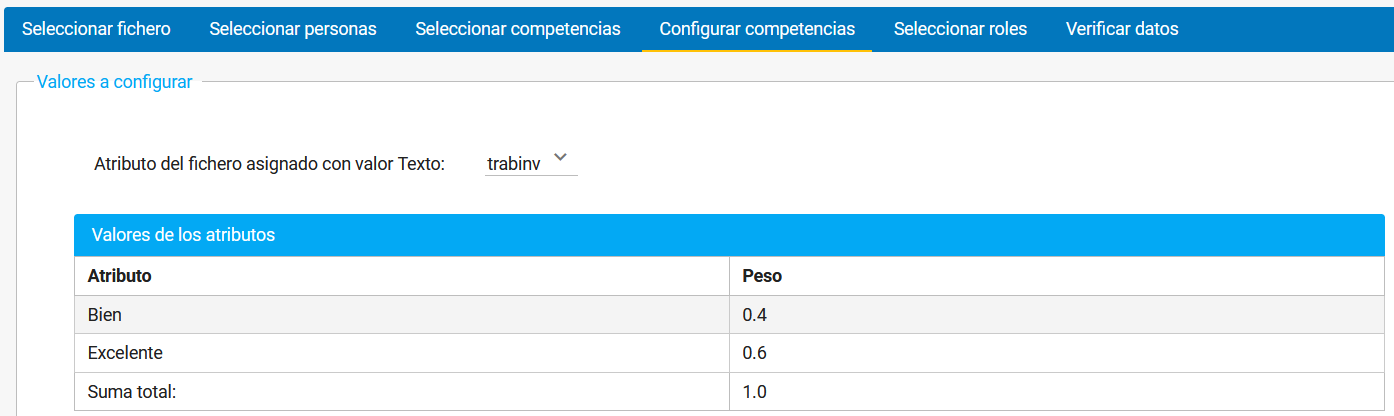
\includegraphics[width=\textwidth]{figuras/docencia_config_competencias_inv.png}
	\caption{Asociar peso a los valores del atributo trabinv (docencia)} \label{fig:conf_comp_inv_docencia}
\end{figure}

%----------------------------BEISBOL----------------------------------------

\begin{figure}[H]
	\centering
	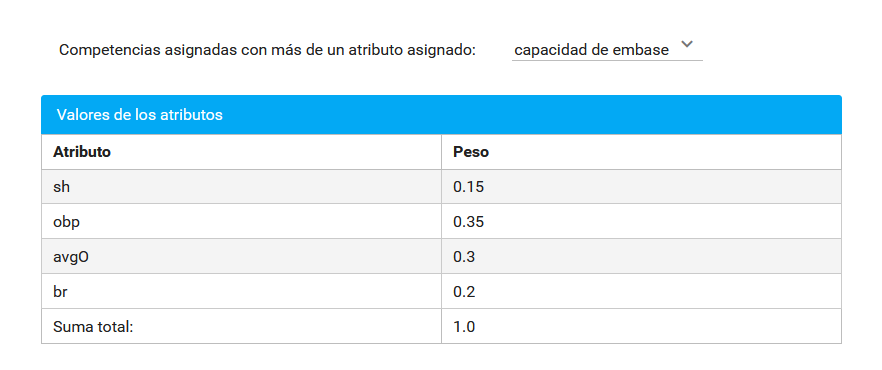
\includegraphics[width=\textwidth]{figuras/beisbol_conf_comp_ce.png}
	\caption{Asociar peso a los valores del atributo cc (béisbol)} \label{fig:conf_comp_ce_beisbol}
\end{figure}

\begin{figure}[H]
	\centering
	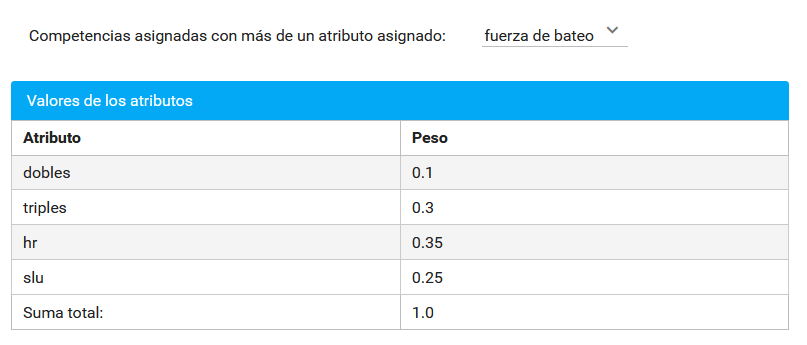
\includegraphics[width=\textwidth]{figuras/beisbol_conf_comp_fb.png}
	\caption{Asociar peso a los valores del atributo trabdoc (béisbol)} \label{fig:conf_comp_fb_beisbol}
\end{figure}

\begin{figure}[H]
	\centering
	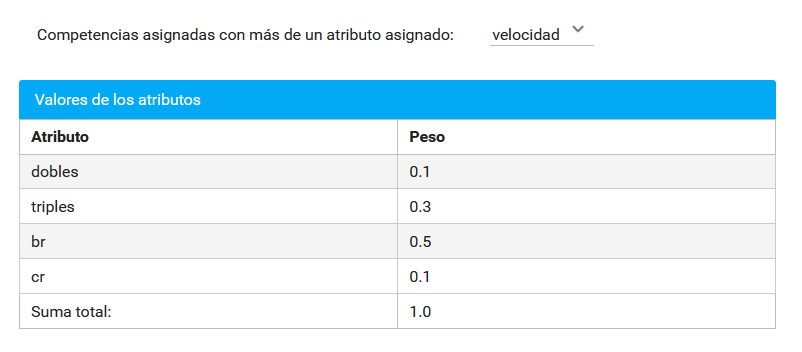
\includegraphics[width=\textwidth]{figuras/beisbol_conf_comp_v.png}
	\caption{Asociar peso a los valores del atributo trabinv (béisbol)} \label{fig:conf_comp_v_beisbol}
\end{figure}

%=======================Fin Competencias=========================

\chapter{Pantalla verificar datos}
\begin{figure}[H]
	\centering
	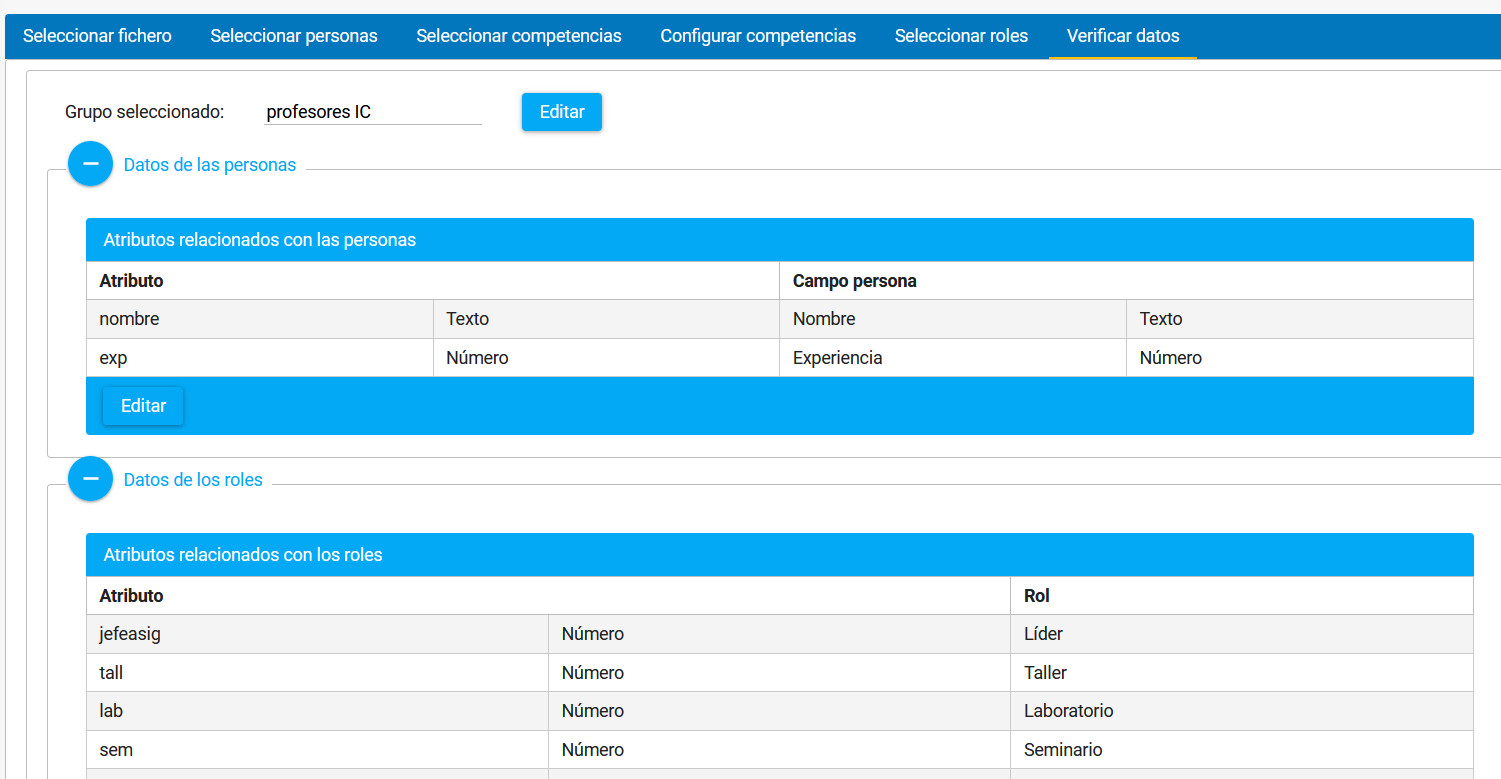
\includegraphics[width=\textwidth]{figuras/docencia_verificacion.png}
	\caption{Pantalla verificación de los datos (docencia)} \label{fig:verificar_datos_docencia}
\end{figure}

\begin{figure}[H]
	\centering
	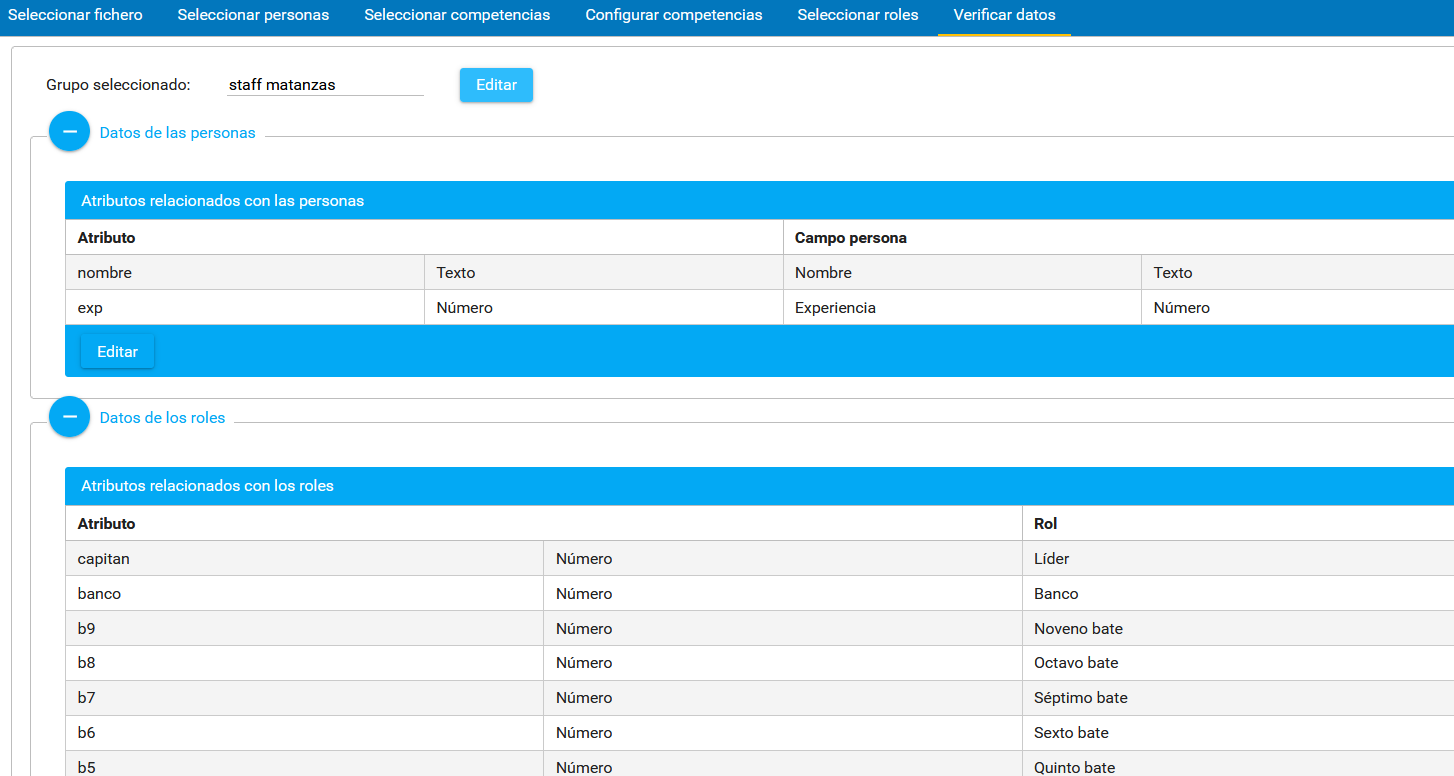
\includegraphics[width=\textwidth]{figuras/beisbol_verificacion.png}
	\caption{Pantalla verificación de los datos (béisbol)} \label{fig:verificar_datos_beisbol}
\end{figure}



\chapter{Pantalla mensaje información}
\begin{figure}[H]
	\centering
	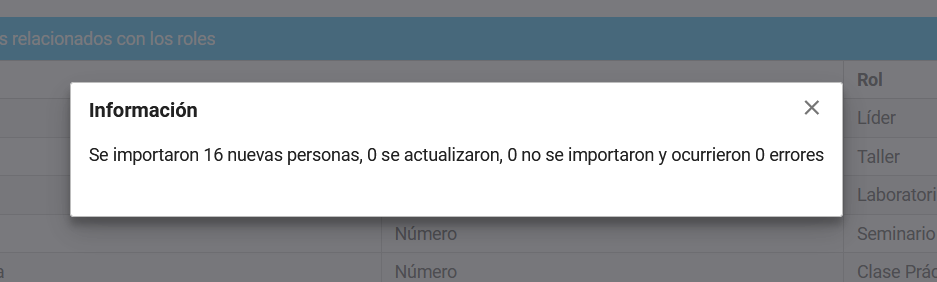
\includegraphics[width=\textwidth]{figuras/docencia_resultados.png}
	\caption{Mensaje de información después de importar (docencia)} \label{fig:resultados_docencia}
\end{figure}

\begin{figure}[H]
	\centering
	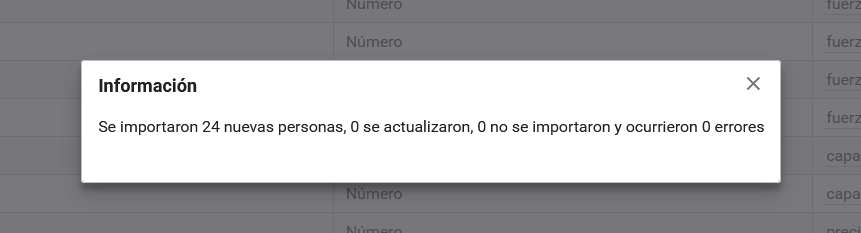
\includegraphics[width=\textwidth]{figuras/beisbol_resultados.png}
	\caption{Mensaje de información después de importar (béisbol)} \label{fig:resultados_beisbol}
\end{figure}



\chapter{Pantalla lista de personas importadas}
\begin{figure}[H]
	\centering
	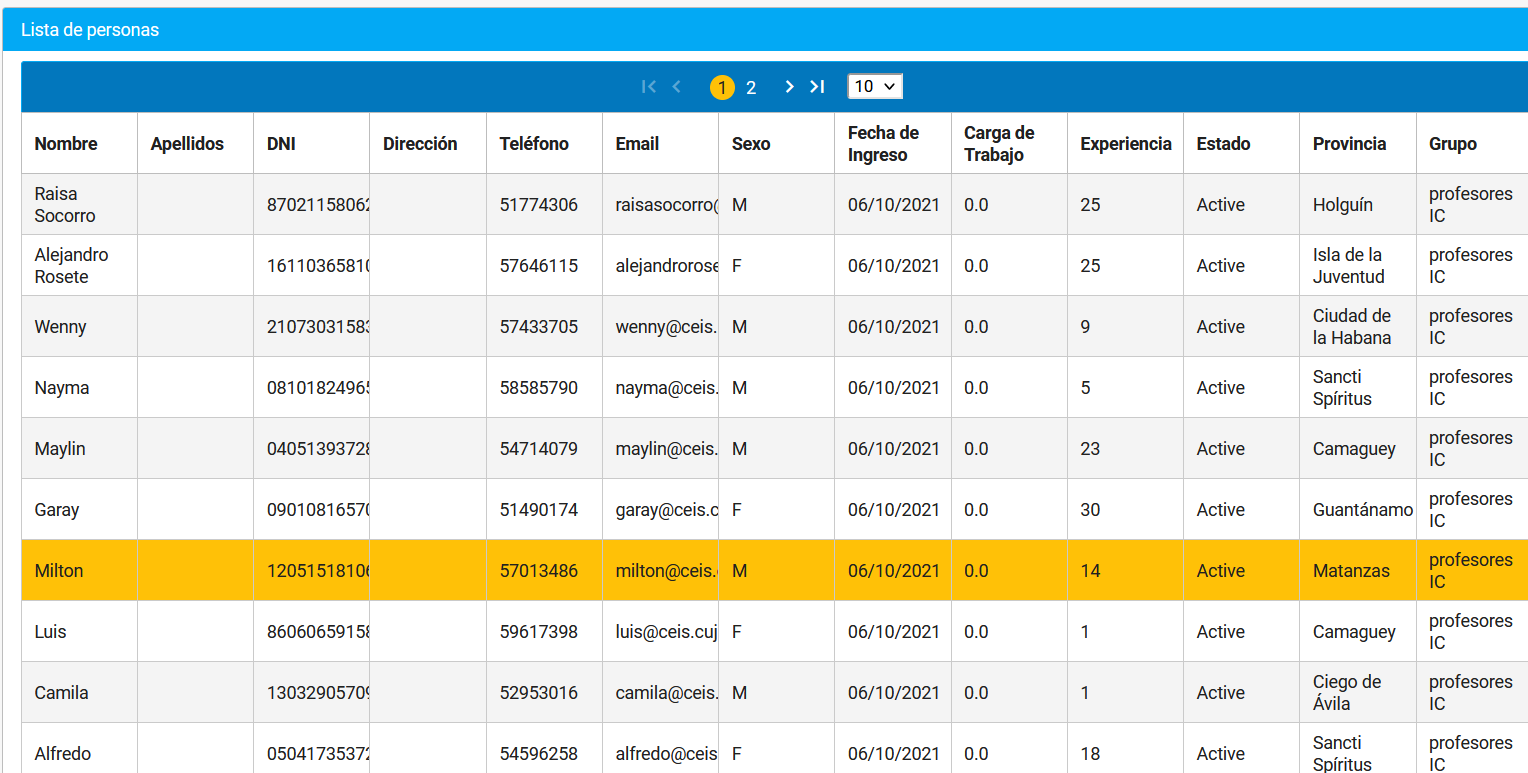
\includegraphics[width=\textwidth]{figuras/milton_seleccionado.png}
	\caption{Listado de personas importadas (docencia)} \label{fig:lista_profesores_docencia}
\end{figure}

\begin{figure}[H]
	\centering
	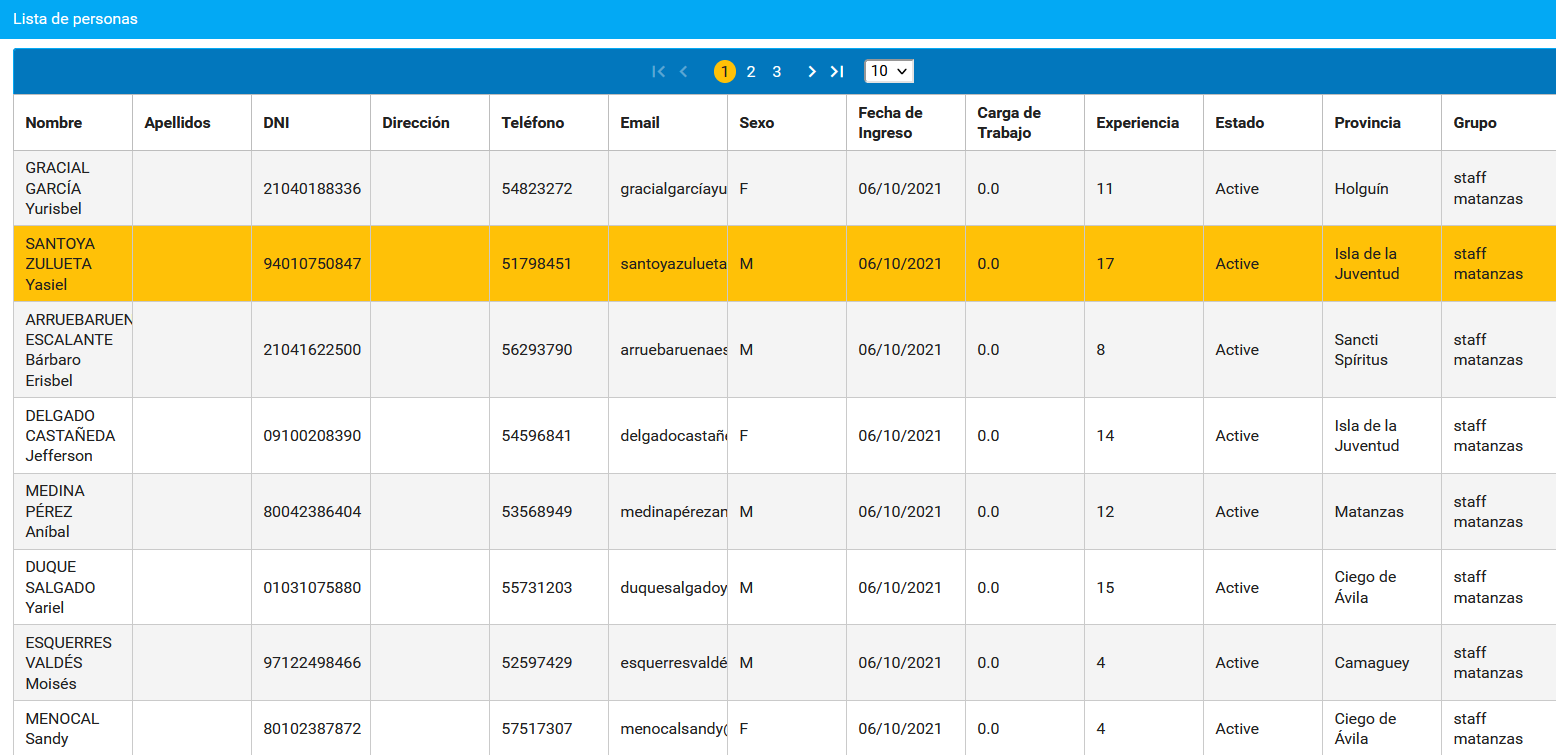
\includegraphics[width=\textwidth]{figuras/besibol_santoya_seleccionado.png}
	\caption{Listado de personas importadas (béisbol)} \label{fig:lista_jugadores_beisbol}
\end{figure}




\chapter{Pantalla competencias genéricas de una persona}
\begin{figure}[H]
	\centering
	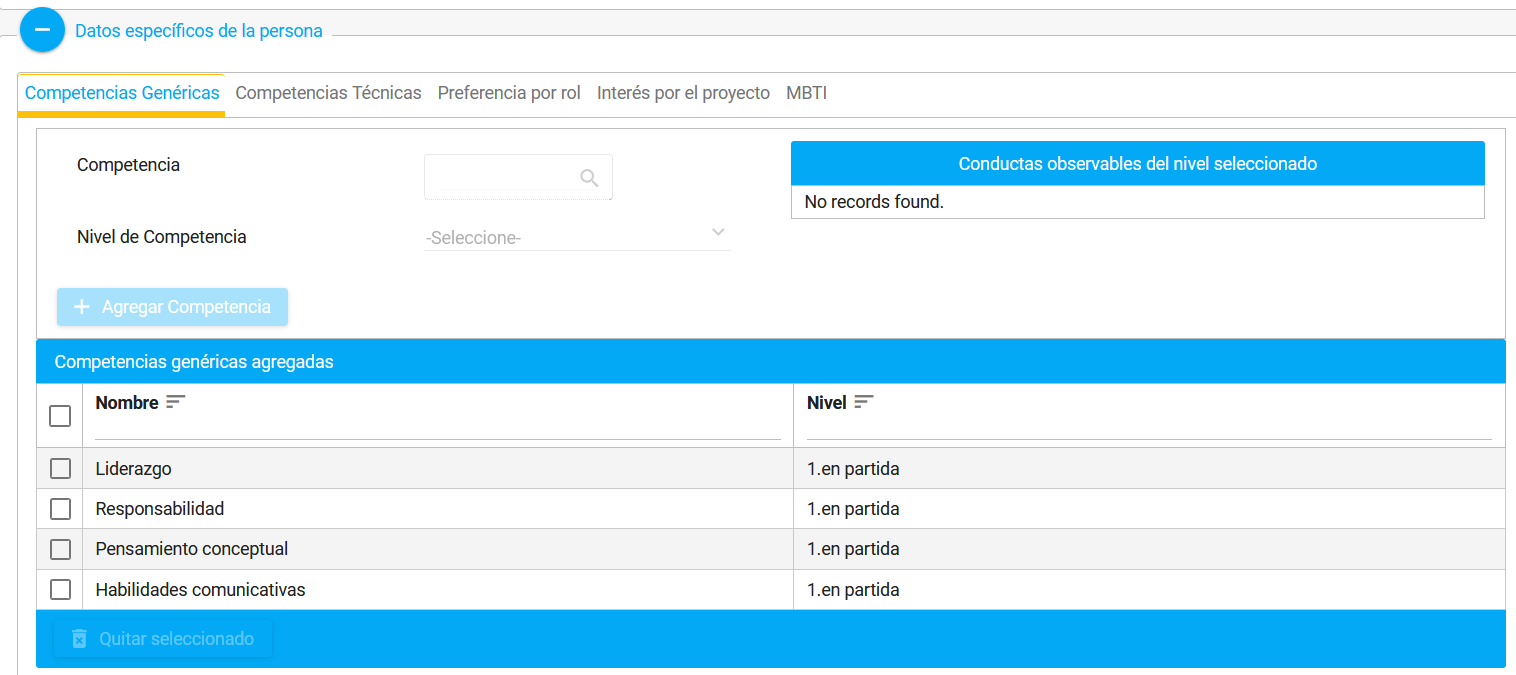
\includegraphics[width=\textwidth]{figuras/milton_comp_genericas.png}
	\caption{Competencias genéricas de Milton (docencia)} \label{fig:comp_genericas_docencia}
\end{figure}

\begin{figure}[H]
	\centering
	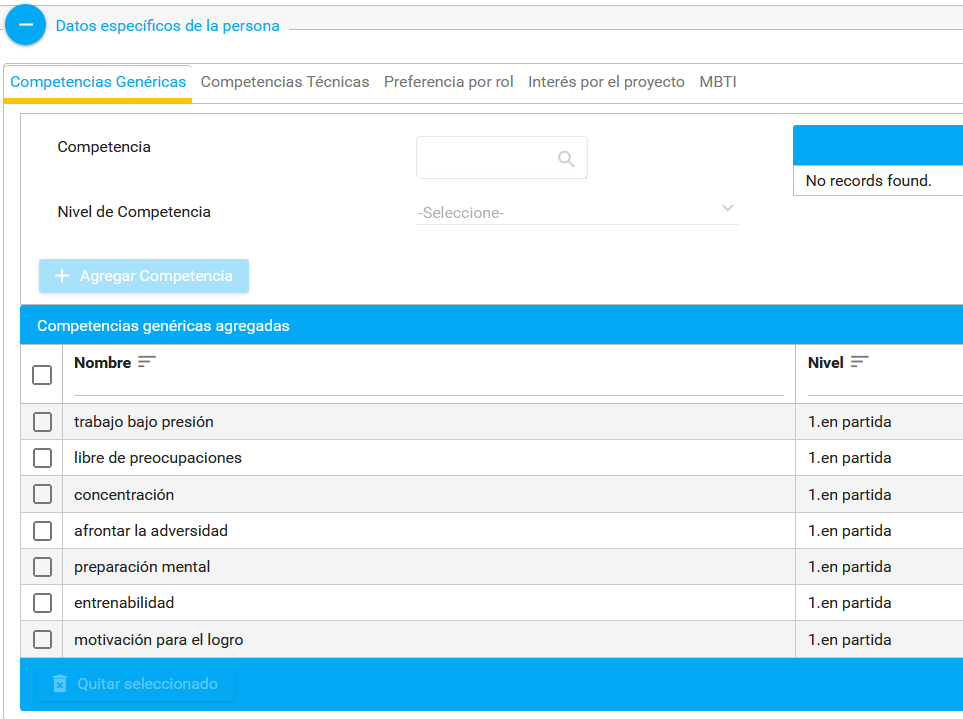
\includegraphics[width=\textwidth]{figuras/beisbol_santoya_compg.png}
	\caption{Competencias genéricas de Santoya (béisbol)} \label{fig:comp_genericas_beisbol}
\end{figure}


\chapter{Pantalla competencias técnicas de una persona}
\begin{figure}[H]
	\centering
	\includegraphics[width=\textwidth]{figuras/milton_competencias_tecnicas.png}
	\caption{Competencias técnicas de Milton (docencia)} \label{fig:comp_tecnicas_docencia}
\end{figure}

\begin{figure}[H]
	\centering
	\includegraphics[width=\textwidth]{figuras/milton_competencias_tecnicas.png}
	\caption{Competencias técnicas de Santoya (béisbol)} \label{fig:comp_tecnicas_beisbol}
\end{figure}

\chapter{Pantalla preferencia por los roles de una persona}
\begin{figure}[H]
	\centering
	\includegraphics[width=\textwidth]{figuras/milton_preferencia_roles.png}
	\caption{Preferencia de Milton por los roles (docencia)} \label{fig:pref_roles_docencia}
\end{figure}

\begin{figure}[H]
	\centering
	\includegraphics[width=\textwidth]{figuras/beisbol_santoya_roles.png}
	\caption{Preferencia de Santoya por los roles (béisbol)} \label{fig:pref_roles_beisbol}
\end{figure}

% configuración
\chapter{Pantalla de configuración de la importación}
\begin{figure}[H]
	\centering
	\includegraphics[width=\textwidth]{figuras/configuracion_importacion.png}
	\caption{Configuración de la importación} \label{fig:configuracion-problemas}
\end{figure}

\chapter{Configuración de las competencias requridas en los proyectos}

\begin{figure}[H]
	\centering
	\includegraphics[width=\textwidth]{figuras/conf-roles-comp-asignatura.png}
	\caption{Configuración de las competencias para todas las asignaturas} \label{fig:conf-roles-comp-asignatura}
\end{figure}

\begin{figure}[H]
	\centering
	\includegraphics[width=\textwidth]{figuras/beisbol_conf_comp_rol1.png}
	\caption{Configuración de las competencias en los roles 1ra parte (béisbol)} \label{fig:conf-roles-comp-pelota}
\end{figure}

\begin{figure}[H]
	\centering
	\includegraphics[width=\textwidth]{figuras/beisbol_conf_comp_rol2.png}
	\caption{Configuración de las competencias en los roles 2da parte (béisbol)} \label{fig:conf-roles-comp-pelota1}
\end{figure}

\begin{figure}[H]
	\centering
	\includegraphics[width=\textwidth]{figuras/beisbol_conf_comp_rol3.png}
	\caption{Configuración de las competencias en los roles 3ra parte (béisbol)} \label{fig:conf-roles-comp-pelota2}
\end{figure}


\chapter{Nivel de las personas en las competencias}

\begin{table}[H]
	\centering
	\hspace{2cm}
	\caption{Nivel de los profesores por competencias: Trabajo docente (TD), Trabajo metodológico (TM), Trabajo investigativo (TI), Categoría docente (CD) y Grado científico (GC)}\label{table:nivel-pers-comp2}
	%	\scalebox{.87}{
	\begin{tabular}{l l l l l l}
		\toprule
		\multirow{2}{2cm}{\textbf{Profesor}} &           \multicolumn{4}{c}{\textbf{Competencias}}           &  \\ \cline{2-6}
		                                       & \textbf{TD}   & \textbf{TM}   & \textbf{TI}   & \textbf{CD}   & \textbf{GC}   \\ \midrule
		Wenny                                  & Experto       & Experto       & En desarrollo & En desarrollo & En avance     \\ \hline
		Nayma                                  & Experto       & Experto       & Experto       & En avance     & En avance     \\ \hline
		Garay                                  & En avance     & Experto       & Experto       & Experto       & Experto       \\ \hline
		Milton                                 & Experto       & Experto       & En desarrollo & Experto       & Experto       \\ \hline
		Alfredo                                & Experto       & Experto       & Experto       & Experto       & Experto       \\ \hline
		Eduardo                                & Experto       & Experto       & Experto       & En avance     & En avance     \\ \hline
		David                                  & En avance     & En desarrollo & En desarrollo & En avance     & En avance     \\ \hline
		Ernesto                                & Experto       & En desarrollo & En desarrollo & Experto       & En avance     \\ \hline
		Diana                                  & Experto       & En desarrollo & En desarrollo & En partida    & En desarrollo \\ \hline
		Anabel                                 & Experto       & Experto       & Experto       & En partida    & En desarrollo \\ \hline
		Vilma                                  & En desarrollo & Experto       & Experto       & En desarrollo & En avance     \\ \bottomrule
	\end{tabular}
	%}
\end{table}

\begin{table}[H]
	\centering
	%	\hspace{-4cm}
	\caption{Nivel de los jugadores en las competencias: Batear con hombres en base (B), Fuerza de bateo (F), Precisión de tiro (P), Capacidad de embase (E) y Velocidad (V)}\label{table:nivel-jugadores-comp2}
	\scalebox{.97}{
		\begin{tabular}{ p{2.6cm} c c c c c }
			\toprule
			\multirow{2}{2.5cm}{\textbf{Jugador}} &                 \multicolumn{5}{c}{\textbf{Competencias}}                  \\ \cline{2-6}
			                                      & \textbf{B}    & \textbf{P} & \textbf{F}    & \textbf{V}    & \textbf{E}    \\ \midrule
			Ariel Martínez                        & En partida    & Experto    & En partida    & En partida    & En desarrollo \\ \hline
			Roberto Loredo                        & En partida    & Experto    & En partida    & En partida    & En partida    \\ \hline
			Aníbal Medina                         & En avance     & Experto    & En avance     & Experto       & Experto       \\ \hline
			Evelio Hernández                      & En partida    & Experto    & En partida    & En partida    & En partida    \\ \hline
			Moisés Esquerres                      & En partida    & Experto    & En partida    & En partida    & En desarrollo \\ \hline
			Sandy Menocal                         & En partida    & Experto    & En partida    & En desarrollo & En desarrollo \\ \hline
			Juan Manuel Mesa                      & En partida    & Experto    & En partida    & En partida    & En desarrollo \\ \hline
			Edel Tamayo                           & En partida    & Experto    & En partida    & En partida    & En desarrollo \\ \hline
			Willian Luis                          & En desarrollo & Experto    & En avance     & En partida    & En desarrollo \\ \hline
			Juan Miguel                           & En desarrollo & Experto    & En partida    & En partida    & En desarrollo \\ \hline
			Yoisnel Camejo                        & En partida    & Experto    & En partida    & En partida    & En desarrollo \\ \hline
			Roberto Álvarez                       & En partida    & Experto    & En partida    & En partida    & En desarrollo \\ \hline
			Dariel Polledo                        & En partida    & Experto    & En partida    & En partida    & En desarrollo \\ \hline
			Brian Rodríguez                       & En partida    & En partida & En desarrollo & En partida    & En avance     \\ \hline
			Yadil Mujica                          & En partida    & Experto    & En partida    & En desarrollo & En desarrollo \\ \hline
			Yariel Duque                          & Experto       & Experto    & En desarrollo & En partida    & En desarrollo \\ \hline
			Javier Camero                         & En desarrollo & Experto    & En desarrollo & En partida    & En desarrollo \\ \hline
			Erisbel Arruebaruena                  & En partida    & Experto    & En partida    & En partida    & En desarrollo \\ \hline
			Eduardo Blanco                        & En desarrollo & Experto    & En desarrollo & Experto       & En desarrollo \\ \bottomrule
		\end{tabular}
	}
\end{table}

%\begin{figure}[H]
%	\centering
%	\includegraphics[width=.9\textwidth]{figuras/importancia_competencias.png}
%	\caption{Niveles de importancia para las competencias en un rol} \label{fig:nivel-importancia}
%\end{figure}


\chapter{Preferencia de las personas por los roles}

\begin{table}[H]
	\centering
	%	\hspace{-2cm}
	\caption{Preferencia de las personas por los roles: Líder (L), Conferencia (C), Clase práctica (CP), Seminario (S), Laboratorio (LB) y Taller (T)}\label{table:pref-pers-roles-doc2}
	%	\scalebox{.87}{
	\begin{tabular}{l c c c c c c }
		\toprule
		\multirow{2}{2.5cm}{\textbf{Profesor}} &                      \multicolumn{6}{c}{\textbf{Roles}}                       \\ \cline{2-7}
		                                       & \textbf{L} & \textbf{C} & \textbf{CP} & \textbf{S} & \textbf{LB} & \textbf{T} \\ \midrule
		Ernesto                                &            &            & X           & X          & X           &  \\ \hline
		Vilma                                  &            & X          & X           &            &  \\ \hline
		Garay                                  &            & X          & X           &            &  \\ \hline
		Diana                                  &            &            &             &            &  \\ \hline
		Anabel                                 &            &            &             &            &  \\ \hline
		Nayma                                  &            & X          & X           & X          &  \\ \hline
		Milton                                 &            & X          & X           &            &  \\ \hline
		Alfredo                                & X          & X          & X           &            &  \\ \hline
		Eduardo                                & X          & X          & X           & X          &  \\ \hline
		David                                  &            &            & X           & X          &  \\ \hline
		Wenny                                  &            &            & X           & X          &             &  \\ \bottomrule
	\end{tabular}
	%}
\end{table}

\begin{table}[H]
	\centering
	%	\hspace{-4cm}
	\caption{Preferencia de los jugadores por los roles}\label{table:pref-pers-roles-pel2}
	%	\scalebox{.95}{
	\begin{tabular}{l l  l l}
		\toprule
		\textbf{Jugador} & \textbf{Roles} & \textbf{Jugador}     & \textbf{Roles} \\ \midrule
		Juan Miguel      & 1B,LF, RF      & Eduardo Blanco       & B9, CF \\ \hline
		Ariel Martínez   & C              & Yoisnel Camejo       & LF, RF         \\ \hline
		Roberto Loredo   & C              & Roberto Álvarez      & B3, LF, RF     \\ \hline
		Evelio Hernández & C              & Dariel Polledo       & LF             \\ \hline
		Aníbal Medina    & B1, 2B         & Brian Rodríguez      & BD, 1B         \\ \hline
		Moisés Esquerres & 2B             & Yadil Mujica         & B2, 2B, 3B     \\ \hline
		Sandy Menocal    & 2B, SS, 3B     & Yariel Duque         & B6, 1B \\ \hline
		Juan Manuel      & B8             & Javier Camero        & BD, B4 \\ \hline
		Edel Tamayo      & 2B             & Erisbel Arruebaruena & B7, SS \\ \hline
		Willian Luis     & RF             &                      &  \\ \bottomrule
	\end{tabular}
	%	}
\end{table}

\chapter{Configuración de un proyecto de béisbol}
\begin{figure}[H]
	\centering
	\includegraphics[width=\textwidth]{figuras/beisbol_conf_problema1.png}
	\caption{Trabajadores por rol y mínimo de competencias para desempeñar el rol} \label{fig:conf-equipo-pelota1}
\end{figure}

\begin{figure}[H]
	\centering
	\includegraphics[width=\textwidth]{figuras/beisbol_conf_problema2.png}
	\caption{Trabajadores por rol y mínimo de competencias para desempeñar el rol} \label{fig:conf-equipo-pelota2}
\end{figure}

\begin{figure}[H]
	\centering
	\includegraphics[width=.9\textwidth]{figuras/beisbol_conf_problema3.png}
	\caption{Trabajadores por rol y mínimo de competencias para desempeñar el rol} \label{fig:conf-equipo-pelota3}
\end{figure}

\begin{figure}[H]
	\centering
	\includegraphics[width=.9\textwidth]{figuras/beisbol_conf_problema4.png}
	\caption{Trabajadores por rol y mínimo de competencias para desempeñar el rol} \label{fig:conf-equipo-pelota4}
\end{figure}

\chapter{Diagrama físico de la base de datos}
\begin{figure}[H]
	\centering
	\includegraphics[width=\textwidth]{figuras/diagrama-base-datos.png}
	\caption{Diagrama físico de la base de datos de TEAMSOFT$^+$} \label{fig:diagrama-bd}
\end{figure}

\chapter{Solución de los problemas}

\begin{figure}[H]
	\centering
	\includegraphics[width=.5\textwidth]{figuras/docencia_solucion.png}
	\caption{Captura de pantalla que muestra la solución al problema de la docencia} \label{fig:solucion-docencia}
\end{figure}

\begin{figure}[H]
	\centering
	\includegraphics[width=.5\textwidth]{figuras/beisbol_solucion.png}
	\caption{Captura de pantalla que muestra la solución al problema de béisbol} \label{fig:solucion-beisbol}
\end{figure}


\end{document}